\documentclass[12pt,a4paper]{report}
\usepackage[utf8]{inputenc}
\usepackage[czech]{babel}
\usepackage{a4wide}
\usepackage{amsmath}
\usepackage{amsfonts}
\usepackage{amssymb}
\usepackage{mathtools}
\usepackage{graphicx}
\usepackage{caption}
\usepackage{subcaption}
\usepackage{xcolor}
\usepackage{color}
\usepackage{cancel}
\usepackage{titlesec}
\usepackage{hyperref}
\usepackage{fancyhdr}
\usepackage{wrapfig}
\usepackage{float}

\graphicspath{ {img/} }


\setlength{\headheight}{11pt}
\pagestyle{fancy}
\definecolor{namecolor}{cmyk}{1,.50,0,.10}
\titleformat{\chapter}[hang]{\bfseries\huge}{\thechapter.}{2pc}{}
\hypersetup{%
  colorlinks=true,
  linkcolor=[rgb]{0,0.5,0.5}
}

\begin{document}
\begin{titlepage}
	\noindent{\Huge \textsf{Parametrický popis křivek}} \\
	\noindent \makebox[0pt][l]{\rule{1.5\textwidth}{1pt}} \\
	\noindent\textbf{\textsf{Jan Suchomel}} \textcolor{namecolor}{\textsf{Smíchovská střední průmyslová škola}} \\
	\noindent\textsf{Maturitní práce} \textcolor{namecolor}{\textsf{2013/2014}} \\[15pt]
	\textsf{Garant: Mgr. Zbyšek Nechanický} \\
	\textsf{Konzultanti: RNDr. Alena Rybáková a RNDr. Vladimíra Hájková, Ph.D.}
	\vfill
	\begin{center}
		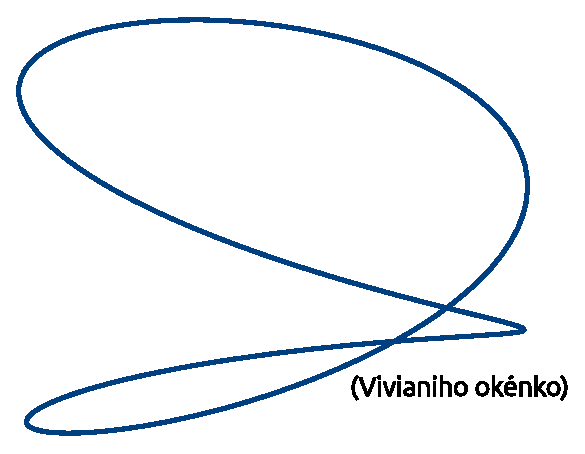
\includegraphics[width = 400pt]{img/viviani-obalka.eps}
	\end{center}
	\vfill
	
\includegraphics[height = 35pt]{img/logo_cvut.eps} \hfill 
\includegraphics[height = 35pt]{img/oppa.eps}
\end{titlepage}
	
\setcounter{tocdepth}{1}
\tableofcontents
	
\chapter{Úvod}
Tato sbírka úloh vznikla jako maturitní práce na Smíchovské střední průmyslové škole ve školním roce 2013/2014
v rámci projektu Evropské unie OPPA ve spolupráci s Fakultou architektury Českého vysokého učení technického v Praze.	\\[10pt]
K matematice mám kladný vztah a proto jsem si vybral téma týkající se právě matematiky, konkrétně parametrický popis rovinných a prostorových křivek. Vzhledem k tomu, že k pochopení matematiky jsou důležité názorné příklady, rozhodl jsem se vytvořit sbírku řešených příkladů. Doplnil jsem též ukázky křivek z praxe. \\
Látka navazuje na středoškolskou matematiku, od čtenáře se předpokládá znalost analytické geometrie a znalost derivování. \\[10pt]
Text byl vytvořen v programu \LaTeX{}, obrázky rovinných křivek v programech \textit{Geogebra} a \textit{Sage Math}
a obrázky prostorových křivek byly vytvořeny v programovacím jazyku \textit{Python} za použití knihovny \textit{Matplotlib}. Další úpravy
obrázků byly provedeny ve vektorovém grafickém editoru \textit{Inkscape}. Všechen software použitý při tvorbě sbírky je volně
dostupný pod svobodnými licencemi. \\[10pt]
\chapter{Kuželosečky}
Kuželosečky nazýváme také kvadratické křivky, neboť mohou být popsáný pomocí kvadratického polynomu dvou proměnných
\textit{x} a \textit{y}. Obecná rovnice kuželosečky je
$$Ax^2+By^2+Cx+Dy+Exy+F=0$$
(alespoň jedno z čísel
\textit{A}, \textit{B}, \textit{E} je nenulové). \\
Takto mohou být popsány regulární kuželosečky (kružnice, elipsa,
parabola, hyperbola) i singulární kuželosečky (jeden bod, jedna přímka, dvě různoběžné přímky, dvě rovnoběžné přímky) a prázdná množina. \\[5pt]
Jsou-li osy regulárních kuželoseček rovnoběžné se souřadnicovými osami soustavy souřadné $(O, x, y)$, v obecné rovnici
se nevyskytuje člen $Exy$, tj. $E=0$. V dalším textu se budeme zabývat výhradně regulárními kuželosečkami s osami rovnoběžnými
se souřadnicovými osami. \\
Připomeňme, jak z obecné rovnice poznáme, o jakou kuželosečku se jedná. \\
Je-li jedno z čísel \textit{A}, \textit{B} nulové, kuželosečka je parabola. \\
Je-li $A \cdot B > 0$, je kuželosečka elipsa, \\
je-li navíc $A=B$, je kuželosečka kružnice. \\
Je-li $A \cdot B < 0$, je kuželosečka hyperbola. \\[10pt]
U elipsy a hyperboly převedeme obecnou rovnici na středový tvar, pak snadno určíme souřadnice středu a velikost poloos.
U paraboly převedeme obecnou rovnici na vrcholový tvar a snadno určíme souřadnice vrcholu a parametr. \newpage
\section{Kružnice}
Pro určování hodnot goniometrických funkcí využíváme jednotkovou kružnici $x^2+y^2=1$.
Souřadnice bodu kružnice jsou $x=\cos{t}$ a $y=\sin{t}$, kde \textit{t} je orientovaný úhel.
\begin{figure}[H]
	\centering
	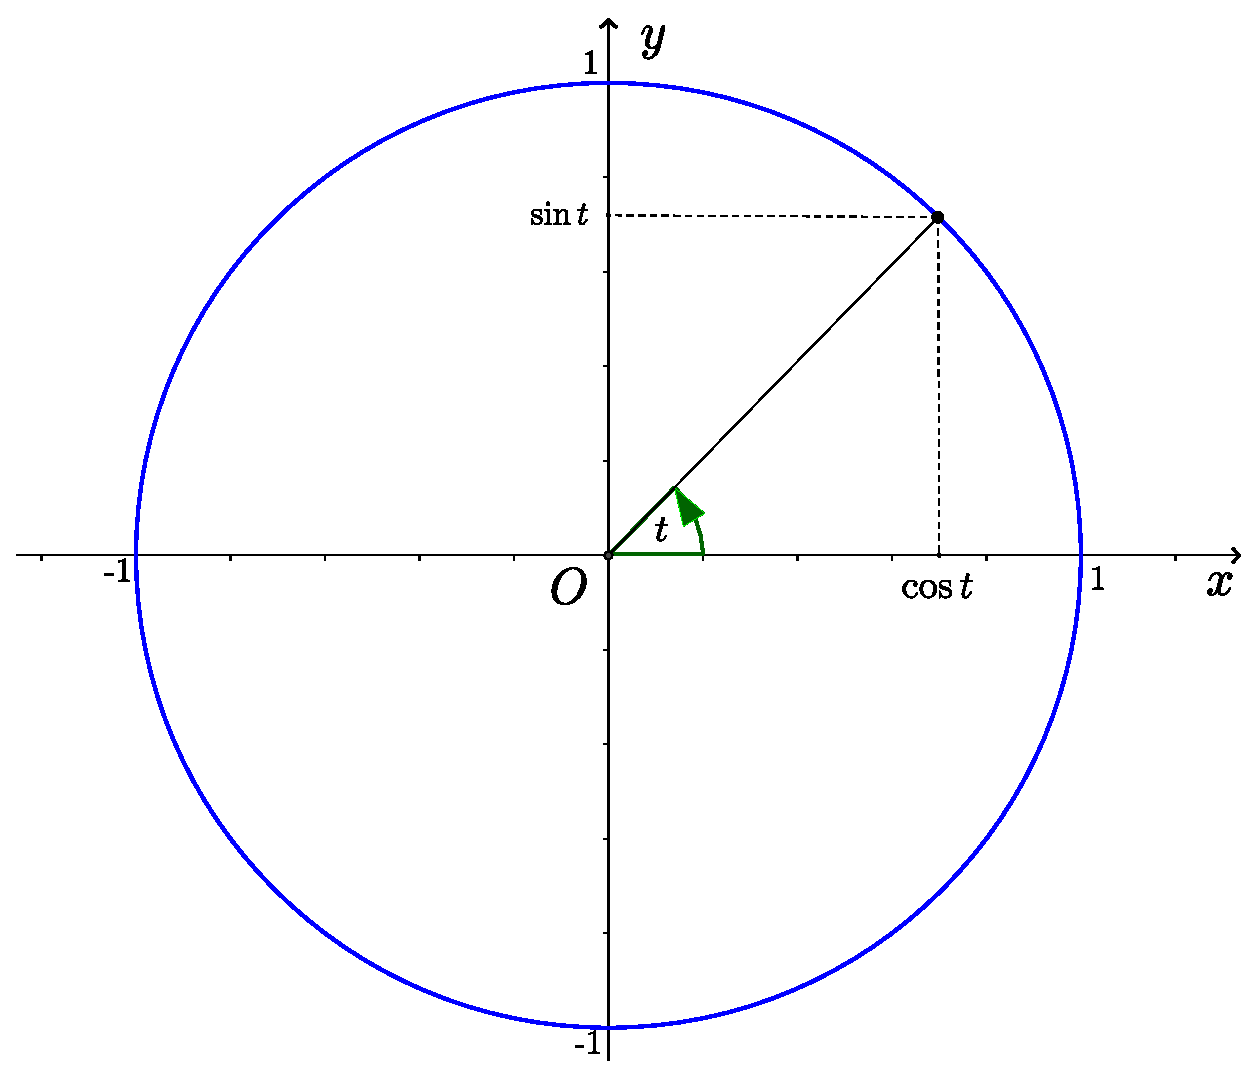
\includegraphics[width=0.5\textwidth]{jednotkovakruznice.eps}
	\caption{Jednotková kružnice}
\end{figure}
\noindent Kružnici můžeme tedy popsat takto
$$k(t)=[\cos{t}, \sin{t}]$$
a to je právě parametrický popis kružnice (také parametrické rovnice kružnice), \textit{t} se nazývá
parametr. Parametr \textit{t} je proměnný a jeho hodnoty můžeme vybírat z různých intervalů: \\
\begin{tabular}{ll}
	$t \in \mathbb{R}$             & kružnice je probíhána neustále                                                                                       \\  
	$t \in \langle 0, 2\pi\rangle$ & výchozí bod je $k(0)=[\cos{0}, \sin{0}] = [1, 0]$                                                                      \\ 
	                               & koncový bod je $k\left(2\pi\right)=[\cos{2\pi}, \sin{2\pi}] = [1, 0]$                                                   \\ 
	                               & jeden oběh kružnice                                                                                                    \\ 
	$t \in \langle 0, 4\pi\rangle$ & výchozí bod je $k(0) = [1, 0]$                                                                                         \\ 
	                               & koncový bod je $k\left(4\pi\right) = [1, 0]$                                                                            \\ 
	                               & dva oběhy kružnice                                                                                                     \\ 
	$t \in \langle 0, \pi\rangle$  & výchozí bod je $k(0) = [1, 0]$                                                                                         \\ 
	                               & koncový bod je $k\left(\pi\right)=[-1, 0]$                                                                              \\ 
	                               & popis půlkružnice (horní půlkružnice)                                                                               \\ 
	$t \in \left\langle -\frac{\pi}{2}, \frac{\pi}{2}\right\rangle$
	                               & výchozí bod je $k\left(-\frac{\pi}{2}\right) = \left[\cos{(-\frac{\pi}{2})}, \sin{(-\frac{\pi}{2})}\right]  = [0, -1]$ \\ 
	                               & koncový bod je $k\left(\frac{\pi}{2}\right) = [0, 1]$                                                                   \\ 
	                               & popis půlkružnice (pravá půlkružnice)                                                                               \\ 
	$t \in \left\langle -\frac{3\pi}{4}, \frac{\pi}{3}\right\rangle$
	                               & výchozí bod je $k\left(-\frac{3\pi}{4}\right)  = \left[-\frac{\sqrt{2}}{2}, -\frac{\sqrt{2}}{2} \right]$               \\ 
	                               & koncový bod je $k\left(\frac{\pi}{3}\right)  = \left[\frac{1}{2}, \frac{\sqrt{3}}{2} \right]$                           \\ 
	                               & popis části kružnice                                                                                                  \\ 
\end{tabular}\\
\begin{figure}
	\centering
	\begin{subfigure}[b]{0.3\textwidth}
		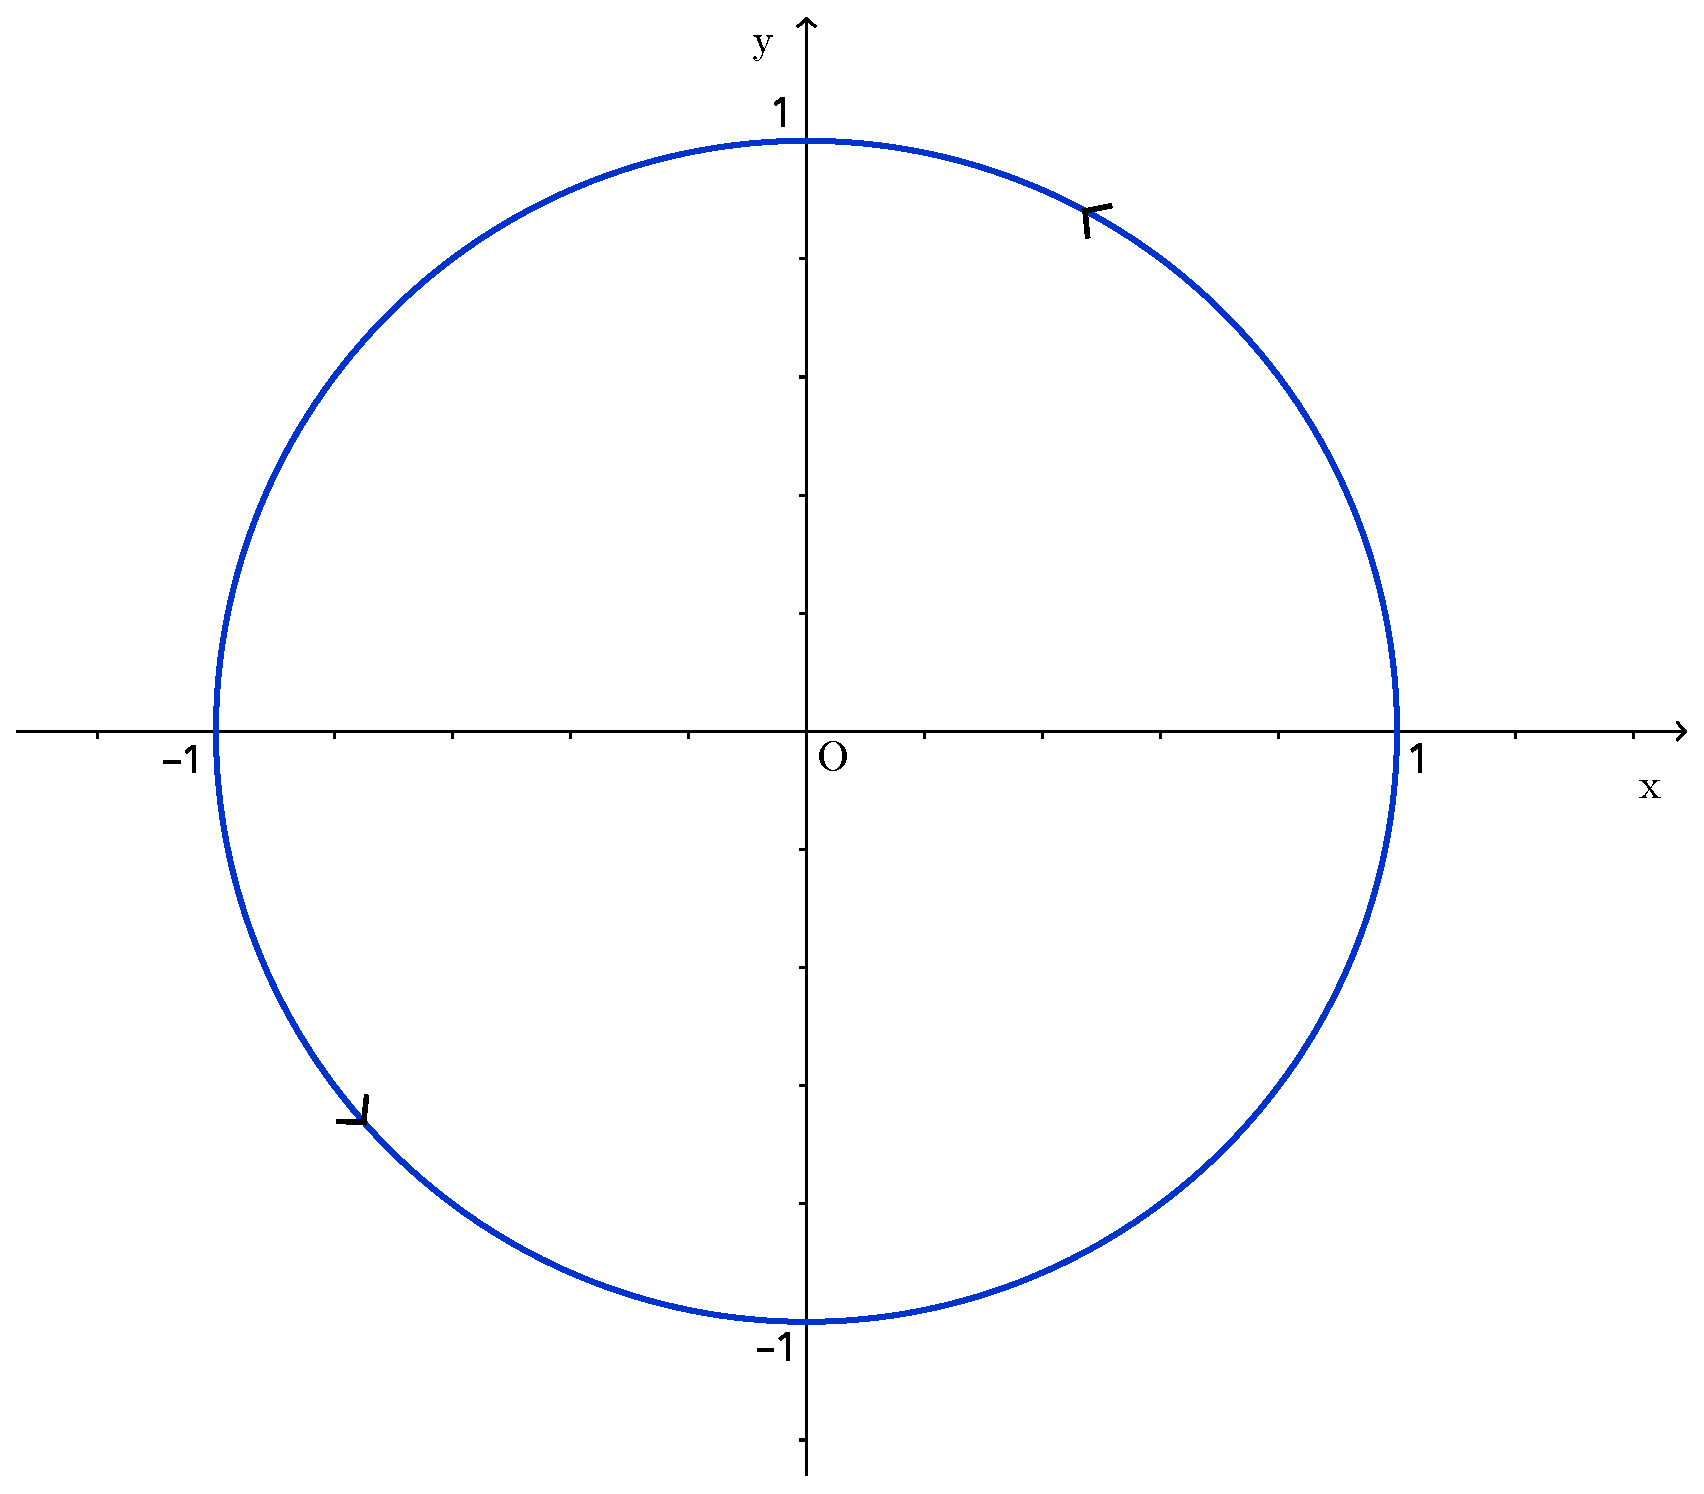
\includegraphics[width=\textwidth]{kruznice-teorie1.eps}
		\caption{$t \in \mathbb{R}$}
	\end{subfigure}%
	\quad
	\begin{subfigure}[b]{0.3\textwidth}
		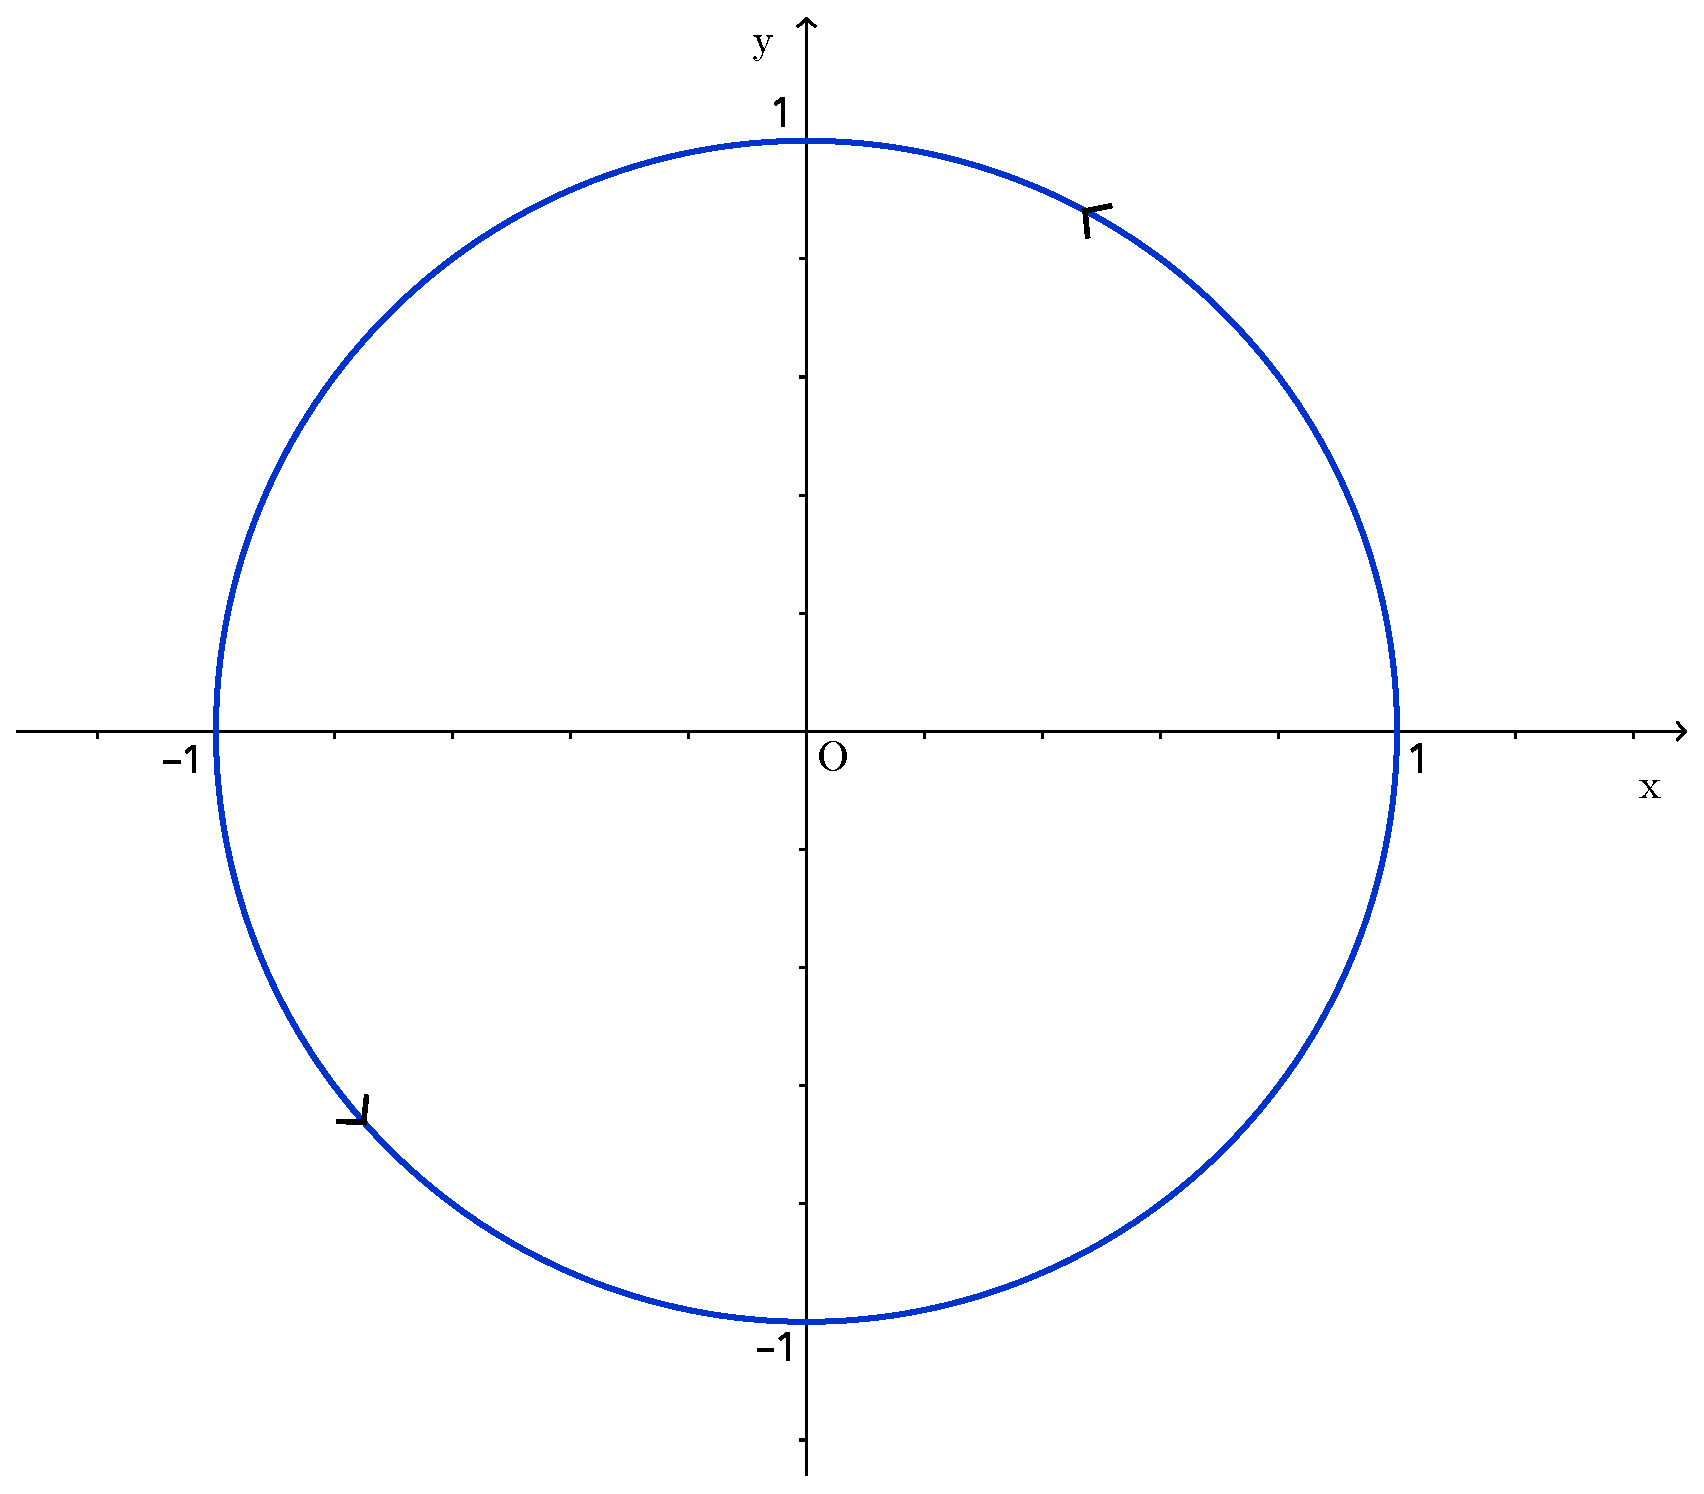
\includegraphics[width=\textwidth]{kruznice-teorie1.eps}
		\caption{$t \in \langle 0, 2\pi\rangle$}
	\end{subfigure}%
	\quad
	\begin{subfigure}[b]{0.3\textwidth}
		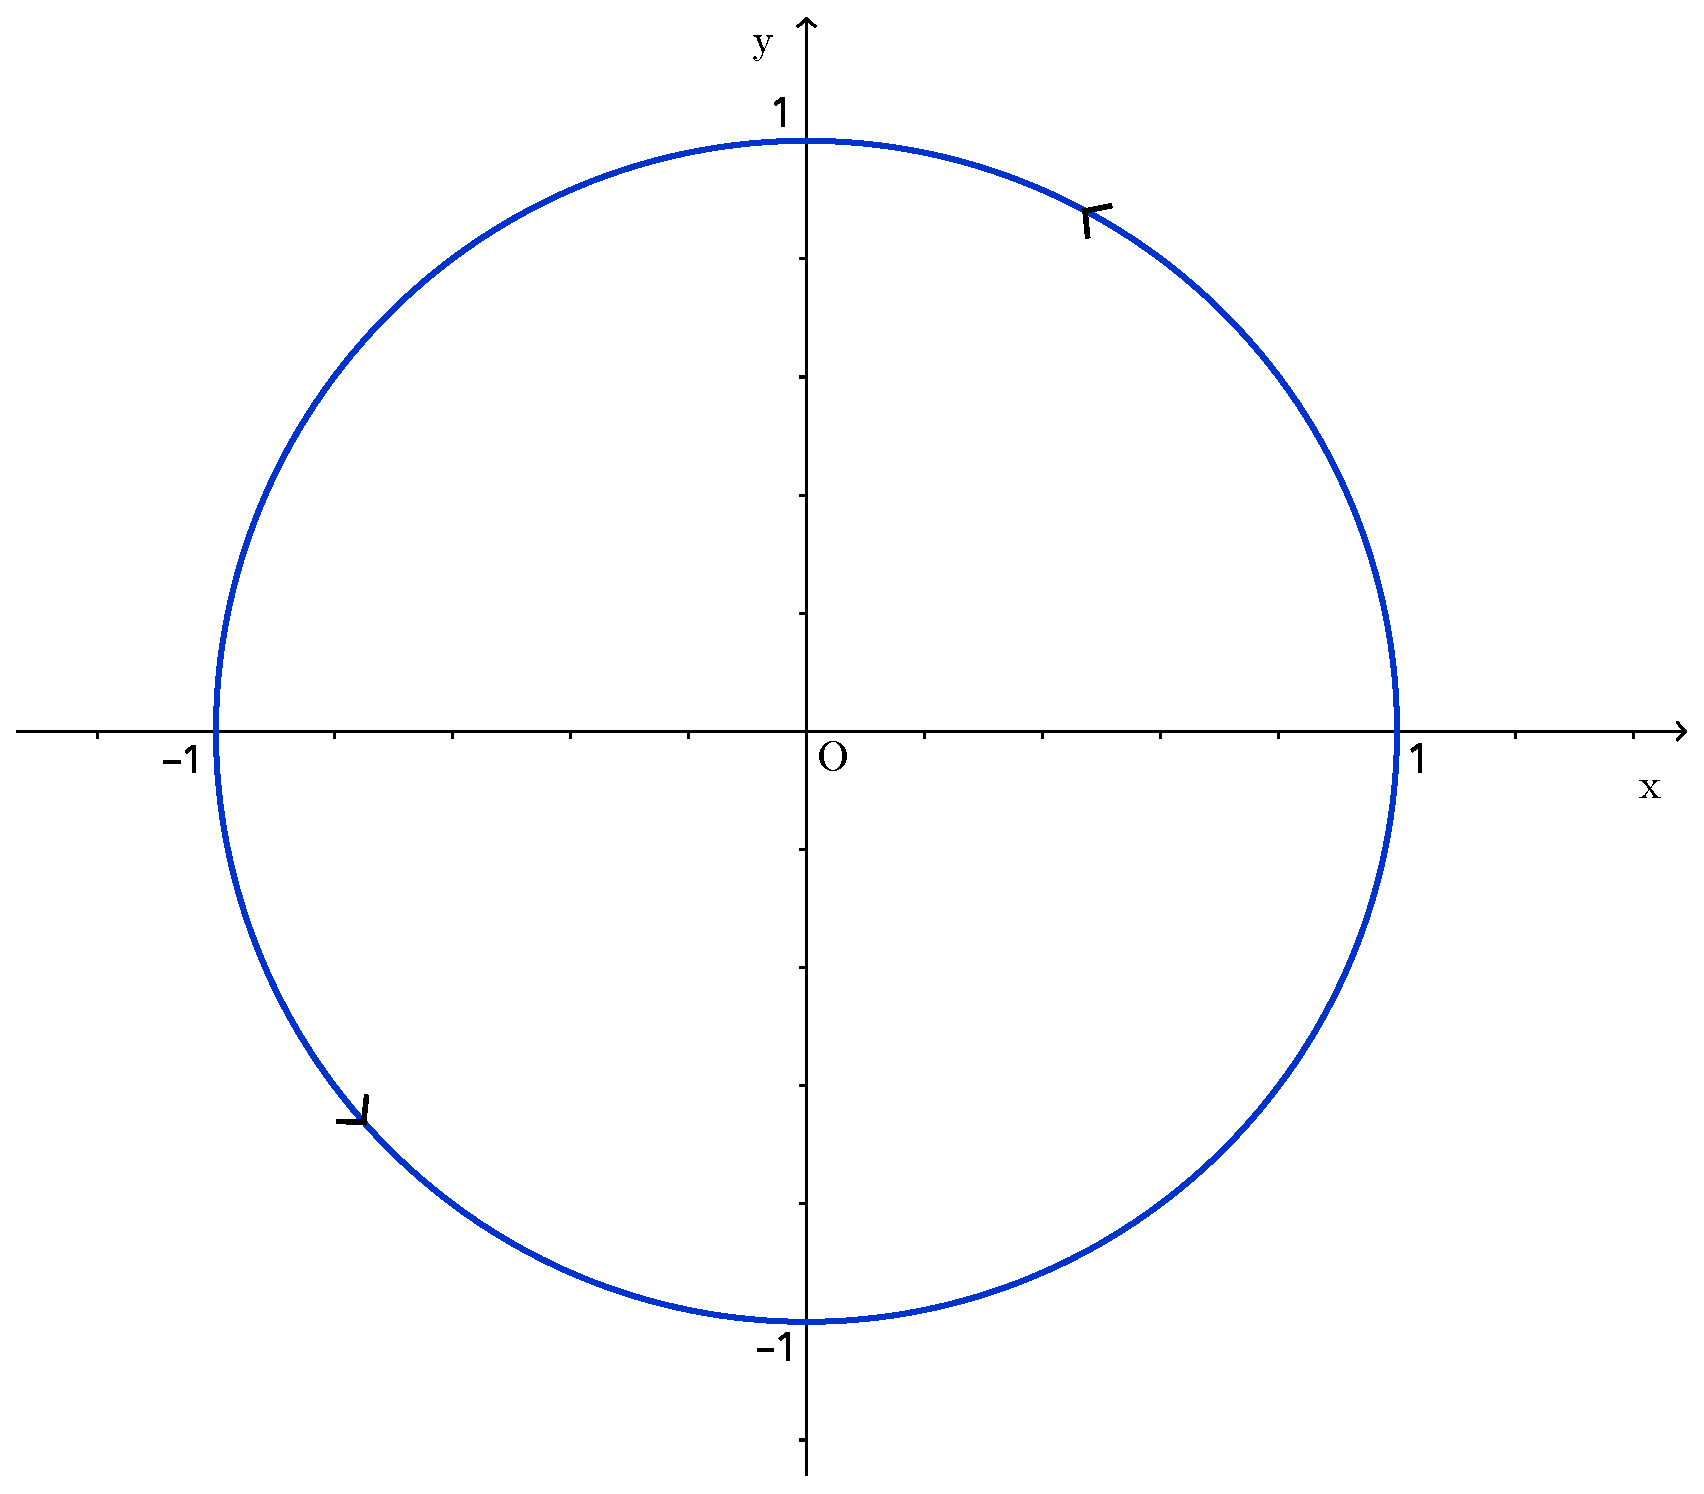
\includegraphics[width=\textwidth]{kruznice-teorie1.eps}
		\caption{$t \in \langle 0, 4\pi\rangle$}
	\end{subfigure}%
	\\
	\begin{subfigure}[b]{0.33\textwidth}
		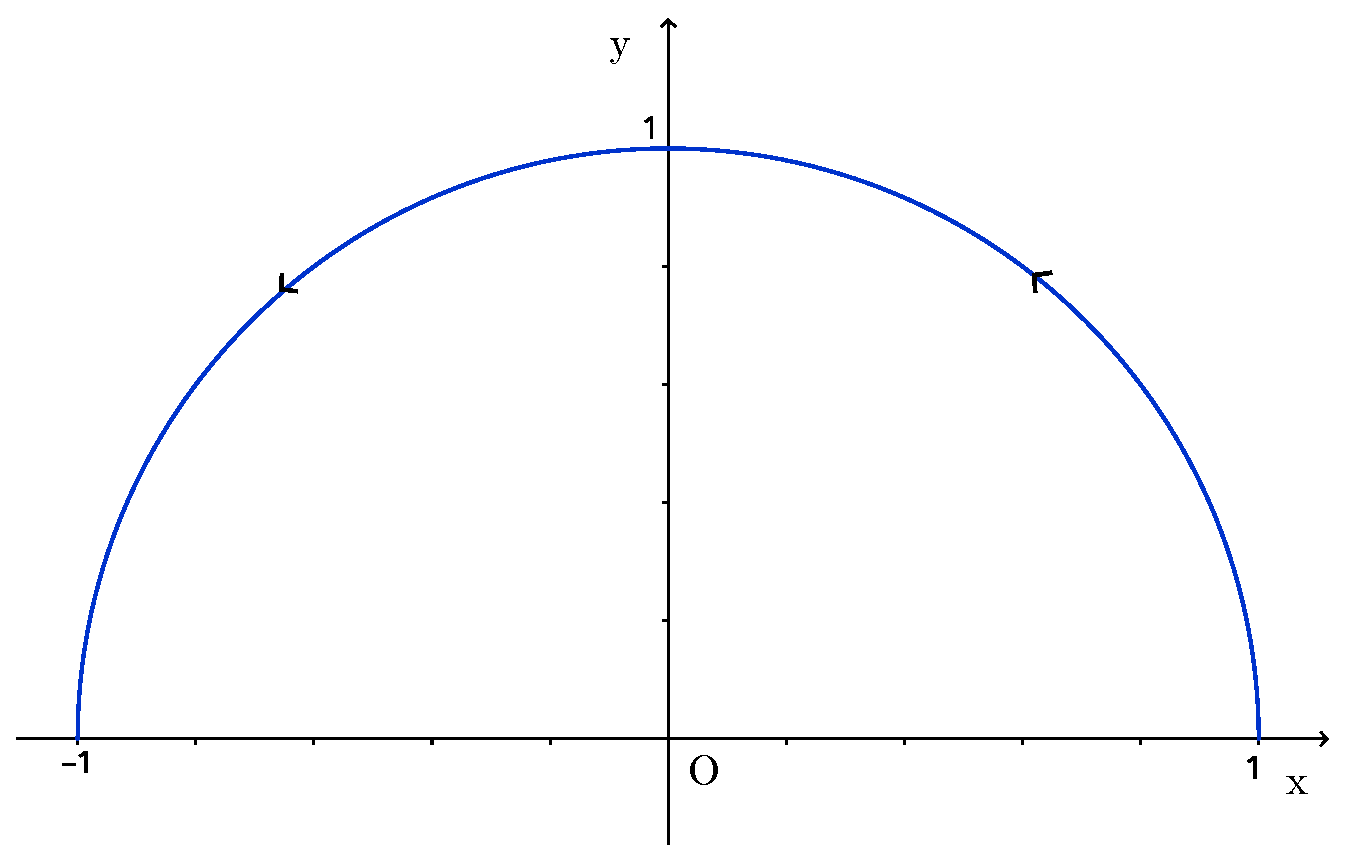
\includegraphics[width=\textwidth]{kruznice-teorie2.eps}
		\caption{$t \in \langle 0, \pi\rangle$}
	\end{subfigure}%
	\begin{subfigure}[b]{0.33\textwidth}
		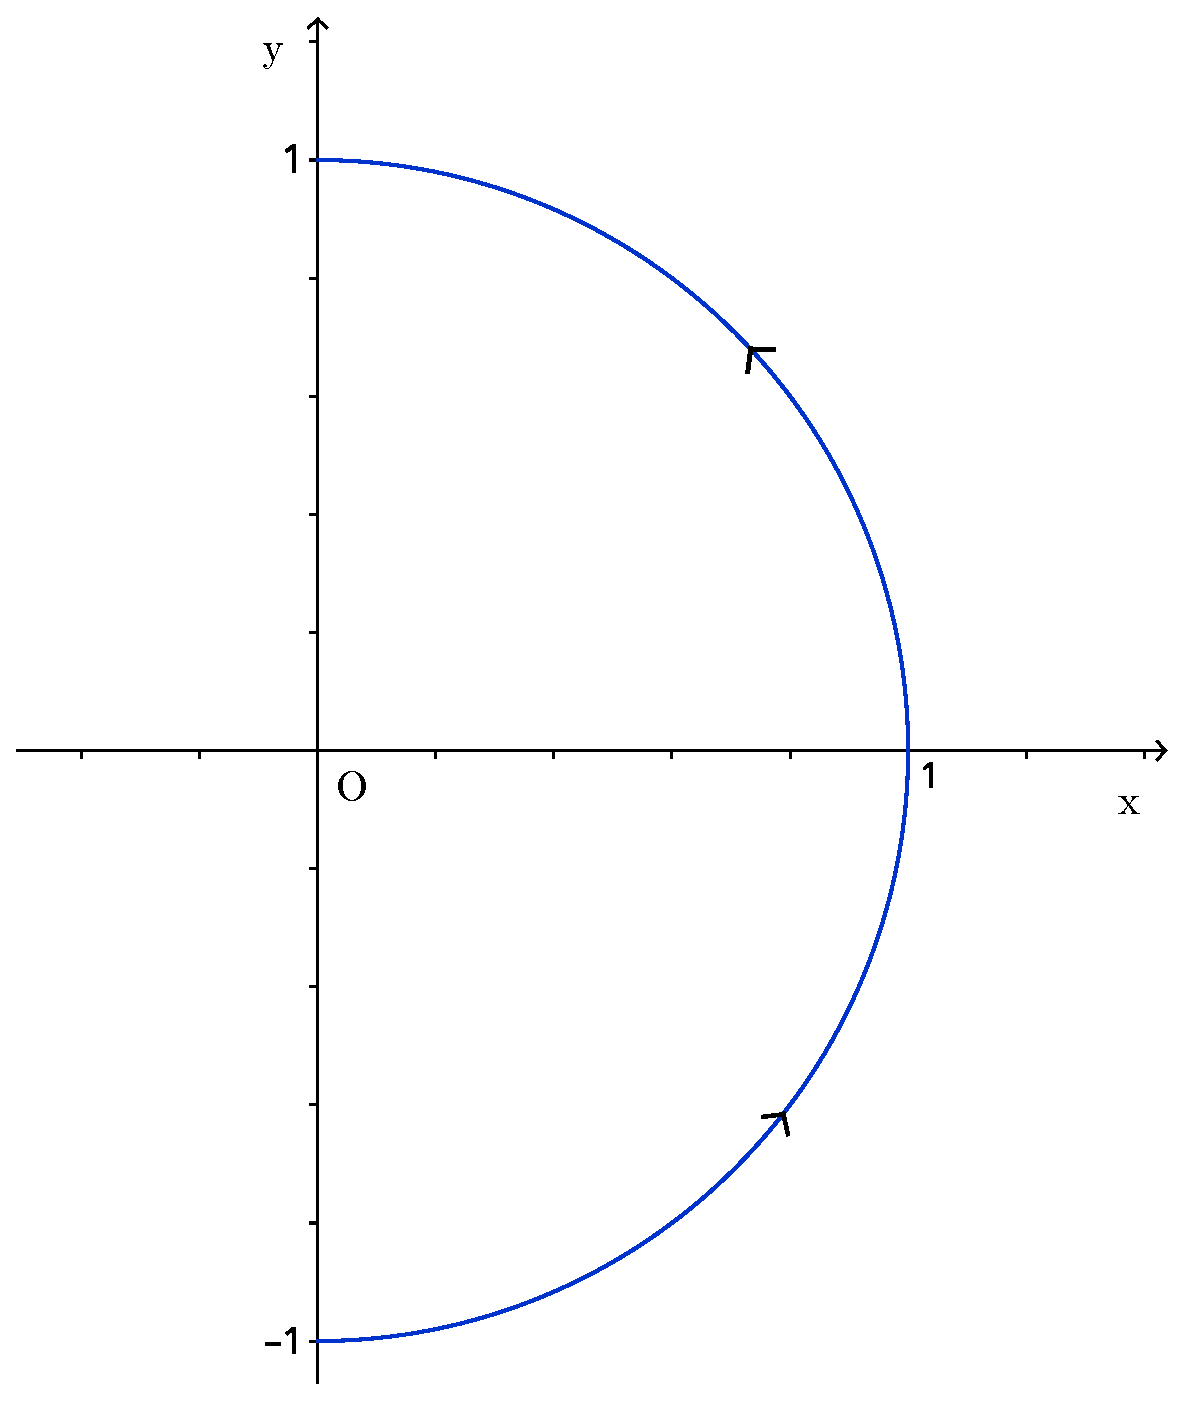
\includegraphics[width=\textwidth]{kruznice-teorie3.eps}
		\caption{$t \in \left\langle -\frac{\pi}{2}, \frac{\pi}{2}\right\rangle$}
	\end{subfigure}%
	\begin{subfigure}[b]{0.33\textwidth}
		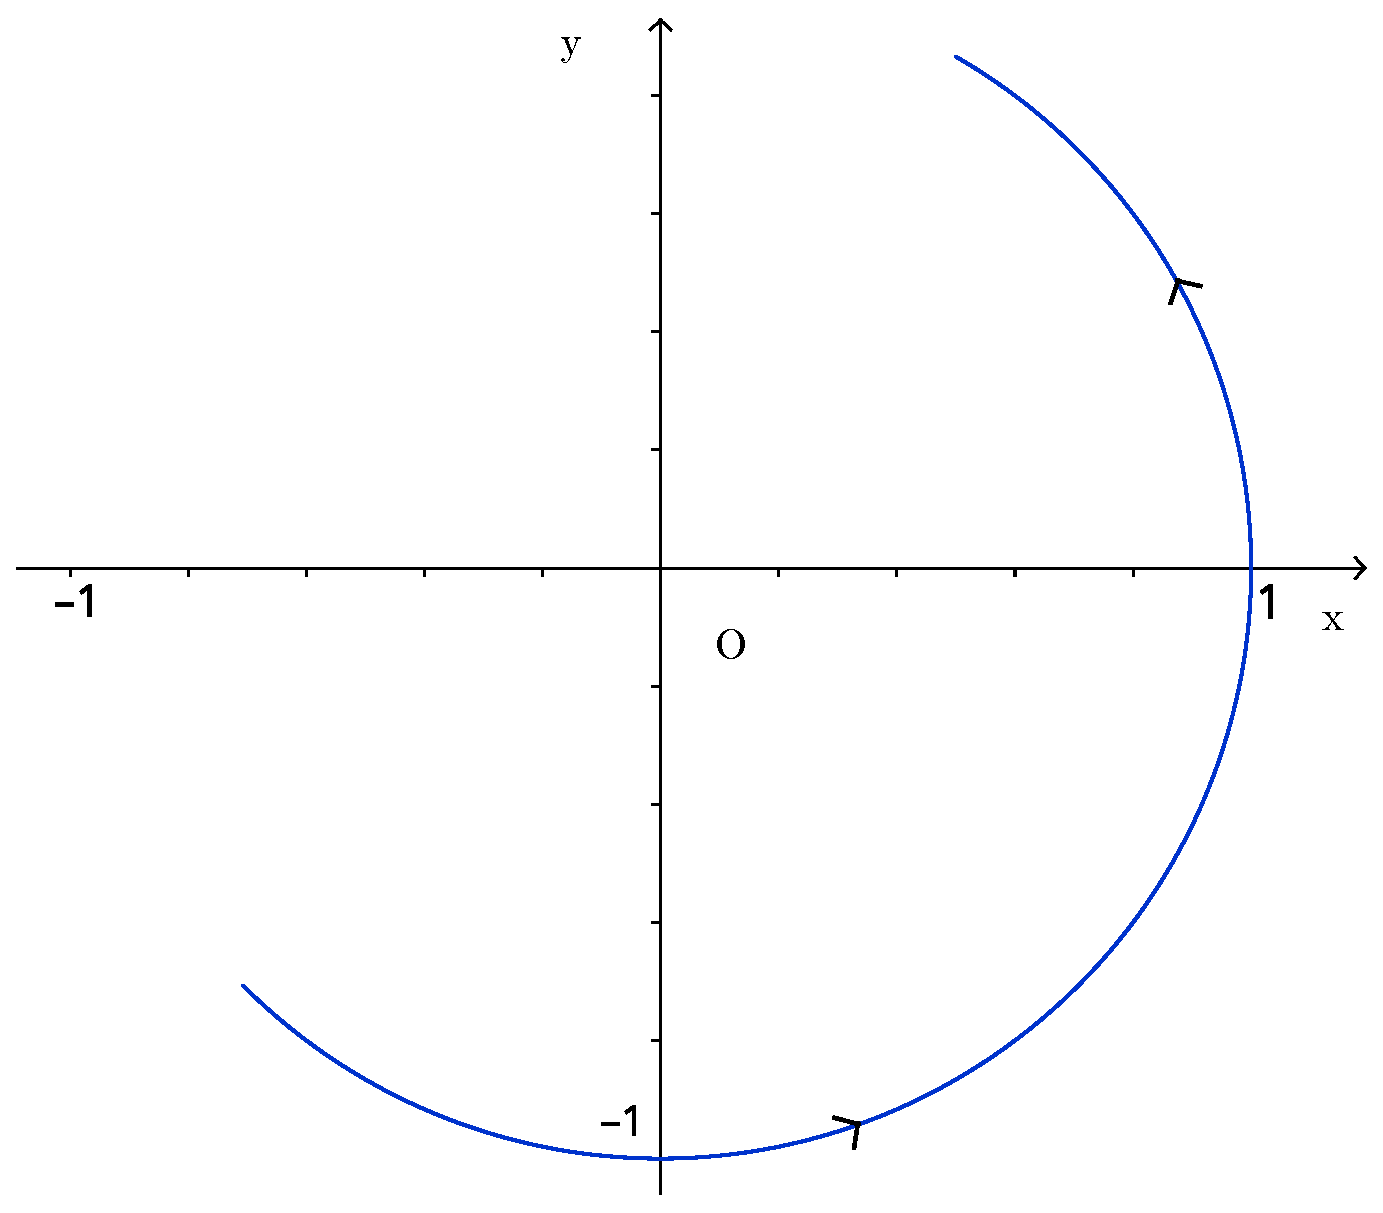
\includegraphics[width=\textwidth]{kruznice-teorie4.eps}
		\caption{$t \in \left\langle -\frac{3\pi}{4}, \frac{\pi}{3}\right\rangle$}
	\end{subfigure}%
	\caption{Kružnice \textit{k} pro různé intervaly parametru \textit{t}}
\end{figure}
\\
\noindent{}Při parametrickém vyjádření $k(t) = [\cos{t}, \sin{t}]$ je kružnice, či její část, probíhána vždy v kladném směru
(tj. proti směru hodinových ručiček). \\
Jak parametrický popis upravit, aby byla kružnice nebo její část probíhána v záporném směru? Zkusíme zaměnit parametr \textit{t} hodnotou $-t$:
$$k(t)=[\cos{(-t)}, \sin{(-t)}] = [\cos{t}, -\sin{t}]$$
(využíváme, že $\cos$ je sudá funkce a $\sin$ je lichá funkce). \\[5pt]
Uvažujme pro parametr \textit{t} interval $ \langle 0, 2\pi\rangle$. \\
Snadno vypočítáme $k(0)=[1,0]$, $k\left(\frac{\pi}{2}\right)=[0,-1]$, 
$k(\pi)=[-1,0]$ a $k(2\pi)=[1,0]$. Výchozí i koncový bod je $[1, 0]$
a kružnice je probíhána v záporném směru (tj. ve směru hodinových ručiček). \\
Můžeme vyzkoušet i další kombinace. Pro jeden oběh kružnice je výhodné použít vždy interval $\langle0, 2\pi \rangle$. \\
\begin{tabular}{ll}
	$k(t)=[-\cos{t}, \sin{t}]$  & výchozí bod je $k(0)=[-1, 0]$                                           \\ 
	                            & pro určení směru použijeme bod $k\left(\frac{\pi}{2}\right) = [0, 1]$ \\ 
	                            & tj. kružnice je probíhána v záporném směru                          \\ 
	$k(t)=[-\cos{t}, -\sin{t}]$ & výchozí bod je $k(0) = [-1, 0]$                                         \\ 
	                            & $k\left(\frac{\pi}{2}\right) = [0, -1]$                                   \\ 
	                            & tj. kružnice je probíhána v kladném směru                            \\ 
\end{tabular}  \\[5pt]
Ještě můžeme zaměnit souřadnice (stále $t \in \langle0, 2\pi\rangle$): \\
\begin{tabular}{llll}
	$k(t)=[\sin{t}, \cos{t}]$   & $k(0)=[0, 1]$  & $k\left(\frac{\pi}{2}\right) = [1,0]$  & záporný směr \\ 
	$k(t)=[\sin{t}, -\cos{t}]$  & $k(0)=[0, -1]$ & $k\left(\frac{\pi}{2}\right) = [1,0]$  & kladný směr   \\ 
	$k(t)=[-\sin{t}, \cos{t}]$  & $k(0)=[0, 1]$  & $k\left(\frac{\pi}{2}\right) = [-1,0]$ & kladný směr   \\ 
	$k(t)=[-\sin{t}, -\cos{t}]$ & $k(0)=[0, -1]$ & $k\left(\frac{\pi}{2}\right) = [-1,0]$ & záporný směr \\ 
\end{tabular}  \\[5pt]
Pro kružnici, která má střed $[0, 0]$ a její poloměr \textit{r} není roven 1, lze využít podobné popisy
$k(t) = [r\cdot\cos{t}, r\cdot\sin{t}]$, $k(t) = [r\cdot\cos{t}, -r\cdot\sin{t}]$ atd. \\[10pt]
	Ve všech předchozích popisech jednotkové kružnice, kde $t \in \langle0, 2\pi\rangle$, je výchozí bod
	na jedné ze souřadnicových os \textit{x} a \textit{y}. Jak popsat kružnici, aby výchozí bod mohl být
	vybrán obecněji? Jistě bychom mohli změnit interval pro parametr \textit{t}, $t \in \langle\alpha, \beta\rangle$,
	ale určení úhlu $\alpha$ nemusí být vždy jednoduché. Chceme vždy použít pro jeden oběh interval $\langle0, 2\pi\rangle$.
	Vyberme bod $\left[\frac{1}{2}, \frac{\sqrt{3}}{2}\right]$ na jednotkové kružnici. Chceme, aby tento bod byl výchozí
	a kružnice byla probíhána v kladném směru. \\
	Požadujeme $k(0)=\left[\frac{1}{2}, \frac{\sqrt{3}}{2}\right]$ a
	$k\left(\frac{\pi}{2}\right)=\left[-\frac{\sqrt{3}}{2}, \frac{1}{2}\right]$.
	\begin{figure}[H]
		\centering
		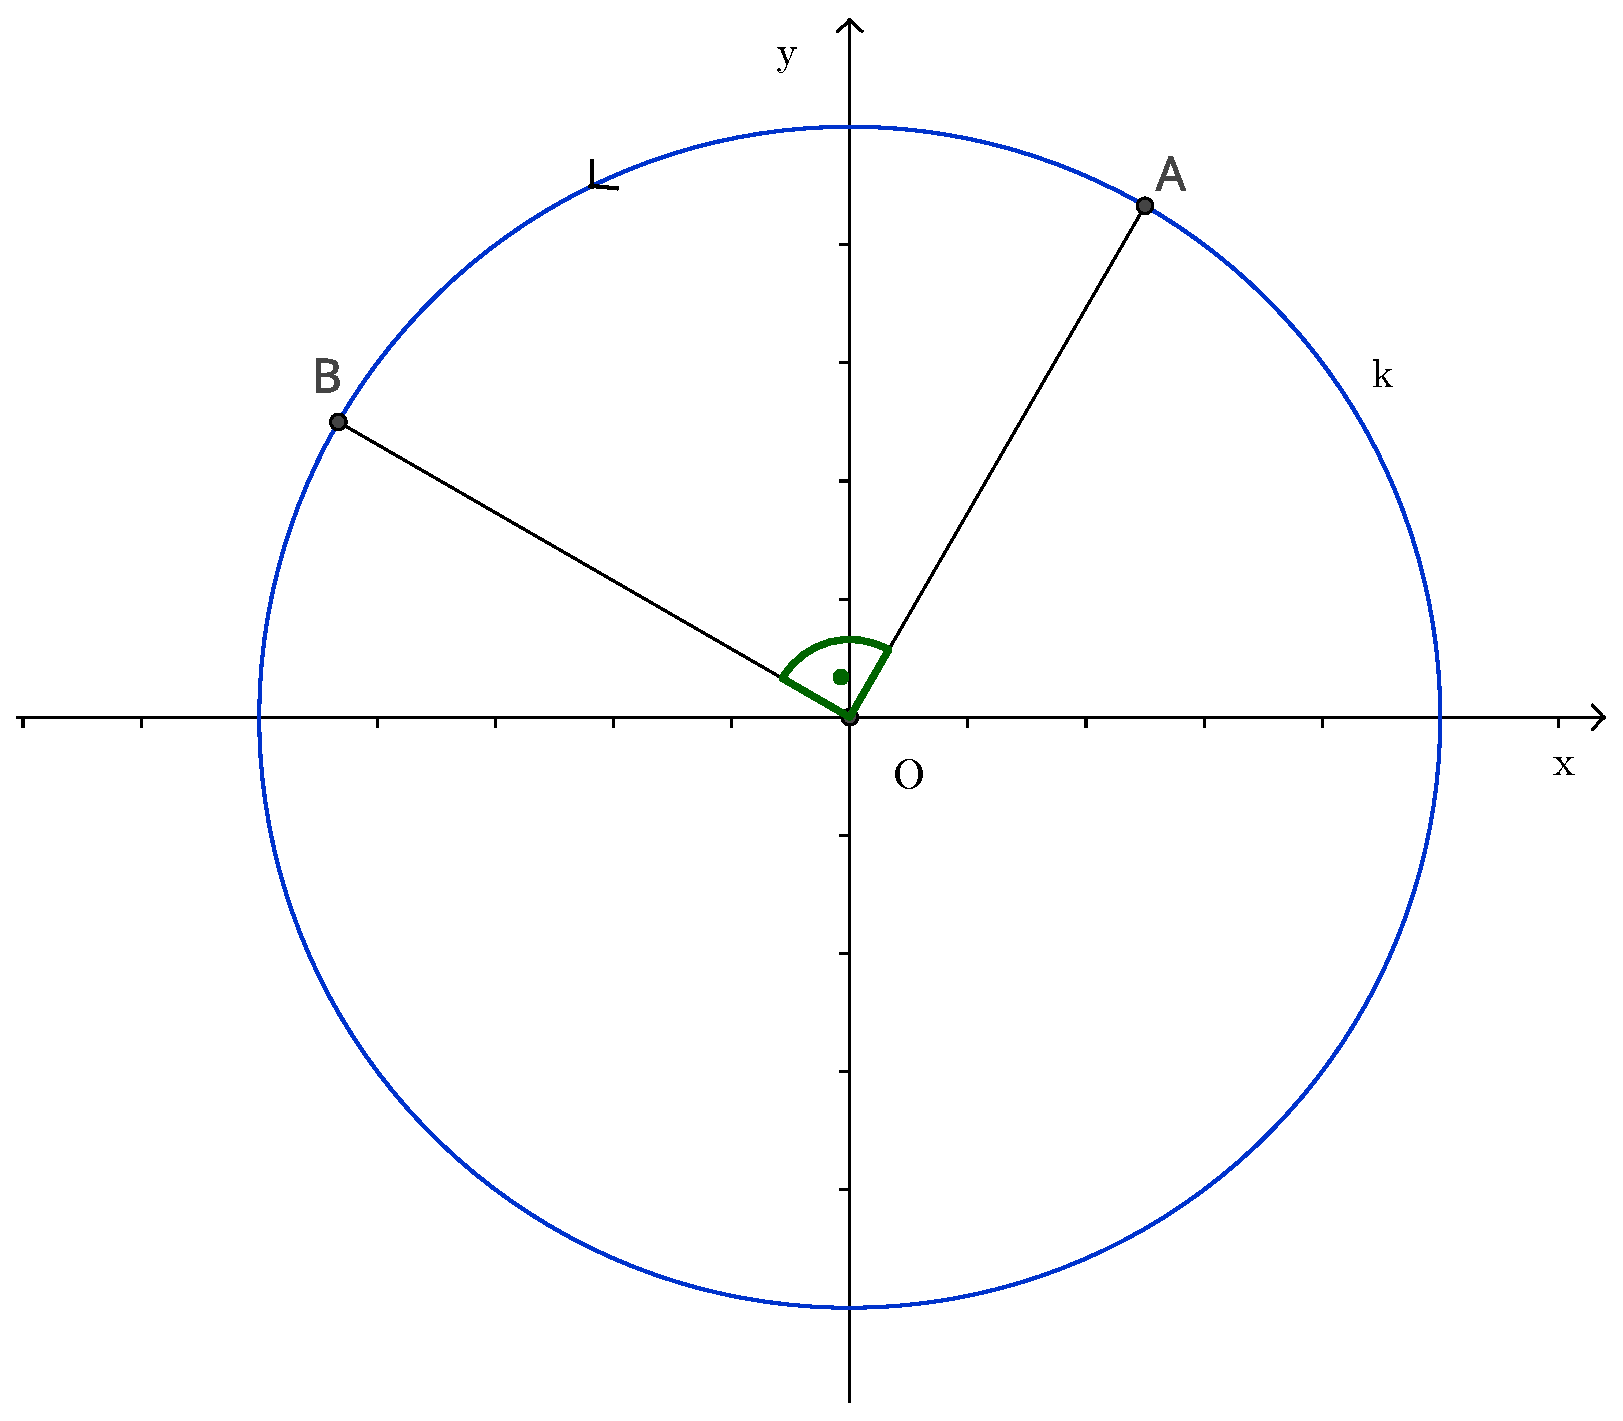
\includegraphics[width=0.45\textwidth]{kruznice-teorie5.eps}
		\caption{Kružnice probíhána z obecného bodu}					
	\end{figure}
	V první i druhé souřadnici parametrického popisu se musí objevit funkce $\cos$ i $\sin$:
	$$ k(t) = \left[\frac{1}{2}\cos{t}-\frac{\sqrt{3}}{2}\sin{t}, \frac{\sqrt{3}}{2}\cos{t}+\frac{1}{2}\sin{t}\right], t \in \langle0, 2\pi\rangle. $$
	Pro oběh kružnice v záporném směru stačí změnit znaménka u funkce $\sin$, jak jsme mohli vypozorovat v předchozím popisu. \\
	Pro kružnici o středu $S=[0, 0]$ a pro výchozí bod $P=[p, q]$ můžeme psát
	$$k(t) = [p\cos{t}-q\sin{t}, q\cos{t} + p\sin{t}], t \in \langle0, 2\pi\rangle \text{, kladný směr},$$
	$$k(t) = [p\cos{t}+q\sin{t}, q\cos{t} - p\sin{t}], t \in \langle0, 2\pi\rangle \text{, záporný směr}.$$
	Lze také použít zápis s využitím vektorů
	$$k(t) = [0, 0] + (p, q)\cos{t}+(-q, p)\sin{t}$$ nebo
	$$k(t) = [0, 0] + (p, q)\cos{t}+(q, -p)\sin{t},$$
	$[0, 0]$ je střed \textit{S}, vektor $(p, q) = P - S$, vektor $(-q, p)$ nebo $(q, -p)$ je kolmý k vektoru $P-S$. \\	
	\noindent Nyní již snadno získáme parametrický popis libovolné kružnice o středu $S=[m, n]$, jejíž výchozí bod je
	bod $P=[p, q]$:
	\begin{figure}[H]
		\centering
		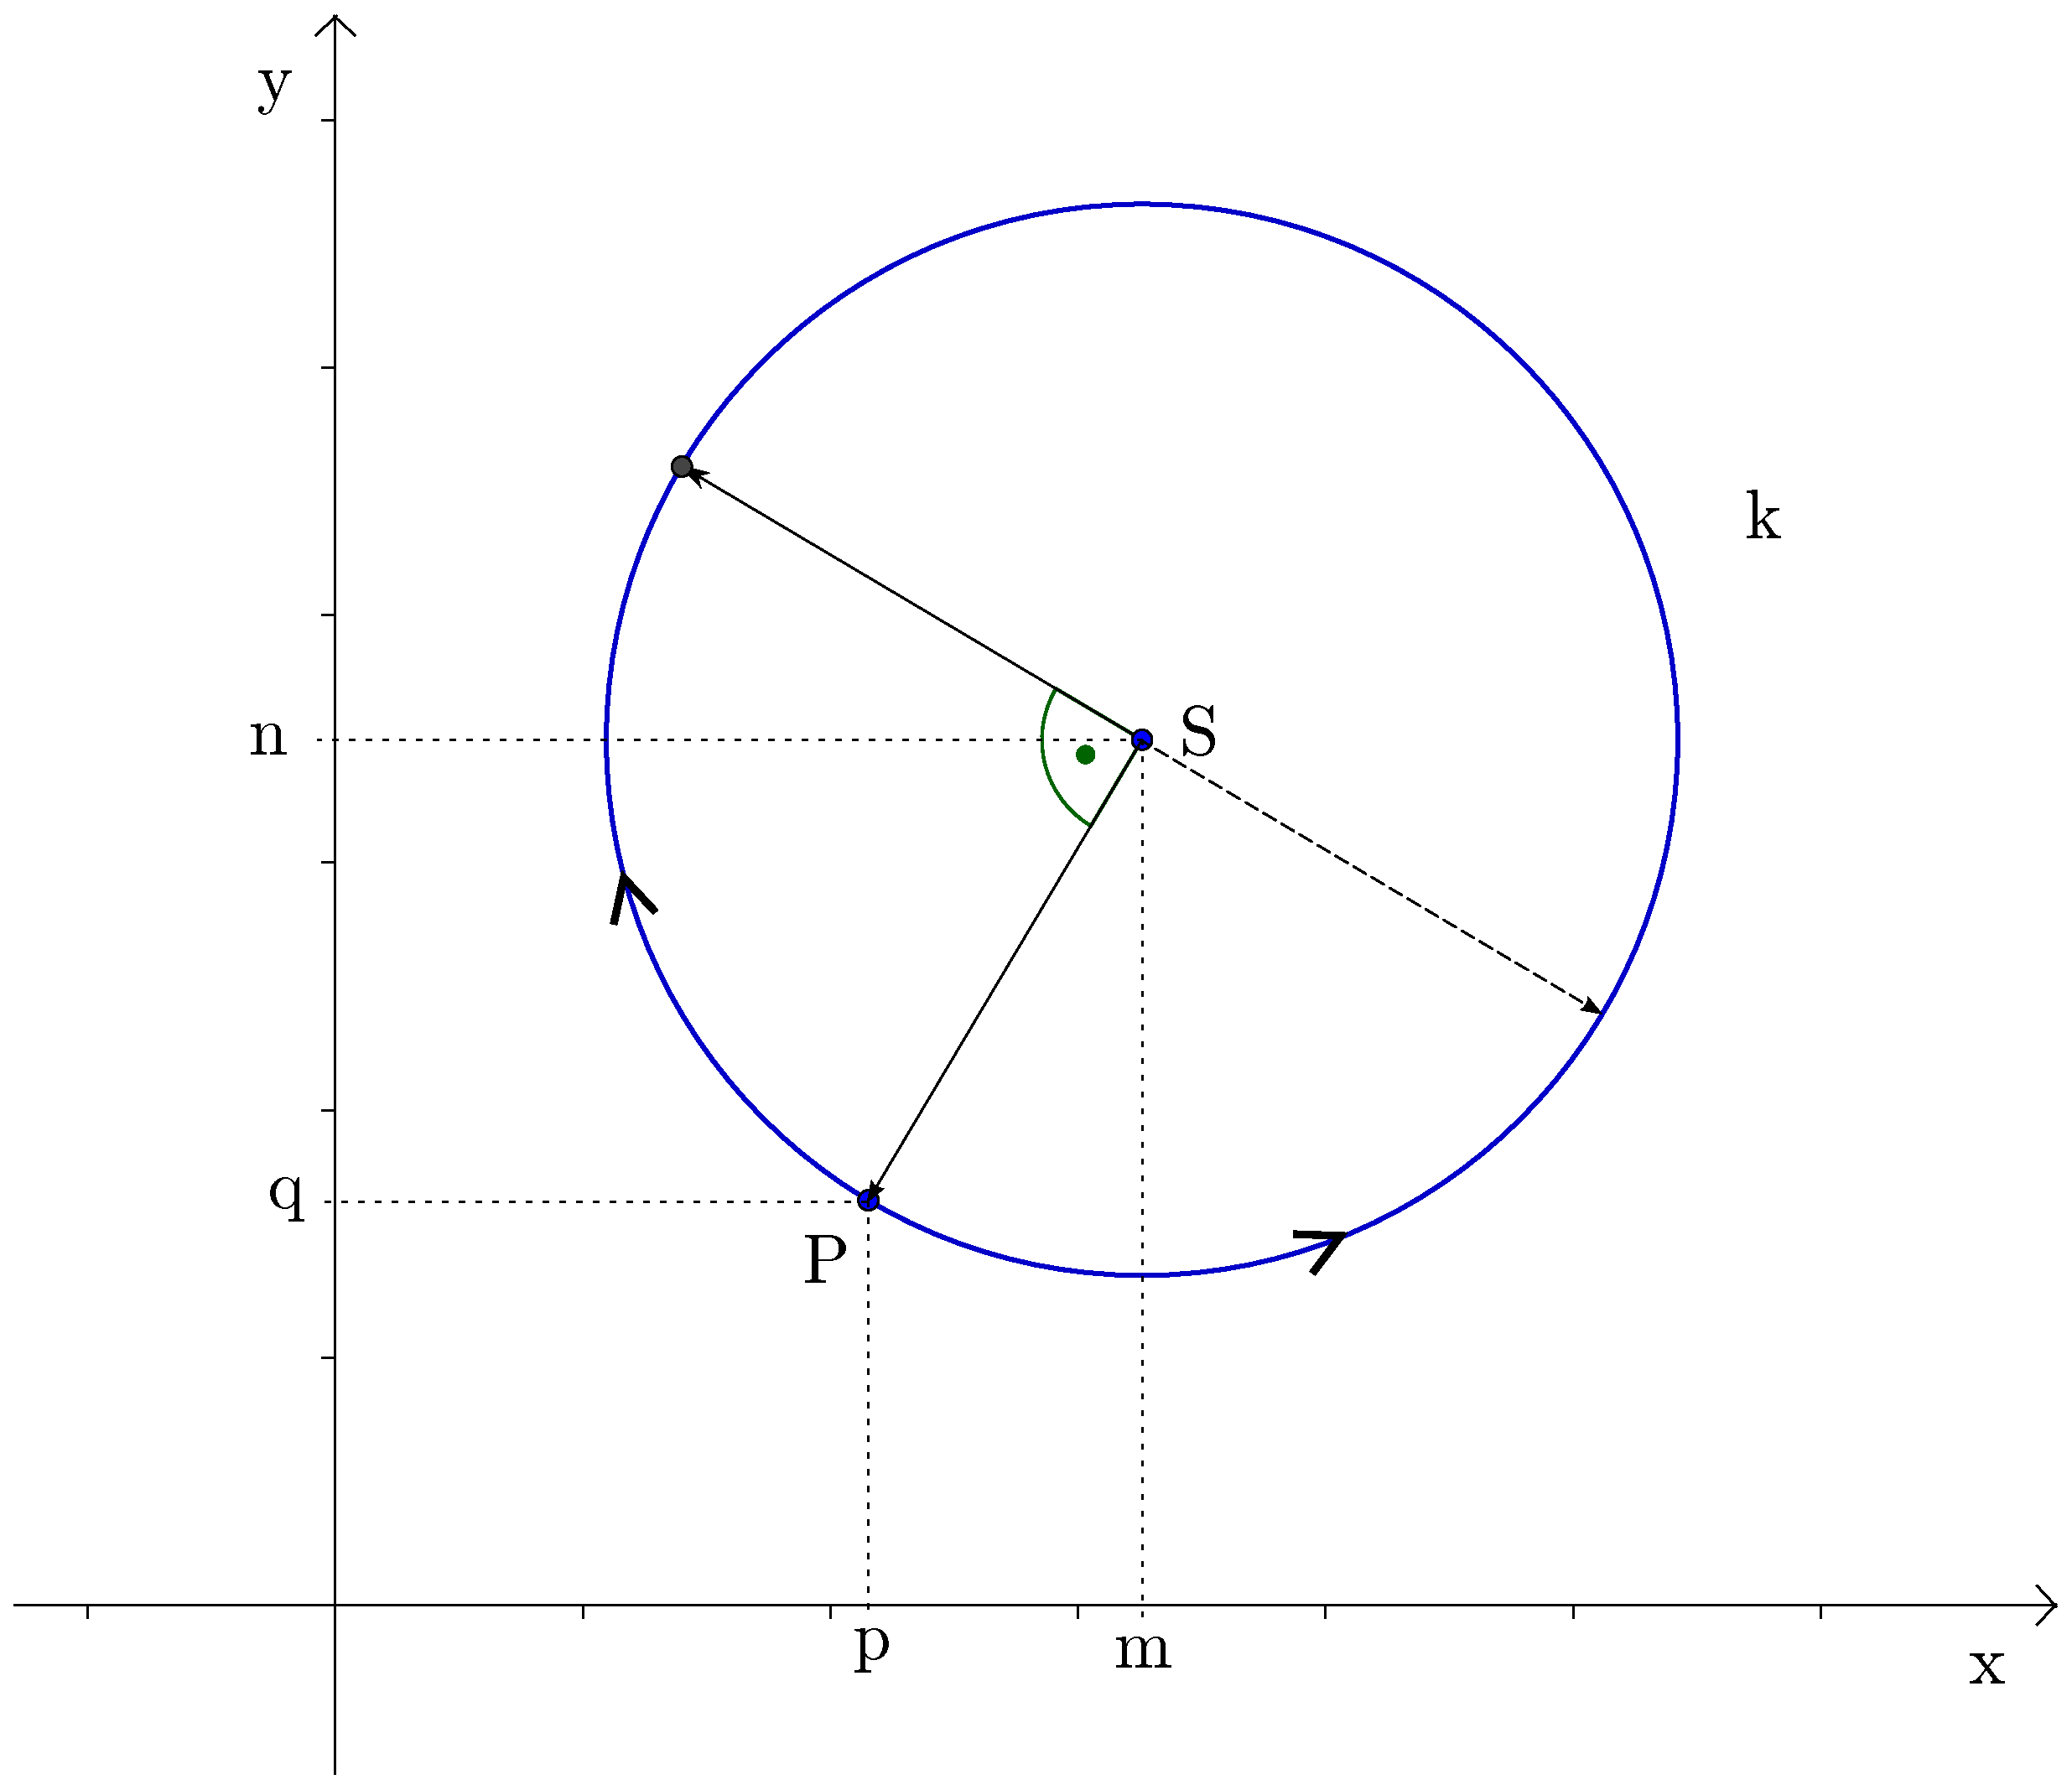
\includegraphics[width=0.5\textwidth]{kruznice-teorie7.eps}
		\caption{Libovolná kružnice probíhána z obecného bodu}					
	\end{figure}	
	$$P-S = (p-m, q-n)$$
	a vektor kolmý je
	$$(-(q-n), p-m), \text{pro kladný směr}$$
	nebo
	$$(q-n, -(p-m)), \text{pro záporný směr}.$$
	Tedy
	$$k(t)=[m, n] + (p-m, q-n)\cos{t} + (-(q-n), p-m)\sin{t}, $$
	tj.:
	$$k(t)=[m + (p-m)\cos{t} - (q-n)\sin{t}, n + (q-n)\cos{t}+(p-m)\sin{t}], t \in \langle0, 2\pi\rangle.$$
	kružnice probíhána (1 oběh) od bodu \textit{P} v kladném směru. \\
	Pro změnu směru stačí změnit znaménko u funkce $\sin$. \\[5pt]
	Tento popis nevyžaduje znalost poloměru kružnice, poloměr si lze ovšem vždy spočítat, je to vzdálenost
	bodů \textit{P}, \textit{S}:
	$$r=\sqrt{(p-m)^2+(q-n)^2}.$$
	Je vidět, že parametrický popis má oproti obecné rovnici navíc důležitou informaci. Parametr \textit{t} si
	můžeme představit jako čas a z parametrického popisu lze vyčíst, jak je křivka probíhána v čase.
	\clearpage
	\subsection*{Příklad}
	Napište parametrické vyjádření kružnice zadané obecnou rovnicí
	$$x^2+y^2-6x-8y=0.$$
	Ověřte, zda kružnice prochází počátkem soustavy souřadné. Pokud ano, napište parametrické
	vyjádření kružnice (jeden oběh), výchozí bod nechť je počátek $[0, 0]$ a kružnice je probíhána
	v záporném směru. \\[10pt]
	\textbf{Řešení:}
	\begin{enumerate}
		\item Obecnou rovnici upravíme na středový tvar
		      $$(x-3)^2+(y-4)^2=25, \text{popř. } \frac{(x-3)^2}{25} + \frac{(y-4)^2}{25}=1.$$
		      Bod $S=[3, 4]$ je střed, poloměr $r=5$. Pokud nám nezáleží, jakým způsobem je kružnice
		      probíhána, můžeme využít vzorec
		      $$\cos^2{t}+\sin^2{t}=1.$$
		      Dáme do rovnosti
		      $$\frac{x-3}{5} = \cos{t}$$
		      a
		      $$\frac{y-4}{5}=\sin{t}$$
		      (nebo $\frac{x-3}{5} = \sin{t}$ a $\frac{y-4}{5}=\cos{t}$). \\
		      Vyjádříme \textit{x} a \textit{y}:
		      $$x=3+5\cos{t},$$
		      $$y=4+5\sin{t}.$$
		      Parametrický popis kružnice je
		      $$k(t) = [3+5\cos{t}, 4+5\sin{t}], t \in \langle0,2\pi\rangle. $$
		      Dosazením $t=0$ a $t=\frac{\pi}{2}$
		      $$k(0) = [8, 4], k\left(\frac{\pi}{2}\right) = [3, 9]$$
		      zjistíme, že výchozí bod je $[8, 4]$ a kružnice je probíhána v kladném směru.
		\item Bod $[0, 0]$ je bodem kružnice (dosadíme do zadané rovnice $x=0$ a $y=0$). \\
		      Nyní můžeme použít vzorec
		      $$k(t)=[m + (p-m)\cos{t} + (q-n)\sin{t}, n + (q-n)\cos{t}-(p-m)\sin{t}], t \in \langle0, 2\pi\rangle$$
		      kde $[m, n] = [3, 4], [p, q] = [0, 0]$. \\[5pt]
		      	Nebo můžeme vyjádřit vektor $O-S=[0, 0] - [3, 4] = (-3, -4)$ a vektor kolmý $(-4, 3)$: \\
		      	$$k(t) = [3, 4] + (-3, -4)\cos{t}+(-4, 3)\sin{t}, t \in \langle0, 2\pi\rangle.$$
		      	$$k(t) = [3-3\cos{t}-4\sin{t}, 4-4\cos{t}+3\sin{t}], t \in \langle0, 2\pi\rangle.$$
		      \end{enumerate}
		      \begin{figure}[H]
		      	\centering
		      	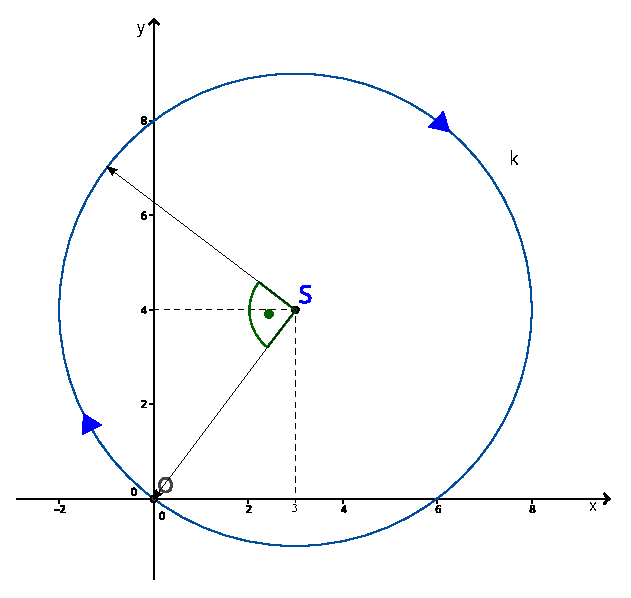
\includegraphics[height = 275pt]{kruznice4.eps}
		      	\caption{Kružnice probíhána v záporném směru  pro $t \in \langle0, 2\pi\rangle$}
		      						
		      \end{figure}
		      \clearpage
		      \section{Parabola}
		      Uvažujme známou parabolu $y=x^2$.\\
		      Tato rovnice je ve vrcholovém tvaru a vrchol paraboly je bod $[0,0]$, osa paraboly je osa \textit{y}. \\
		      Parametr \textit{p} je $p=\frac{1}{2}$ ($x^2=2py$, $2p=1$).
		      Parametr je vzdálenost ohniska \textit{F} od řídící přímky \textit{d}. Ohnisko má souřadnice $F=\left[0, \frac{1}{4}\right]$, řídící přímka má obecnou rovnici $d: y=-\frac{1}{4}$.
		      \begin{figure}[H]
		      	\centering
		      	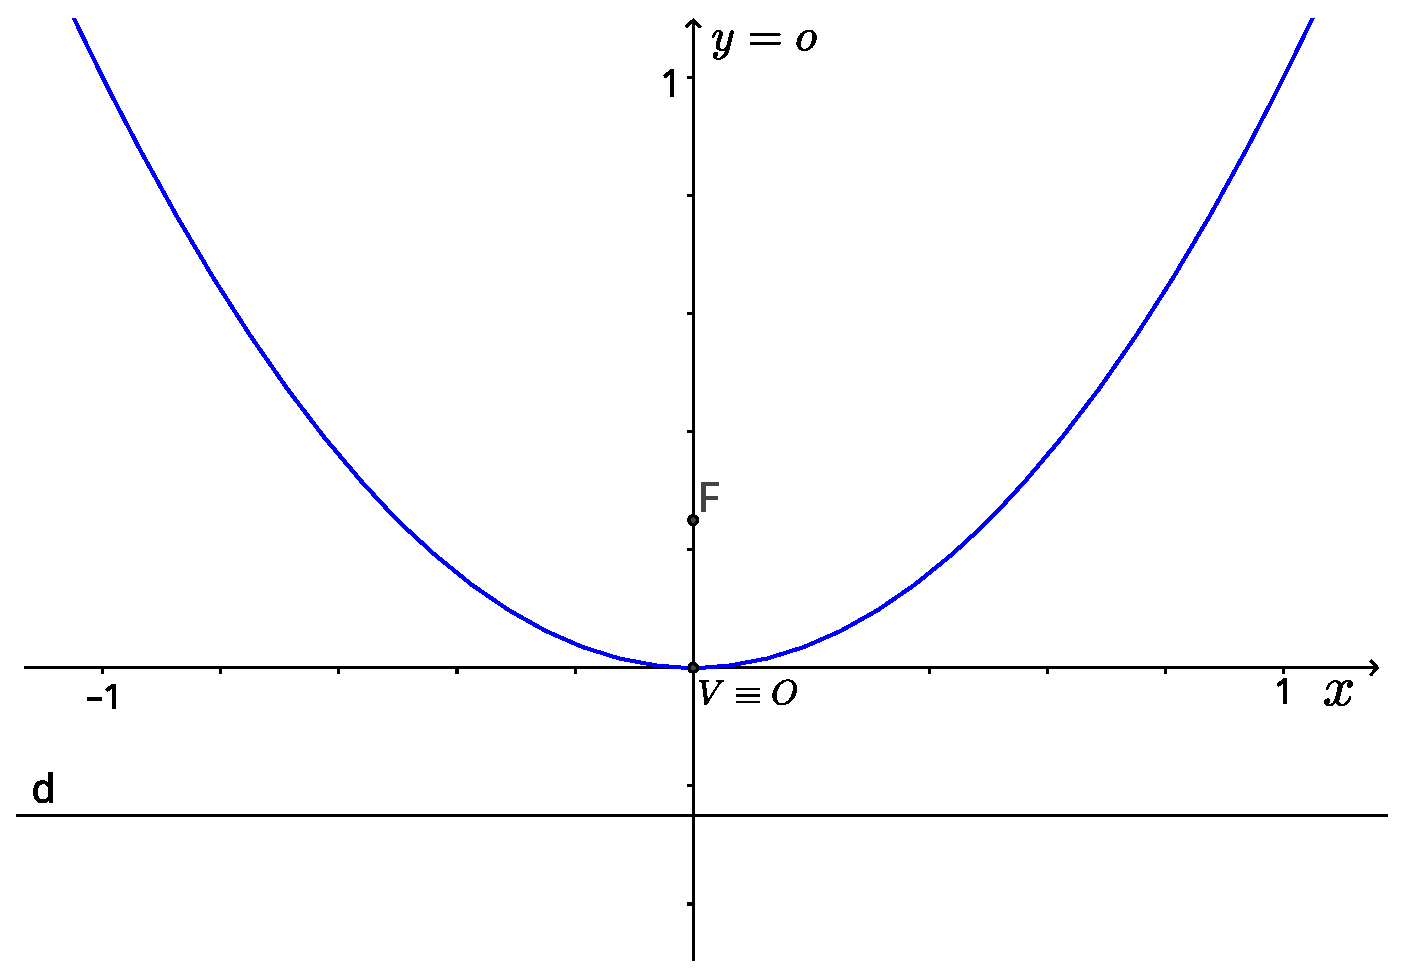
\includegraphics[width=0.5\textwidth]{parabola-teorie1.eps}
		      	\caption{Parabola $y=x^2$}
		      \end{figure}
		      \noindent Souřadnice libovolného bodu jsou $[x, x^2]$. \\
		      Parametrický popis této paraboly je např.:
		      $$k(t) = [t, t^2].$$
		      Aby byla popsána celá parabola, je potřeba pro parametr \textit{t} brát interval $(-\infty, \infty)$, $k(0)=[0,0]$. \\
		      Při kreslení paraboly s využitím grafického programu musíme interval omezit z obou stran, např. $t \in \langle-10, 10\rangle$.
		      \clearpage
		      Parametrických popisů zadané paraboly je stejně jako u kružnice nekonečné mnoho a liší se tím, jak je parabola probíhána.
		      $$k(t)=[t, t^2], t \in \langle-3,3\rangle$$
		      \begin{figure}[H]
		      	\centering
		      	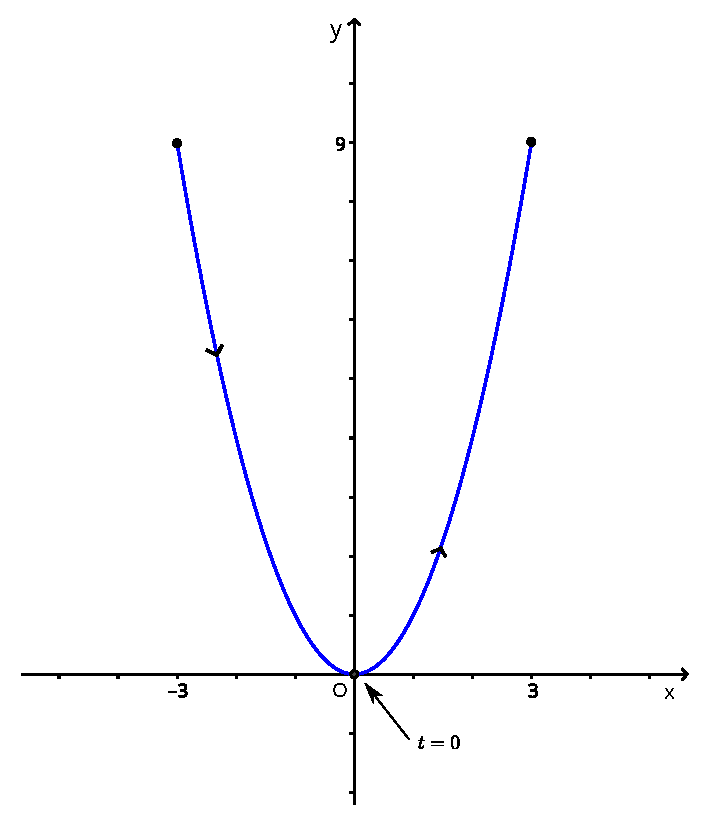
\includegraphics[width=0.4\textwidth]{parabola-teorie2.eps}
		      	\caption{Parabola \textit{k} pro $t \in \langle-3,3\rangle$}
		      \end{figure}
		      $$k(t)=[-t, t^2], t \in \langle-3,3\rangle$$
		      \begin{figure}[H]
		      	\centering
		      	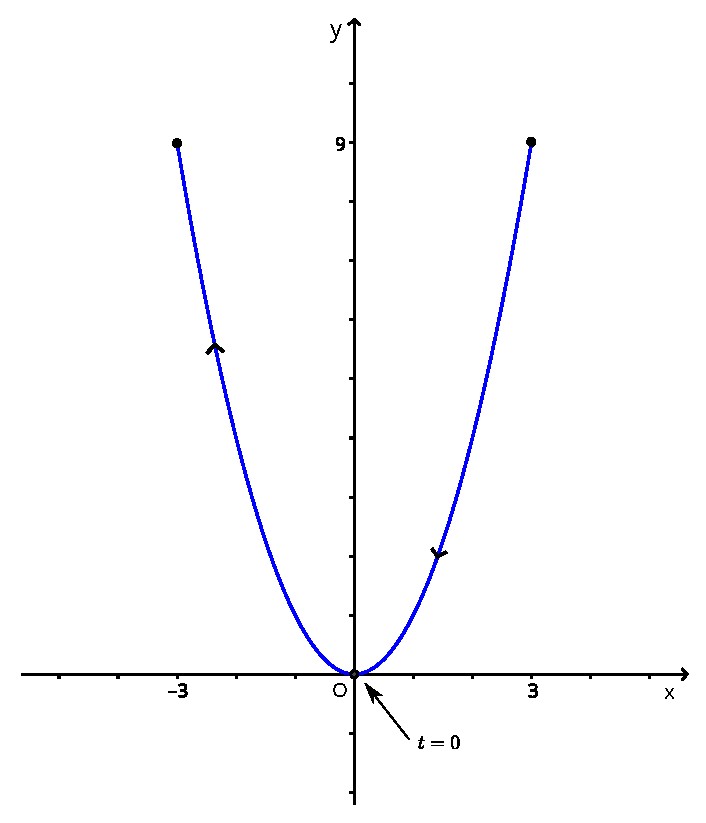
\includegraphics[width=0.4\textwidth]{parabola-teorie3.eps}
		      	\caption{Parabola \textit{k} pro $t \in \langle-3,3\rangle$}
		      \end{figure}
		      $$k(t)=[t+1, (t+1)^2], t \in \langle-3,3\rangle$$
		      \begin{figure}[H]
		      	\centering
		      	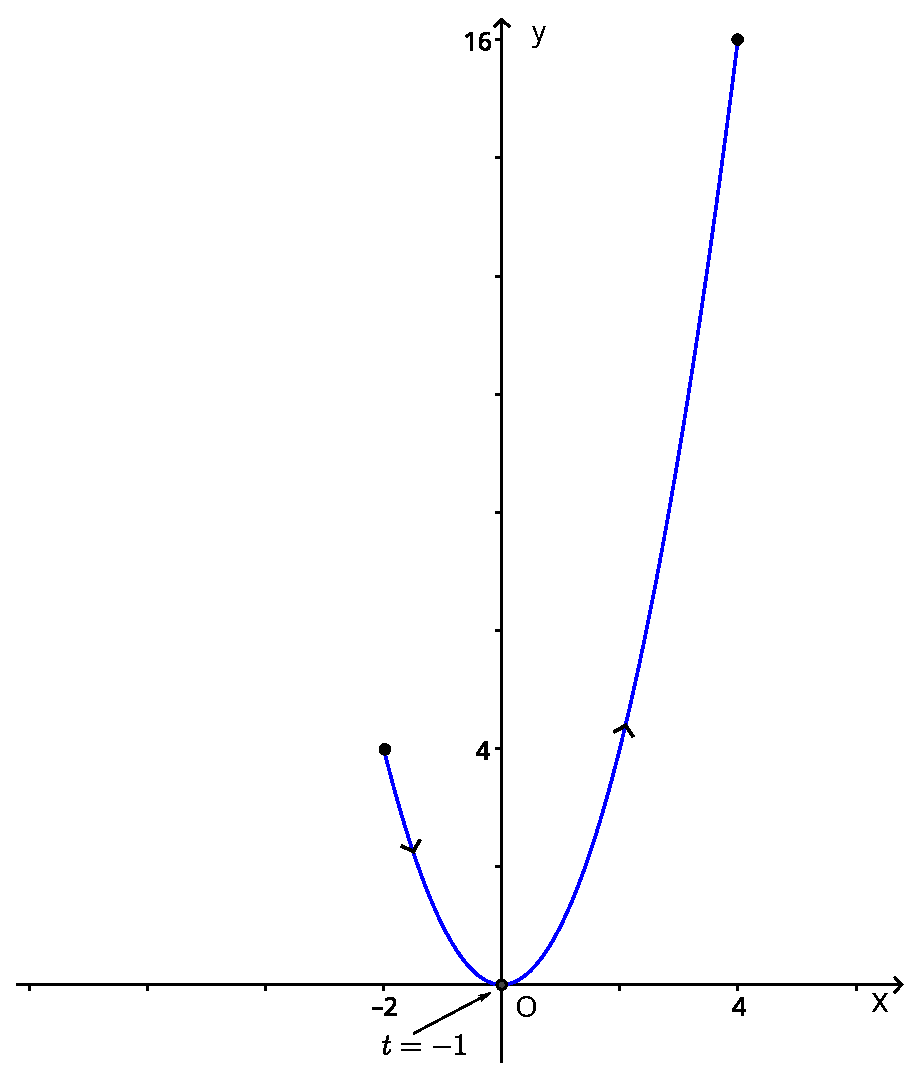
\includegraphics[width=0.4\textwidth]{parabola-teorie4.eps}
		      	\caption{Parabola \textit{k} pro $t \in \langle-3,3\rangle$}
		      \end{figure}
		      $$k(t)=[1-t, (1-t)^2], t \in \langle-3,3\rangle$$
		      \begin{figure}[H]
		      	\centering
		      	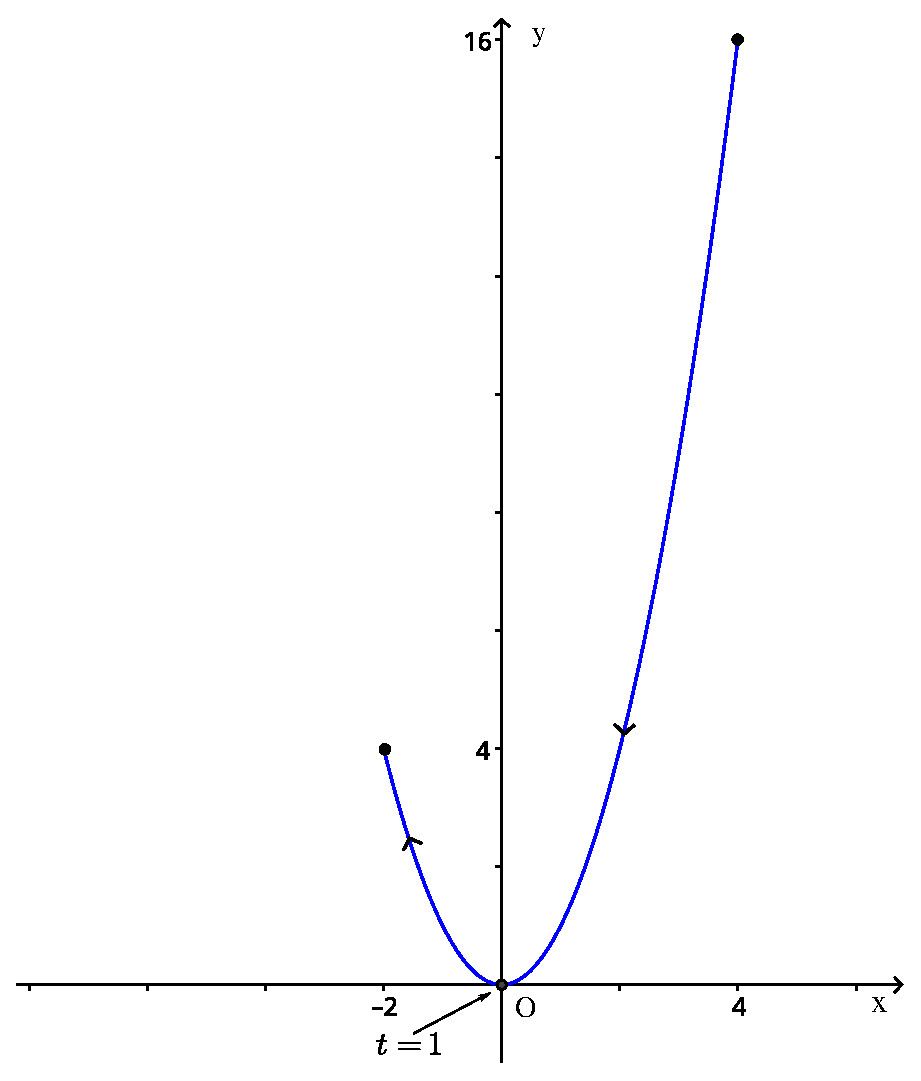
\includegraphics[width=0.4\textwidth]{parabola-teorie5.eps}
		      	\caption{Parabola \textit{k} pro $t \in \langle-3,3\rangle$}
		      \end{figure}
		      \clearpage
		      Podobně můžeme postupovat pro další paraboly \\
		      \begin{center}
		      	\begin{tabular}{ccc}
		      		$x^2=-2py$ & $x=t$, $t^2=-2py$ & $k(t)=\left[t, -\frac{t^2}{2p}\right], t \in \mathbb{R}$, \\ 
		      		$y^2=2px$  & $y=t$, $t^2=2px$  & $k(t)=\left[\frac{t^2}{2p}, t\right], t \in \mathbb{R}$,  \\ 
		      		$y^2=-2px$ & $y=t$, $t^2=-2px$ & $k(t)=\left[-\frac{t^2}{2p}, t\right], t \in \mathbb{R}$. 
		      	\end{tabular} 
		      \end{center}
		      V případě parabol s vrcholem $V=[m, n]$ volíme často parametrizaci tak, aby $k(0)=V$. Volbou intervalu pro parametr \textit{t} snadno vybereme požadovanou část paraboly.
		      Např. 
		      \begin{align*}
		      	(x-m)^2 = 2p(y-n),                                            \\
		      	t       = x-m,\quad x = t+m,                                  \\
		      	t^2     = 2p(y-n), \quad y = \frac{t^2}{2p}+n,                \\
		      	k(t)    = \left[t+m, \frac{t^2}{2p}+n\right], t\in\mathbb{R}, 
		      \end{align*}
		      \begin{align*}
		      	(y-n)^2 = -2p(x-m),                                            \\
		      	t       = y-n,\quad y = t+n,                                   \\
		      	t^2     = -2p(x-m),\quad  x = -\frac{t^2}{2p}+m,               \\
		      	k(t)    = \left[-\frac{t^2}{2p}+m, t+n\right], t\in\mathbb{R}. 
		      \end{align*}
		      \clearpage
		      \subsection*{Příklad 1}
		      Napište parametrické vyjádření paraboly zadané obecnou rovnicí
		      $$x^2-6x-10y+49=0.$$
		      Napište parametrické vyjádření části paraboly mezi jejími body \textit{P} a \textit{Q}, jejichž \textit{y}-ové
		      souřadnice jsou rovny $\frac{13}{2}$. \\[5pt]
		      \textbf{Řešení:}
		      \noindent\begin{enumerate}
		      \item Obecnou rovnici upravíme na vrcholový tvar
		      $$(x-3)^2=10(y-4).$$
		      Bod $V=[3,4]$ je vrchol, parametr $p=5$, ohnisko $F=\left[3,\frac{13}{2}\right]$,  řídící přímka $d: y=\frac{3}{2}$.
		      Volíme $t=x-3$, pak $t^2=10(y-4)$. Vypočítáme $x=t+3$, $y=\frac{t^2}{10}+4$.\\
		      Parametrické vyjádření paraboly je
		      $$k(t)=\left[t+3,\frac{t^2}{10}+4\right], t \in \mathbb{R}.$$
		      \vfill
		      \begin{figure}[H]
		      	\centering
		      	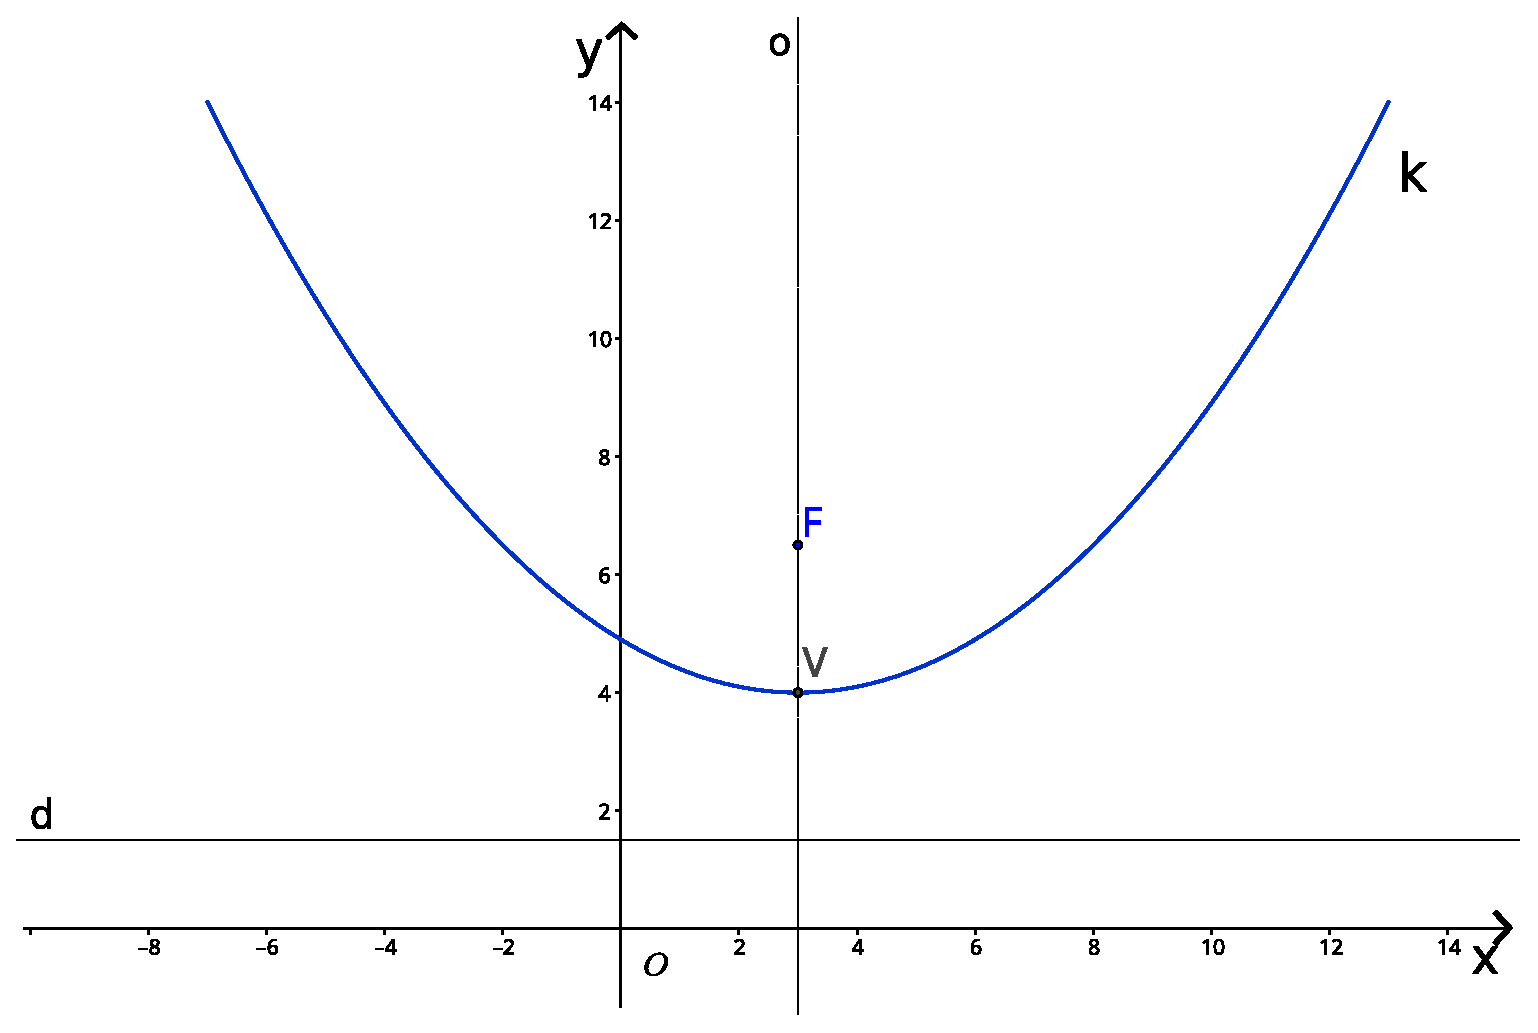
\includegraphics[width=0.8\textwidth]{parabola1.eps}
		      	\caption{Parabola pro $t \in \langle-10, 10\rangle$}
		      \end{figure}
		      				
		      \item
		      Souřadnice bodů \textit{P} a \textit{Q} můžeme vypočítat z obecné rovnice nebo z parametrického vyjádření
		      						
		      \noindent\begin{minipage}[t]{0.5\textwidth}
		      \begin{align*}
		      	x^2-6x-10\cdot\frac{13}{2}+49 & =0   \\
		      	x^2-6x-16                     & =0   \\
		      	x_1 = 8,\: x_2                & = -2 \\
		      	x = t+3,\: t                  & =x-3 \\
		      	t_1 = 5,\: t_2                & = -5 
		      \end{align*}
		\end{minipage}
		\begin{minipage}[t]{0.5\textwidth}
			\begin{align*}
				\frac{t^2}{10} + 4 & = \frac{13}{2}  \\
				\frac{t^2}{10}     & = \frac{5}{2}   \\
				t^2                & = 25            \\
				t_1                & = 5,\: t_2 = -5 
			\end{align*}
		\end{minipage}
		Pro parametr \textit{t} vybereme interval $\langle-5,5\rangle$, 
		\begin{align*}
			k(-5) & =\left[-2, \frac{13}{2}\right], \\
			k(5)  & =\left[8,\frac{13}{2}\right].   
		\end{align*}
		\end{enumerate}
		\vfill
		\begin{figure}[H]
			\centering
			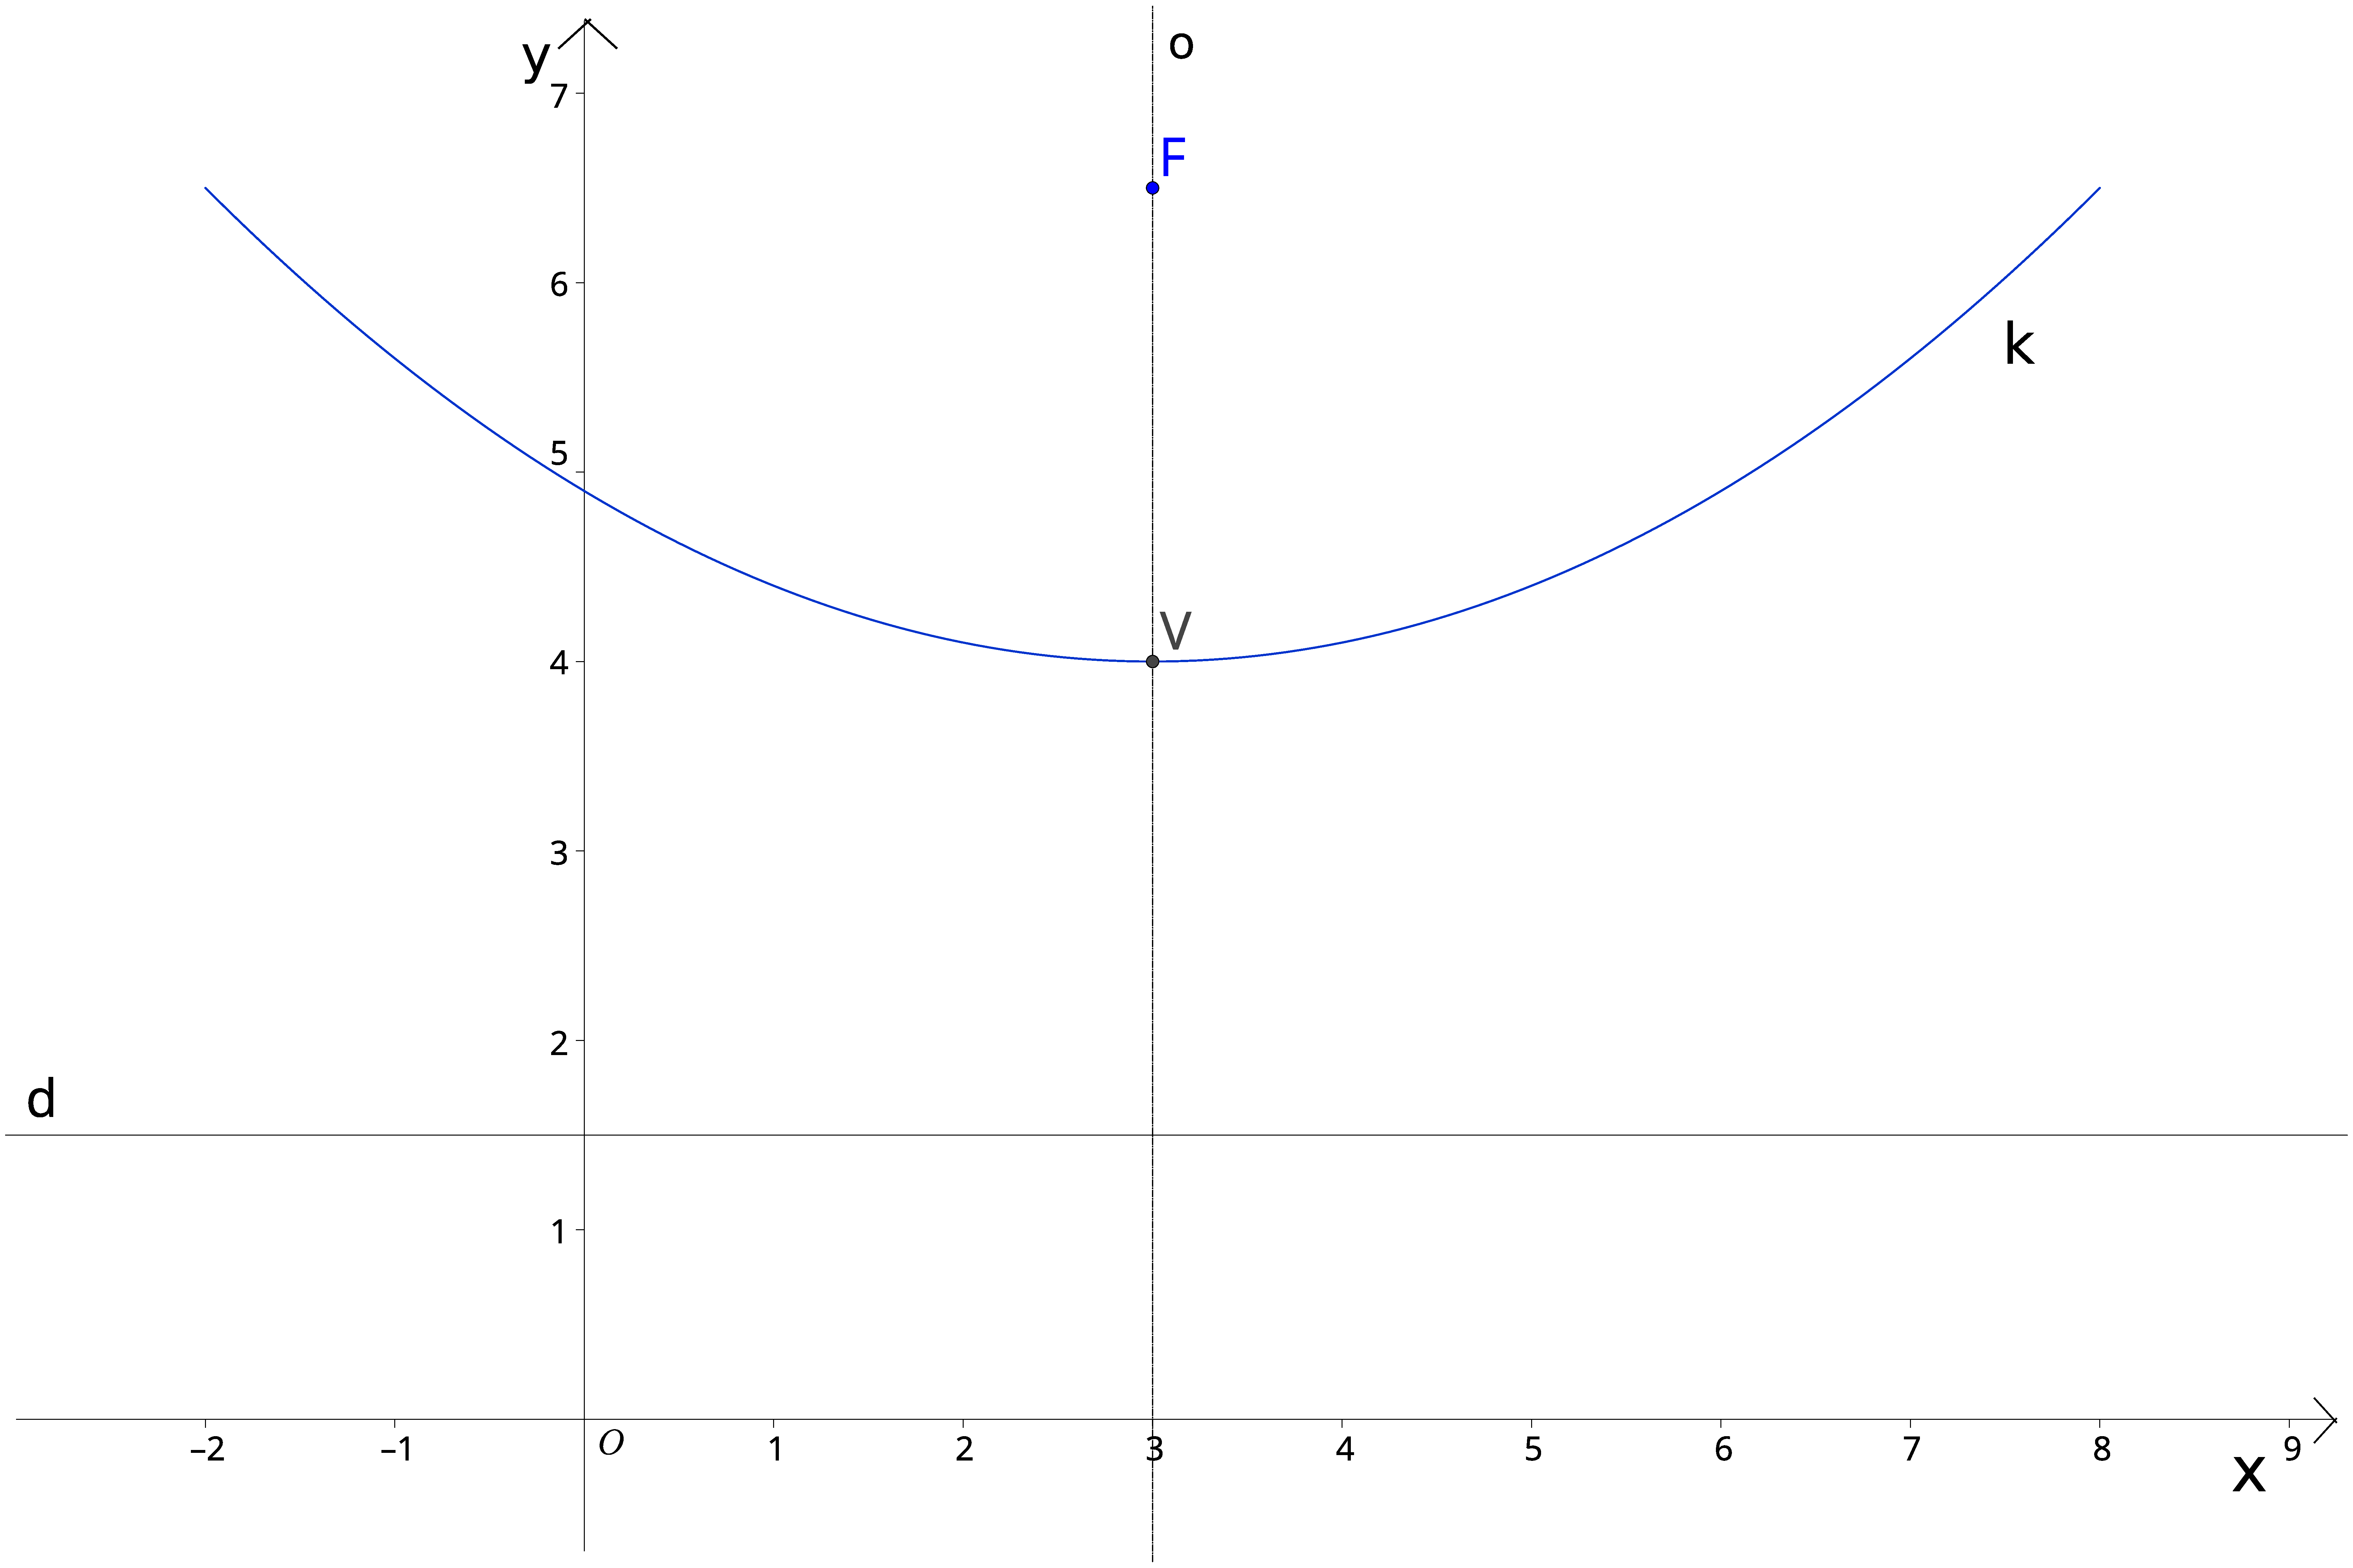
\includegraphics[width=0.9\textwidth]{parabola1-red.eps}
			\caption{Parabola pro $t \in \langle-5, 5\rangle$}					
		\end{figure}
		\clearpage
		\subsection*{Příklad 2}
		Napište parametrické vyjádření paraboly zadané obecnou rovnicí
		$$x^2-6x+10y-31=0.$$
		Napište parametrické vyjádření části paraboly mezi body \textit{P} a \textit{Q}, $x_P = -2$ a $x_Q = 13$.
		Parametrizaci volte tak, aby $k(0) = P$ a část paraboly byla probíhána směrem od bodu \textit{P} do bodu \textit{Q}. \\[5pt]
		\textbf{Řešení:}
		\noindent\begin{enumerate}
		\item Obecnou rovnici upravíme na vrcholový tvar
		$$(x-3)^2=-10(y-4).$$
		Bod $V=[3,4]$ je vrchol, parametr $p=5$, ohnisko $F=\left[3,\frac{3}{2}\right]$,  řídící přímka $d: y=\frac{13}{2}$.
		Volíme $t=x-3$, pak $t^2=-10(y-4)$. Vypočítáme $x=t+3$, $y=-\frac{t^2}{10}+4$.\\
		Parametrické vyjádření paraboly je
		$$k(t)=\left[t+3,-\frac{t^2}{10}+4\right], t \in \mathbb{R}.$$
		\vfill
		\begin{figure}[H]
			\centering
			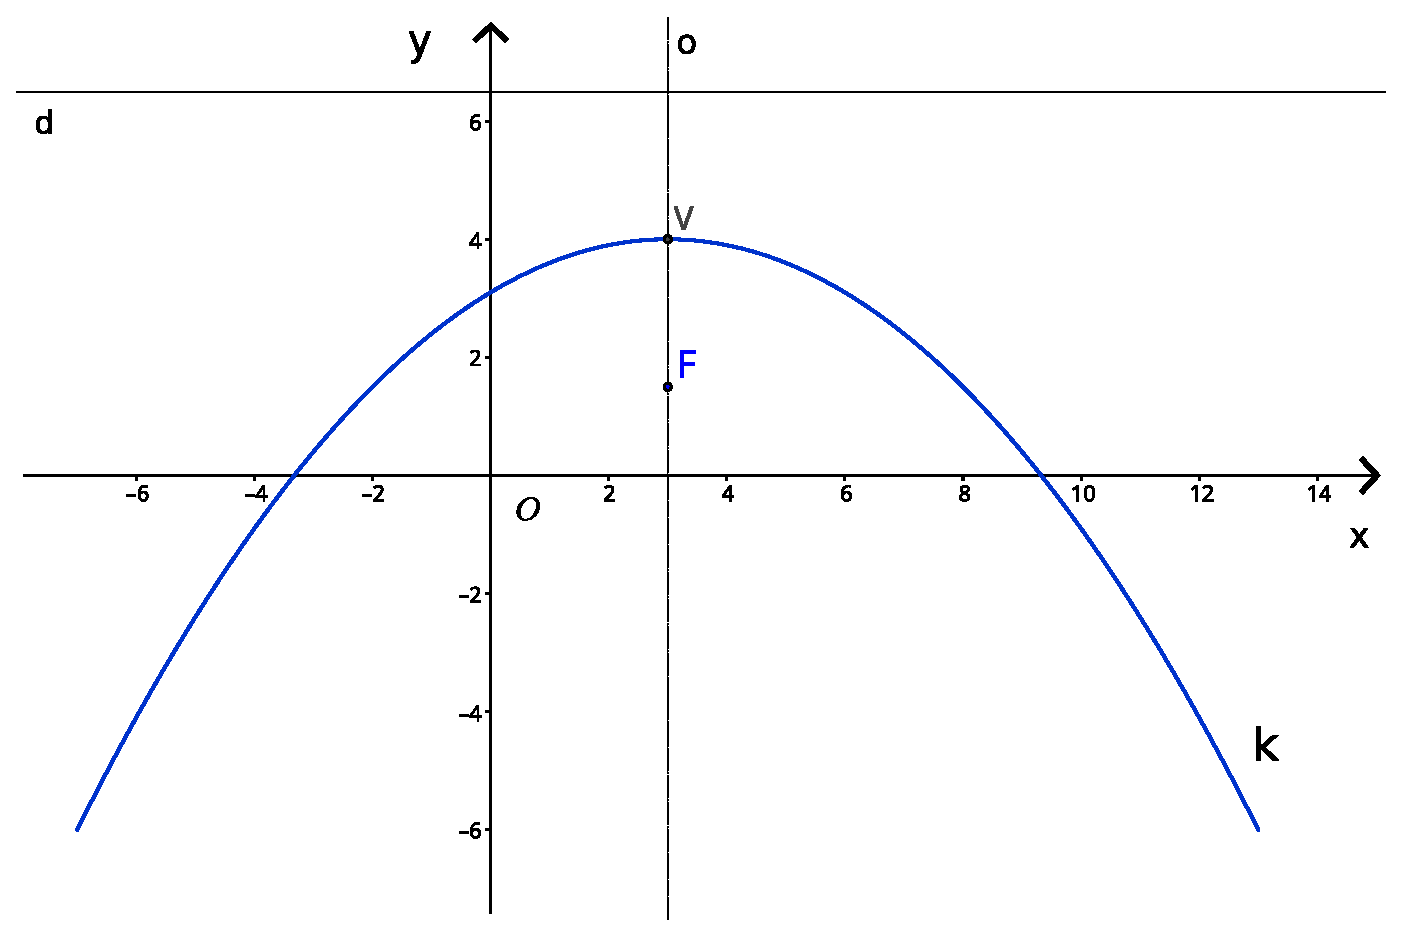
\includegraphics[width=0.8\textwidth]{parabola2.eps}
			\caption{Parabola pro $t \in \langle-10, 10\rangle$}
								
		\end{figure}
		\item
		Interval pro parametrizaci paraboly mezi body \textit{P} a \textit{Q} můžeme vypočítat například z parametrického vyjádření			
								
		\noindent\begin{minipage}[t]{0.5\textwidth}
		\begin{align*}
			t + 3 & = -2 \\
			t_1   & = -5 
		\end{align*}
		\end{minipage}
		\begin{minipage}[t]{0.5\textwidth}
			\begin{align*}
				t + 3 & = 13 \\
				t_2   & = 10 
			\end{align*}
		\end{minipage}
		\\[10pt]
		Daná parabola by tedy byla probíhaná z bodu \textit{P} do bodu \textit{Q} pro parametr \\ $t \in \langle-5, 10\rangle$.
		Aby bylo $k(0) = P$, změníme parametr $t = s - 5$ a máme:
		$$k(s)=\left[s-2,-\frac{(s-5)^2}{10}+4\right], s \in \langle0, 15 \rangle$$
		($s=t+5$, $s_1=-5+5=0$, $s_2=10+5=15$).
		\end{enumerate}
		\vfill
		\begin{figure}[H]
			\centering
			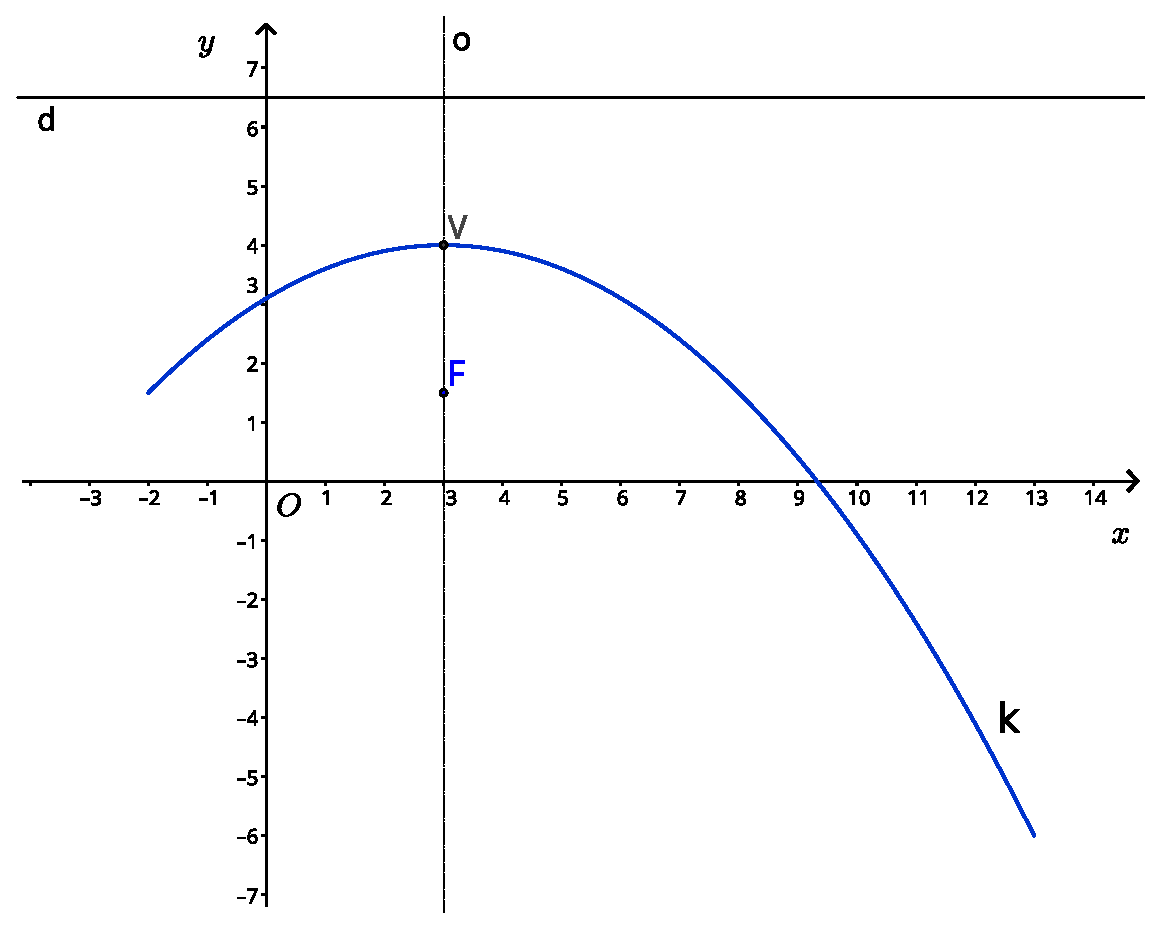
\includegraphics[width=0.9\textwidth]{parabola2-red.eps}
			\caption{Parabola pro $s \in \langle0, 15\rangle$}
								
		\end{figure}
		\clearpage
		\subsection*{Příklad 3}
		Napište parametrické vyjádření paraboly, bod $V=[3,4]$ je vrchol, osa paraboly je rovnoběžná s osou \textit{x} a bod $P=[13,14]$ je bodem paraboly.
		Napište parametrické vyjádření části paraboly mezi bodem \textit{P} a průsečíkem paraboly s osou \textit{x}. \\[5pt]
		\textbf{Řešení:}
		\noindent\begin{enumerate}
		\item Abychom mohli parabolu parametricky vyjádřit, nejdříve napíšeme vrcholový tvar rovnice paraboly.
		Parabola má rovnici $(y-n)^2=2p(x-m)$.
		Dosazením bodů \textit{V}\\ a \textit{P} získáme parametr \textit{p}:
		\begin{align*}
			(14-4)^2 & = 2p(13-3), \\
			100      & = 20p,      \\
			p        & = 5.        
		\end{align*}
		Obecná rovnice paraboly je tedy
		$$(y-4)^2=10(x-3).$$
		Parametr je $p=5$, ohnisko $F=\left[\frac{11}{2},4\right]$,  řídící přímka $d: x=\frac{1}{2}$.\\
		Volíme $t=y-4$, pak $t^2=10(x-3)$. Vypočítáme $x=\frac{t^2}{10}+3$, $y=t+4$.\\
		Parametrické vyjádření paraboly je
		$$k(t) = \left[\frac{t^2}{10}+3, t+4\right], t \in \mathbb{R}.$$
		\vfill
		\begin{figure}[H]
			\centering
			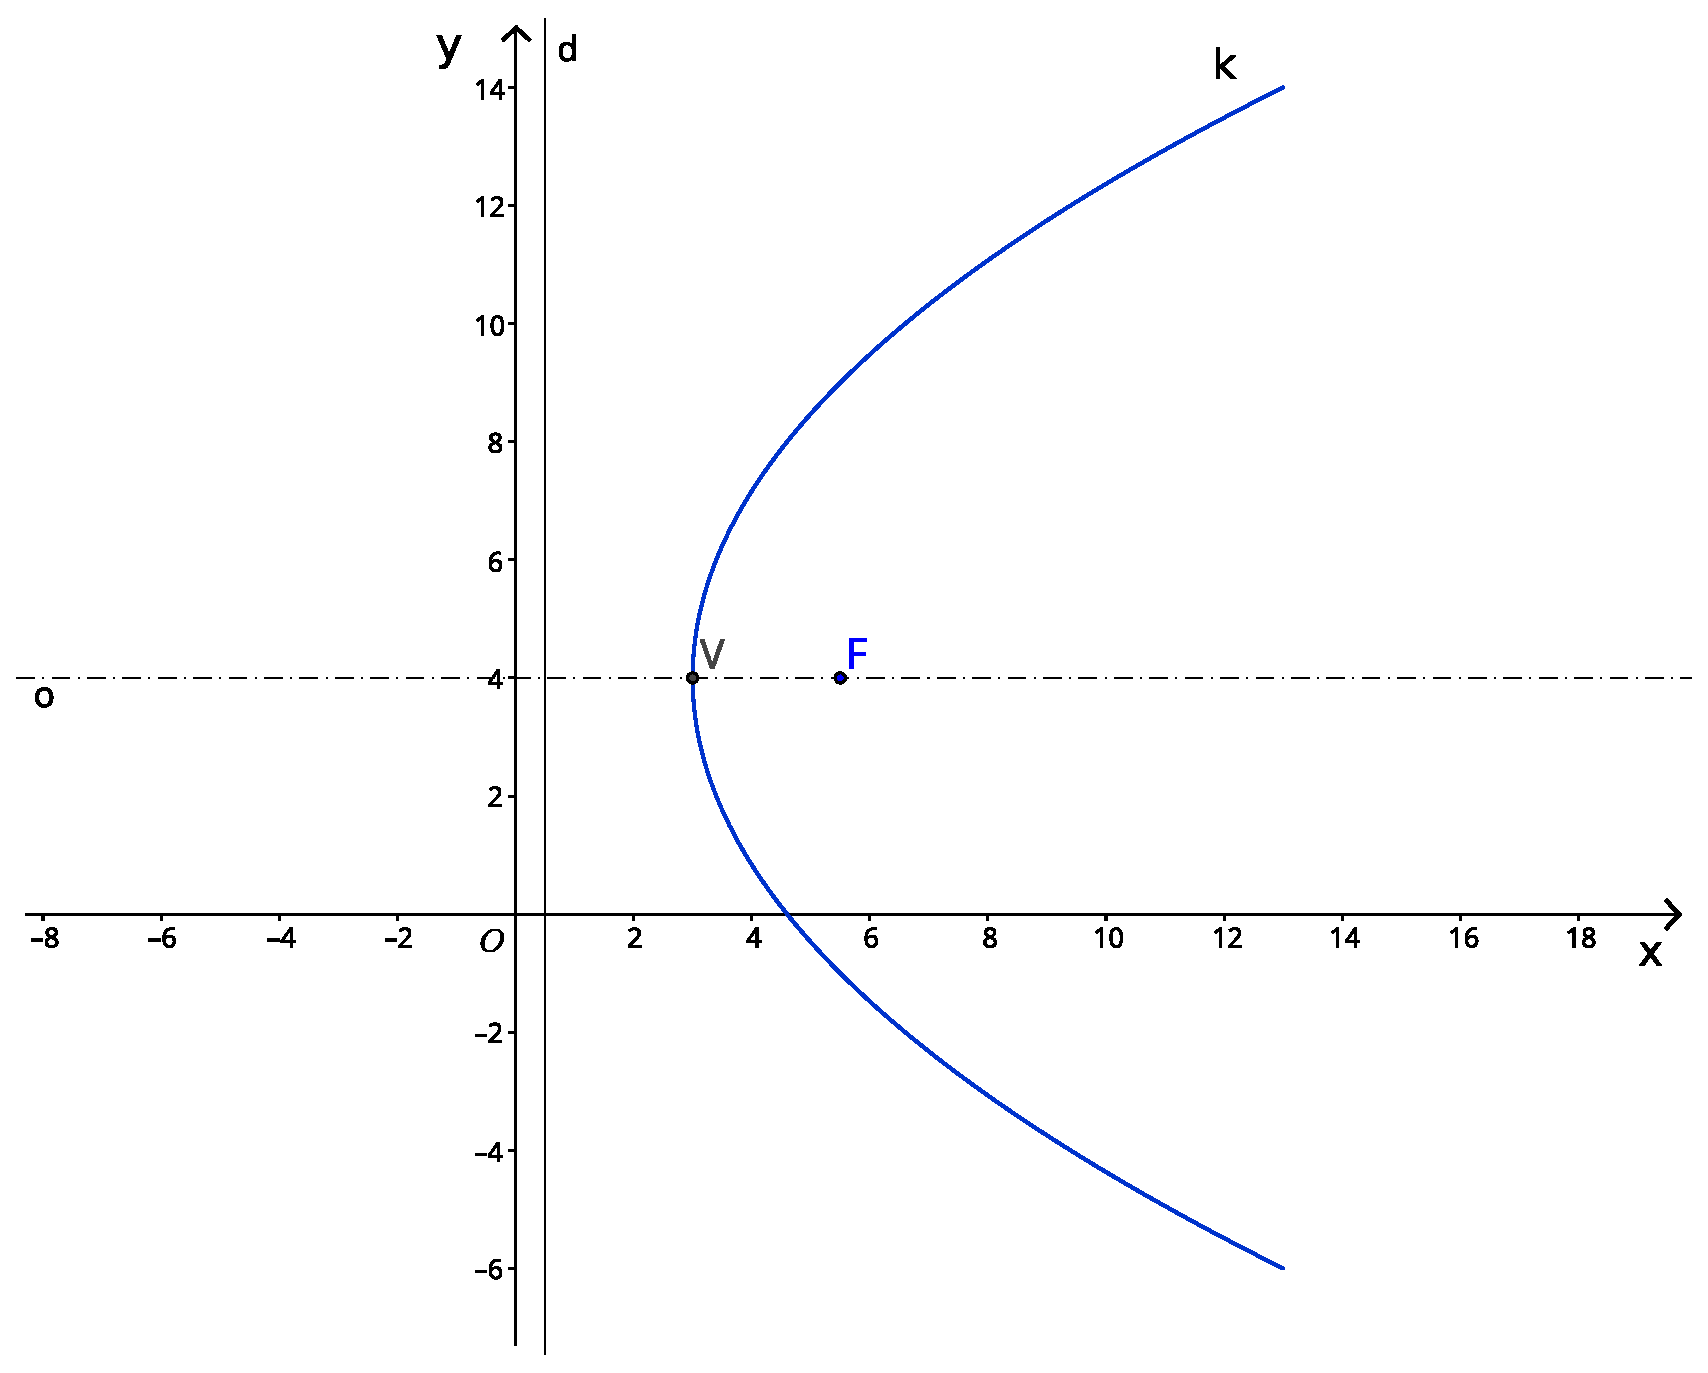
\includegraphics[width=0.5\textwidth]{parabola3.eps}
			\caption{Parabola pro $t \in \langle-10, 10\rangle$}
								
		\end{figure}
		\item
		Hodnoty parametru \textit{t} pro požadovanou část paraboly získáme z rovnic		
									
		\noindent\begin{minipage}[t]{0.5\textwidth}
		\begin{align*}
			t + 4 & = 0 \text{ (průsečík s osou \textit{x})} \\
			t_1   & = -4                                        
		\end{align*}
		\end{minipage}
		\noindent\begin{minipage}[t]{0.5\textwidth}
		\begin{align*}
			t + 4 & = 14 \text{ (bod \textit{P})} \\
			t_2   & = 10                          
		\end{align*}
		\end{minipage}
		\\[10pt]
		Část paraboly mezi bodem \textit{P} a průsečíkem s osou \textit{x} má parametrické vyjádření
		$$k(t) = \left[\frac{t^2}{10}+3, t+4\right], t \in \langle-4, 10\rangle.$$
		\end{enumerate}
		\vfill
		\begin{figure}[H]
			\centering
			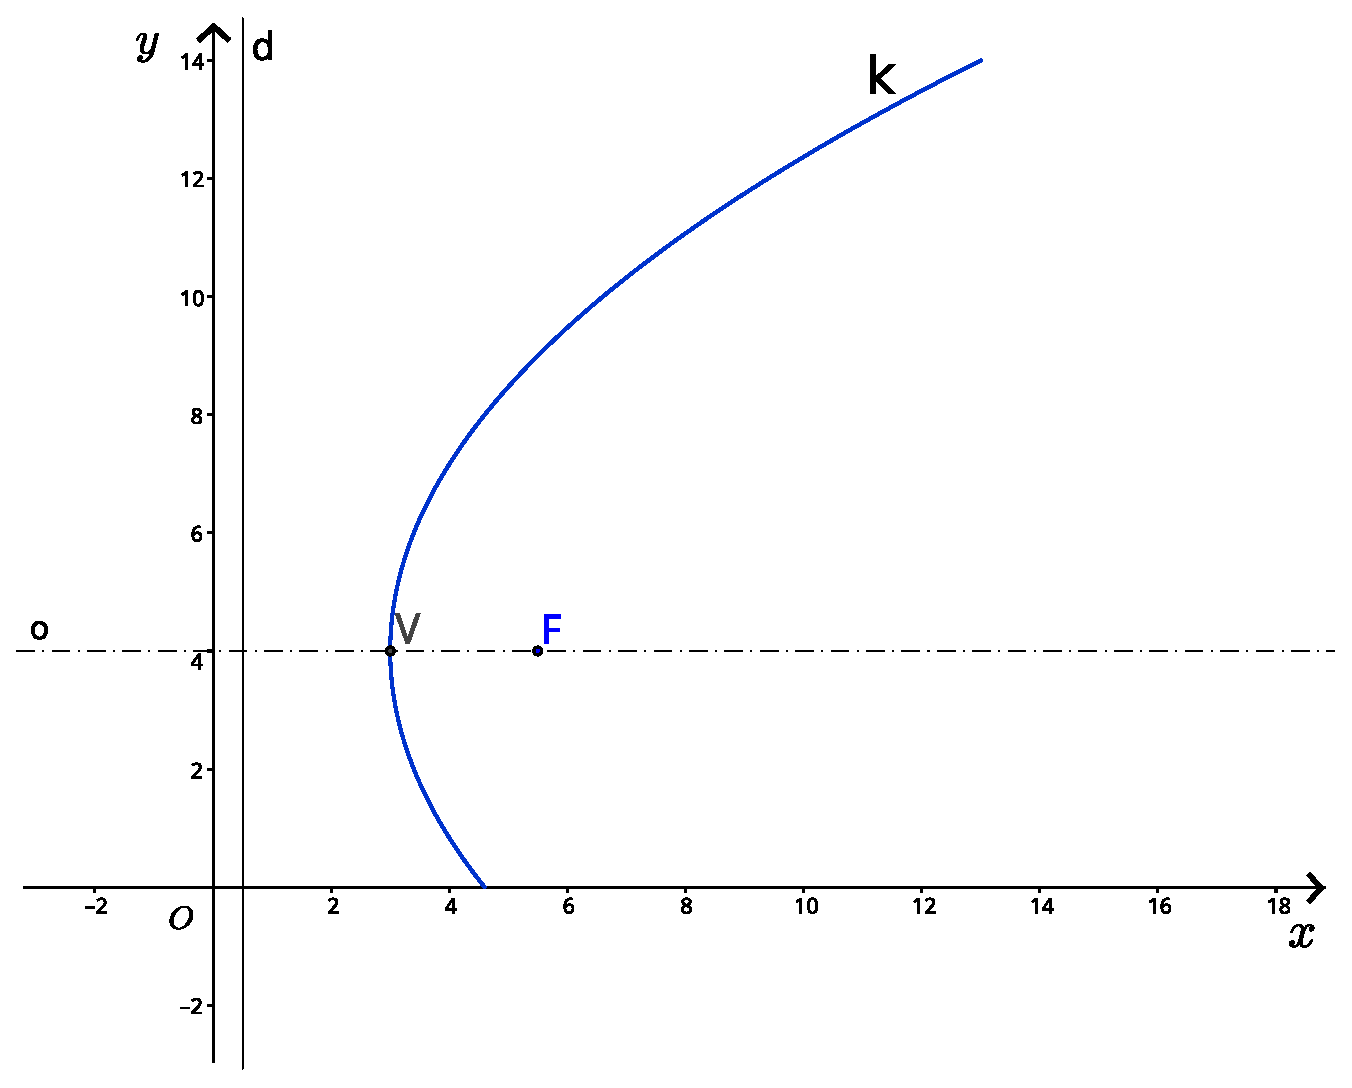
\includegraphics[width=0.9\textwidth]{parabola3-red.eps}
			\caption{Parabola pro $t \in \langle-4, 10\rangle$}
								
		\end{figure}
		\clearpage
		\subsection*{Příklad 4}
		Napište parametrické vyjádření paraboly, bod $F=\left[\frac{1}{2}, 4\right]$ je ohnisko, obecná rovnice
		řídící přímky \textit{d} je $x=\frac{11}{2}$. \\
		Napište parametrické vyjádření části paraboly mezi průsečíkem \textit{P} paraboly s osou \textit{x} a průsečíkem
		\textit{Q} paraboly s osou \textit{y}, $y_Q>0$. \\[5pt]
		\textbf{Řešení:}
		\noindent\begin{enumerate}
		\item Abychom mohli parabolu parametricky vyjádřit, nejdříve napíšeme vrcholový tvar rovnice paraboly.
		Protože řídící přímka je rovnoběžná s osou \textit{y}, je osa paraboly rovnoběžná s osou \textit{x}.
		Parametr \textit{p} je vzdálenost ohniska \textit{F} od řídící přímky \textit{d}, $p=5$. Snadno zjistíme i vrchol $V=[3,4]$. \\
		Parabola má vrcholovou rovnici $(y-n)^2=-2p(x-m)$.
		Po dosazení konkrétních hodnot nám vyjde
		$$(y-4)^2=-10(x-3).$$
		Volíme $t=y-4$, pak $t^2=-10(x-3)$. Vypočítáme $x=-\frac{t^2}{10}+3$, $y=t+4$.\\
		Parametrické vyjádření paraboly je
		$$k(t) = \left[-\frac{t^2}{10}+3, t+4\right], t \in \mathbb{R}.$$
		\vfill
		\begin{figure}[H]
			\centering
			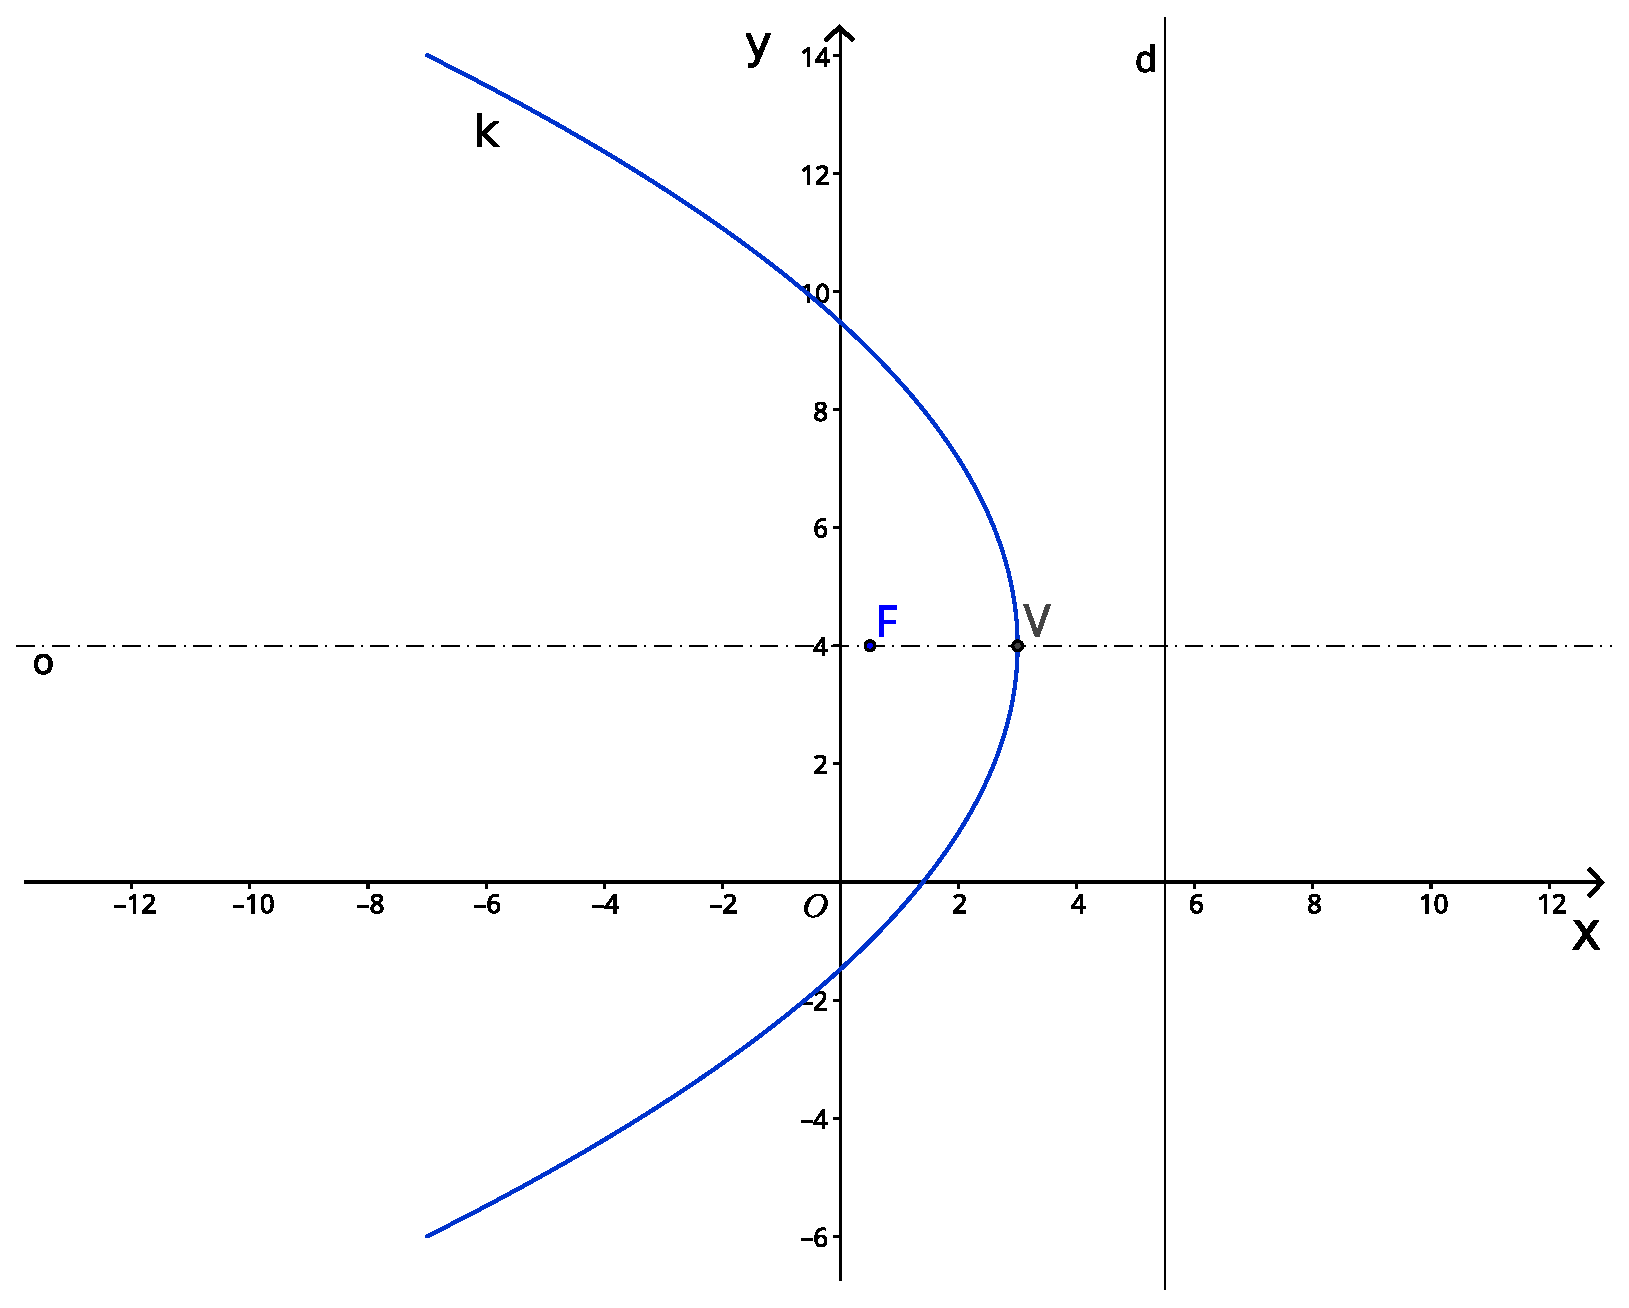
\includegraphics[width=0.7\textwidth]{parabola4.eps}
			\caption{Parabola pro $t \in \langle-10, 10\rangle$}
								
		\end{figure}
		\item
		Hodnoty parametru \textit{t} pro požadovanou část paraboly získáme z rovnic
									
		\noindent\begin{minipage}[t]{0.5\textwidth}
		\begin{align*}
			t + 4 & = 0 \text{ (průsečík s osou \textit{x})} \\
			t_1   & = -4                                        
		\end{align*}
		\end{minipage}
		\noindent\begin{minipage}[t]{0.5\textwidth}
		\begin{align*}
			-\frac{t^2}{10}+3 & = 0 \text{ (bod \textit{Q})} \\
			t^2               & = 30                         \\
			t_2               & = \sqrt{30} \quad (y_Q>0)    
		\end{align*}
		\end{minipage}
		\\[10pt]
		Část paraboly mezi průsečíky \textit{P} a \textit{Q} má vyjádření
		$$k(t) = \left[-\frac{t^2}{10}+3, t+4\right], t \in \langle-4, \sqrt{30}\rangle.$$
		\end{enumerate}
		\vfill
		\begin{figure}[H]
			\centering
			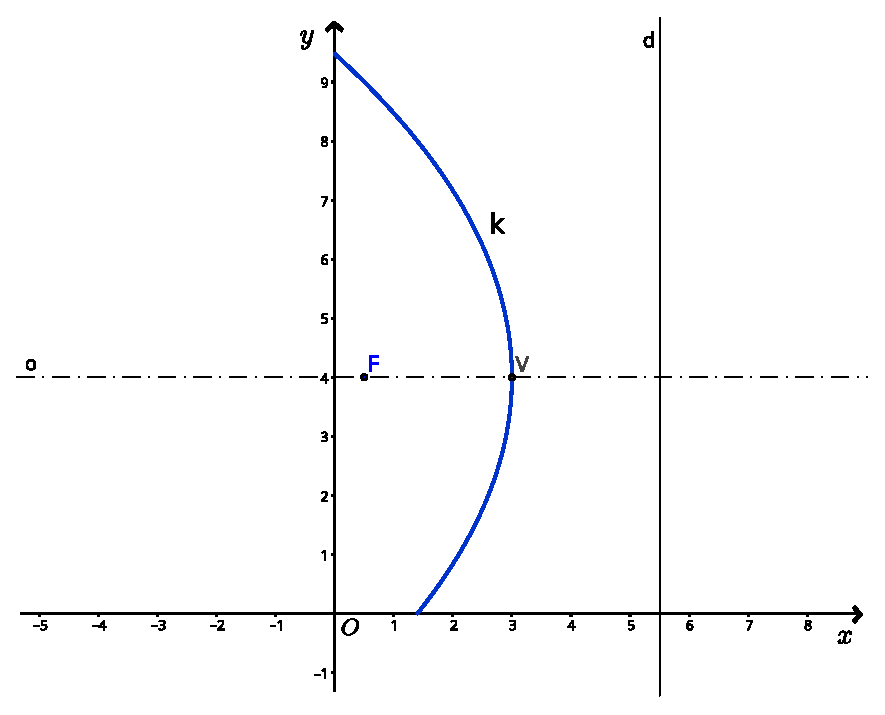
\includegraphics[width=0.9\textwidth]{parabola4-red.eps}
			\caption{Parabola pro $t \in \langle-4, \sqrt{30}\rangle$}
								
		\end{figure}
		\clearpage		
		\section{Elipsa}
		Kružnice je speciální případ elipsy. Dá se předpokládat, že parametrizace elipsy bude podobná parametrizaci kružnice. \\
		Uvažujme nejprve elipsu o středu $O=[0,0]$, velikost hlavní poloosy značíme \textit{a}, velikost vedlejší poloosy
		značíme \textit{b}. Platí $a > b$. \\
		Rovnice elipsy ve středovém tvaru je pak
		$$\frac{x^2}{a^2}+\frac{y^2}{b^2}=1$$
		a hlavní osa elipsy je osa \textit{x}, nebo
		$$\frac{x^2}{b^2}+\frac{y^2}{a^2}=1$$
		a hlavní osa elipsy je osa \textit{y}. \\
		Pro parametrizaci elipsy použijeme vzorec
		$$\cos^2{t}+\sin^2{t}=1.$$
		Pro rovnici $\frac{x^2}{a^2}+\frac{y^2}{b^2}=1$ dáme do rovnosti $\frac{x}{a}=\cos{t}$ a $\frac{y}{b}=\sin{t}$
		(popř. $\frac{x}{a}=\sin{t}$ a $\frac{y}{b}=\cos{t}$). \\
		Parametrický popis elipsy je
		$$k(t)=[a\cos{t}, b\sin{t}]$$
		(popř. $k(t)=[a\sin{t}, b\cos{t}]$), pro jeden oběh bereme $t \in \langle0, 2\pi\rangle$. \\
		Pro rovnici $\frac{x^2}{b^2}+\frac{y^2}{a^2}=1$ dáme do rovnosti $\frac{x}{b}=\cos{t}$ a $\frac{y}{a}=\sin{t}$
		(popř. $\frac{x}{b}=\sin{t}$ a $\frac{y}{a}=\cos{t}$). \\
		Parametrický popis elipsy je
		$$k(t)=[b\cos{t}, a\sin{t}]$$
		(popř. $k(t)=[b\sin{t}, a\cos{t}]$), $t \in \langle0, 2\pi\rangle$. \\
		Snadno ověříme: je-li funkce $\cos$ v \textit{x}-ové souřadnici, výchozí bod $k(0)$ je vrchol na ose \textit{x}, je-li
		funkce $\cos$ v \textit{y}-ové souřadnici, je výchozí bod $k(0)$ vrchol elipsy na ose \textit{y}. \\
		Pro obecnější případ, kdy střed elipsy je bod $S=[m, n]$ a rovnice ve středovém tvaru je
		$$\frac{(x-m)^2}{a^2}+\frac{(y-n)^2}{b^2}=1$$
		nebo
		$$\frac{(x-m)^2}{b^2}+\frac{(y-n)^2}{a^2}=1,$$
		změníme předchozí parametrický popis přičtením vektoru posunutí $S-O=(m,n)$, tedy
		$$k(t)=[m+a\cos{t}, n+b\sin{t}]$$
		(popř. $k(t)=[m+a\sin{t}, n+b\cos{t}]$) \\
		nebo
		$$k(t)=[m+b\cos{t}, n+a\sin{t}].$$
		(popř. $k(t)=[m+b\sin{t}, n+a\cos{t}]$) \\			
		$t \in \langle0, 2\pi\rangle$ pro 1 oběh. \\[10pt]
		Změnou znaménka u funkce $\cos$ měníme výchozí vrchol elipsy, změnou znaménka u funkce $\sin$ měníme směr probíhání elipsy. \\
		Otázka je, zda můžeme vybrat za výchozí bod jiný bod elipsy než vrchol. To je možné, ale museli bychom brát v úvahu sdružené
		průměry elipsy, nebylo by to tak jednoduché jako u kružnice. Tímto se v textu zabývat nebudeme. \\[10pt]
		V této části si ukážeme, jak jednoduše můžeme popsat tečny parametricky zadaných křivek. \\
		Mějme křivku $k(t)=[x(t), y(t)]$, $t \in I$(interval), vybereme si bod na této křivce $K=k(t_0)$ ($t_0$ je vybrané číslo z intervalu \textit{I}).
		Tečna křivky souvisí s derivací, u parametricky zadaných křivek derivujeme zvlášť každou souřadnici a značíme
		$$k'(t)=(x'(t), y'(t)), t \in I.$$
		To jsou tečné vektory křivky \textit{k}. \\
		Tečný vektor v bodě $K=k(t_0)$ je vektor
		$$k'(t_0)=(x'(t_0), y'(t_0)).$$
		Velikost tohoto vektoru vypovídá navíc o rychlosti, jakou je křivka v daném bodě probíhána. Tečna křivky \textit{k} v bodě \textit{K}
		je určena bodem $K=k(t_0)$ a směrovým vektorem $k'(t_0)$.
		\clearpage
		\subsection*{Příklad 1}
		\noindent Napište parametrické vyjádření elipsy zadané obecnou rovnicí
		$$9x^2+16y^2-72x-96y=0.$$
		Dále napište souřadnice průsečíků se souřadnicovými osami a napište obecné rovnice tečen elipsy v těchto  průsečících. \\[10pt]
		\textbf{Řešení:} Obecnou rovnici upravíme na středový tvar
		$$\frac{(x-4)^2}{32}+\frac{(y-3)^2}{18}=1.$$
		Střed elipsy je bod $S=[4,3]$, hlavní osa je rovnoběžná s osou \textit{x}, velikost hlavní poloosy je $a=4\sqrt{2}$,
		velikost vedlejší poloosy $b=3\sqrt{2}$. \\
		Dáme do rovnosti např.
		\begin{align*}
			\frac{x-4}{4\sqrt{2}} & = \cos{t},  \\
			\frac{y-3}{3\sqrt{2}} & = \sin{t} . 
		\end{align*}
		a máme parametrické vyjádření
		$$k(t) = [4+4\sqrt{2} \cdot \cos{t}, 3+3\sqrt{2} \cdot \sin{t}], t\in\langle0,2\pi\rangle.$$
		Výchozí bod je bod $k(0) = [4+4\sqrt{2},3]$, což je pravý hlavní vrchol. Protože $k\left(\frac{\pi}{2}\right) = [4, 3+3\sqrt{2}]$
		je horní vedlejší vrchol, je elipsa probíhána v kladném směru. Souřadnice průsečíků se souřadnicovými osami
		můžeme určit z obecné rovnice nebo z parametrického vyjádření:
		\begin{enumerate}
			\item průsečíky s osou \textit{x} ($y=0$)
			      				      			
			      \noindent\begin{minipage}[t]{0.5\textwidth}
			      \begin{align*}
			      	9x^2-72x & = 0 \\
			      	9x(x-8)  & = 0 \\
			      	x_1      & = 0 \\
			      	x_2      & = 8 \\
			      \end{align*}
			      Průsečíky s osou \textit{x} jsou body $P_1=[0,0]$ a $P_2=[8,0]$.
			\end{minipage}
			nebo
			\noindent\begin{minipage}[t]{0.5\textwidth}
			\begin{align*}
				3+3\sqrt{2}\sin{t}              & = 0                           \\
				\sin{t}                         & = -\frac{\sqrt{2}}{2}         \\
				t_1                             & = \frac{5\pi}{4}              \\
				t_2                             & = \frac{7\pi}{4}              \\
				\text{(vybíráme řešení v } & \langle0, 2\pi\rangle\text{)} \\
				k\left(\frac{5\pi}{4}\right)    & = [0, 0]                      \\
				k\left(\frac{7\pi}{4}\right)    & = [8, 0]                      
			\end{align*}
			\end{minipage}		
			\item průsečíky s osou \textit{y} ($x=0$)
			      				      			
			      \noindent\begin{minipage}[t]{0.5\textwidth}
			      \begin{align*}
			      	16y^2-96y & = 0 \\
			      	16y(y-6)  & = 0 \\
			      	y_1       & = 0 \\
			      	y_2       & = 6 \\
			      \end{align*}
			      Průsečíky s osou \textit{y} jsou body $P_1=[0,0]$ a $P_3=[0,6]$.
			\end{minipage}
			\noindent\begin{minipage}[t]{0.5\textwidth}
			\begin{align*}
				4+4\sqrt{2}\cos{t}           & = 0                   \\
				\cos{t}                      & = -\frac{\sqrt{2}}{2} \\
				t_1                          & = \frac{5\pi}{4}      \\
				t_3                          & = \frac{3\pi}{4}      \\
				k\left(\frac{5\pi}{4}\right) & = [0, 0]              \\
				k\left(\frac{3\pi}{4}\right) & = [0, 6]              
			\end{align*}
			\end{minipage}	
		\end{enumerate}
		Nyní vypočítáme tečné vektory:
		$$k'(t) = (-4\sqrt{2} \cdot \sin{t}, 3\sqrt{2} \cdot \cos{t}).$$
		V bodě $k\left(\frac{5\pi}{4}\right) = [0,0]$ je tečný vektor $k'\left(\frac{5\pi}{4}\right) = (4,-3)$
		a obecná rovnice tečny je \\ $p_1: 3x+4y=0$. \\
		V bodě $k\left(\frac{3\pi}{4}\right) = [0,6]$ je tečný vektor $k'\left(\frac{3\pi}{4}\right) = (-4,-3)$
		a obecná rovnice tečny je \\ $p_3: 3x-4y+24=0$. \\
		V bodě $k\left(\frac{7\pi}{4}\right) = [8,0]$ je tečný vektor $k'\left(\frac{7\pi}{4}\right) = (4,3)$
		a obecná rovnice tečny je \\ $p_2: 3x-4y-24=0$. \\
		Poslední dvě tečny jsou rovnoběžné.
		\vfill
		\begin{figure}[H]
			\centering
			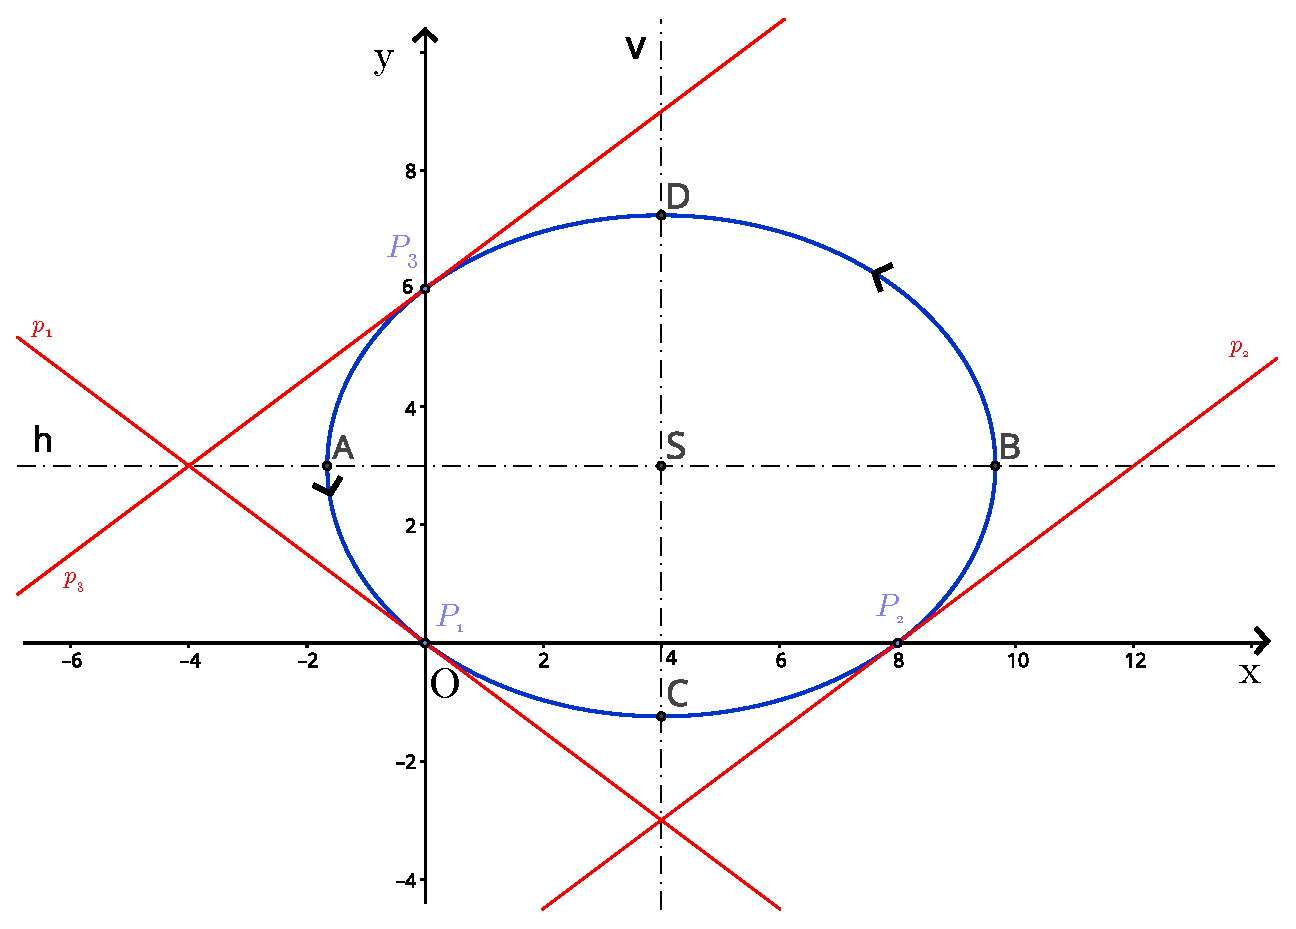
\includegraphics[width=0.9\textwidth]{elipsa1.eps}
			\caption{Elipsa pro $t \in \langle0, 2\pi\rangle$}
								
		\end{figure}
		\clearpage				
		\subsection*{Příklad 2}
		Napište parametrické vyjádření elipsy, body $E=[3,4+\sqrt{14}]$ a $F=[3,4-\sqrt{14}]$ jsou její ohniska,
		velikost vedlejší poloosy $b=3\sqrt{2}$ \\
		Elipsu parametrizujte tak, aby výchozí bod $k(0)$ byl levý vedlejší vrchol a elipsa byla probíhána v kladném směru. \\
		Napište obecné rovnice normál elipsy v jejich průsečících se souřadnými osami. \\
		\textbf{Poznámka:} Normála křivky v bodě \textit{K} je přímka kolmá k tečně v tomto bodě \textit{K}. \\[10pt]
		\textbf{Řešení:} Ze zadaných ohnisek snadno získáme excentricitu $e=\sqrt{14}$ a pomocí vztahu $a^2=e^2+b^2$
		dopočítáme velikost hlavní poloosy $a=4\sqrt{2}$. Střed leží ve středu úsečky $EF$ a jeho souřadnice jsou tedy $S=[3,4]$.\\
		Hlavní osa je rovnoběžná s osou \textit{y}. Vypočítané hodnoty použijeme
		pro napsání středového tvaru obecné rovnice elipsy:
		$$\frac{(x-m)^2}{b^2}+\frac{(y-n)^2}{a^2}=1,$$
		$$\frac{(x-3)^2}{18}+\frac{(y-4)^2}{32}=1.$$
		Pro parametrizaci dáme do rovnosti např.:
		\begin{align*}
			\frac{x-3}{3\sqrt{2}} & = \cos{t}, \\
			\frac{y-4}{4\sqrt{2}} & = \sin{t}. 
		\end{align*}
		a máme parametrické vyjádření
		$$k(t) = [3+3\sqrt{2} \cdot \cos{t}, 4+4\sqrt{2} \cdot \sin{t}], t\in\langle0,2\pi\rangle.$$
		Výchozí bod je bod $k(0) = [3+3\sqrt{2},4]$, což je pravý vedlejší vrchol. Abychom napsali vyjádření s výchozím bodem v
		levém vedlejším vrcholu, změníme znaménko u funkce $\cos$. Protože je $k\left(\frac{\pi}{2}\right)=[3,4+4\sqrt{2}]$, je elipsa probíhána v záporném směru. Změníme tedy i znaménko u funkce $\sin$. \\ Požadované parametrické vyjádření elipsy je pak
		$$k(t) = [3-3\sqrt{2} \cdot \cos{t}, 4-4\sqrt{2} \cdot \sin{t}], t\in\langle0,2\pi\rangle.$$
		Souřadnice průsečíků se souřadnicovými osami
		můžeme určit například z parametrického vyjádření:
		\clearpage
		\begin{enumerate}
			\item průsečíky s osou \textit{x} ($y=0$)
			      				      		
			      \begin{align*}
			      	4-4\sqrt{2}\sin{t}              & = 0                           \\
			      	\sin{t}                         & = \frac{\sqrt{2}}{2}          \\
			      	t_1                             & = \frac{\pi}{4}               \\
			      	t_2                             & = \frac{3\pi}{4}              \\
			      	\text{(vybíráme řešení v } & \langle0, 2\pi\rangle\text{)} \\
			      	k\left(\frac{\pi}{4}\right)     & = [0, 0] = P_1                \\
			      	k\left(\frac{3\pi}{4}\right)    & = [6, 0] = P_2                
			      \end{align*}
			      				      			
			\item průsečíky s osou \textit{y} ($x=0$)
			      				      			
			      \begin{align*}
			      	3-3\sqrt{2}\cos{t}           & = 0                  \\
			      	\cos{t}                      & = \frac{\sqrt{2}}{2} \\
			      	t_1                          & = \frac{\pi}{4}      \\
			      	t_3                          & = \frac{7\pi}{4}     \\
			      	k\left(\frac{\pi}{4}\right)  & = [0, 0] = P_1       \\
			      	k\left(\frac{7\pi}{4}\right) & = [0, 8] = P_3       
			      \end{align*}
		\end{enumerate}
		Nyní vypočítáme tečné vektory
		$$k'(t) = (3\sqrt{2} \cdot \sin{t}, -4\sqrt{2} \cdot \cos{t})$$
		V bodě $k\left(\frac{\pi}{4}\right) = [0,0]$ je tečný vektor $k'\left(\frac{\pi}{4}\right) = (3,-4)$
		a obecná rovnice normály je \\ $n_1: 3x-4y=0$. \\
		V bodě $k\left(\frac{3\pi}{4}\right) = [6,0]$ je tečný vektor $k'\left(\frac{3\pi}{4}\right) = (3,4)$
		a obecná rovnice normály je $n_2: 3x+4y-18=0$. \\
		V bodě $k\left(\frac{7\pi}{4}\right) = [0,8]$ je tečný vektor $k'\left(\frac{7\pi}{4}\right) = (-3,-4)$
		a obecná rovnice normály je $n_3: 3x+4y-32=0$. \\
		\vfill
		\begin{figure}[H]
			\centering
			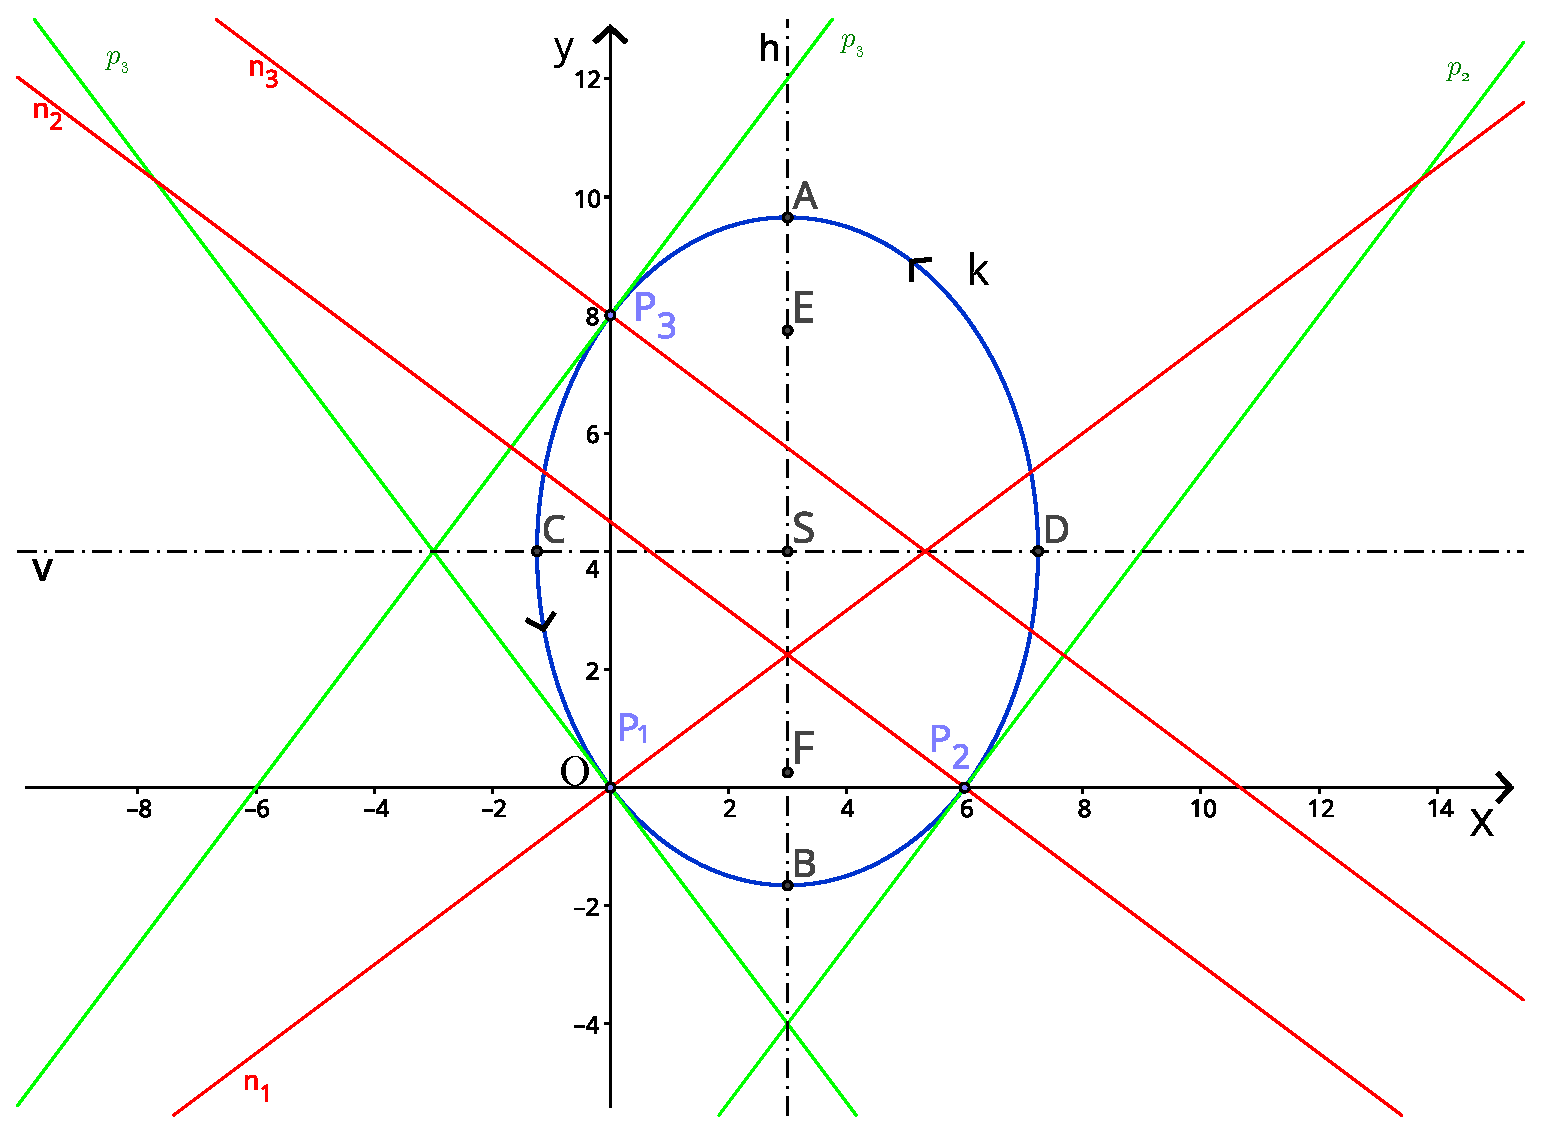
\includegraphics[width=0.9\textwidth]{elipsa2.eps}
			\caption{Elipsa pro $t \in \langle0, 2\pi\rangle$}
								
		\end{figure}
		\clearpage						
		\section{Hyperbola}
		Uvažujme hyperbolu o středu $O=[0,0]$, osy hyperboly jsou souřadnicové osy. Rovnice hyperboly ve středovém tvaru je
		$$\frac{x^2}{a^2}-\frac{y^2}{b^2}=1.$$
		hlavní osa je osa \textit{x}, vrcholy jsou body $A=[a, 0]$, $B[-a, 0]$ \\
		nebo
		$$-\frac{x^2}{b^2}+\frac{y^2}{a^2}=1.$$
		hlavní osa je osa \textit{y}, vrcholy jsou body $A=[0, a]$, $B[0, -a]$ \\[10pt]
			Kladné číslo \textit{a} je velikost hlavní poloosy, kladné číslo \textit{b} je velikost vedlejší poloosy.
			\begin{figure}[H]
				\centering
				\begin{subfigure}{0.5\textwidth}
					\centering
					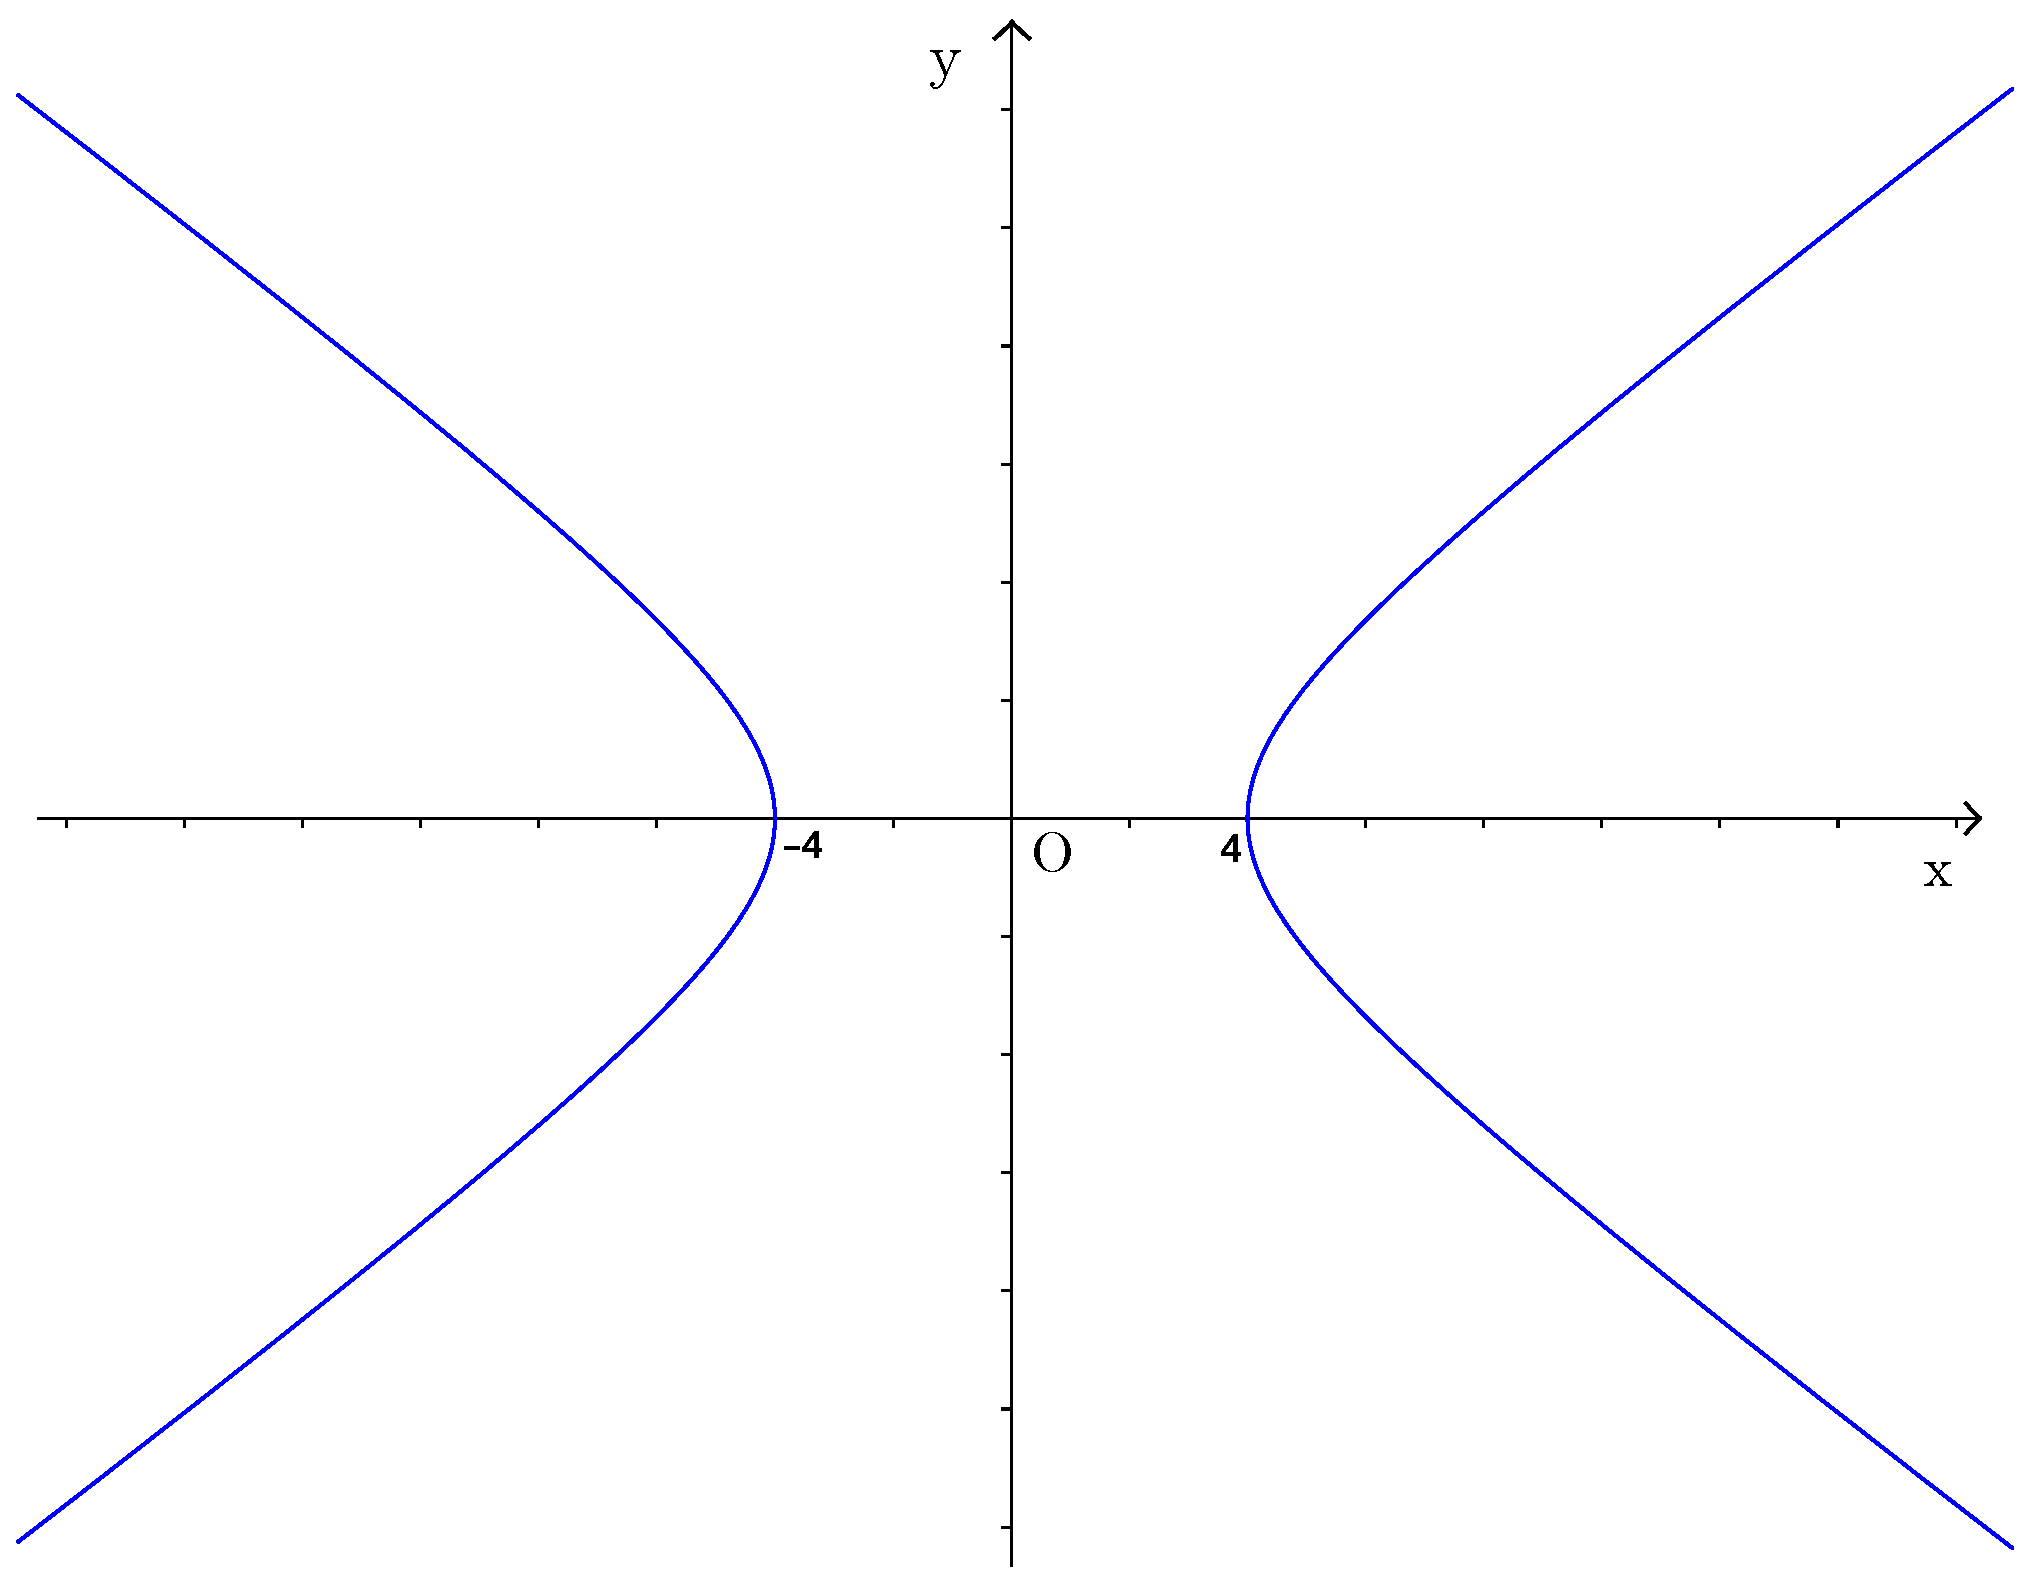
\includegraphics[width=\textwidth]{hyperbola-teorie1a.eps}
					\caption{Hyperbola $\frac{x^2}{16}-\frac{y^2}{9}=1$}
				\end{subfigure}%
				\begin{subfigure}{0.5\textwidth}
					\centering
					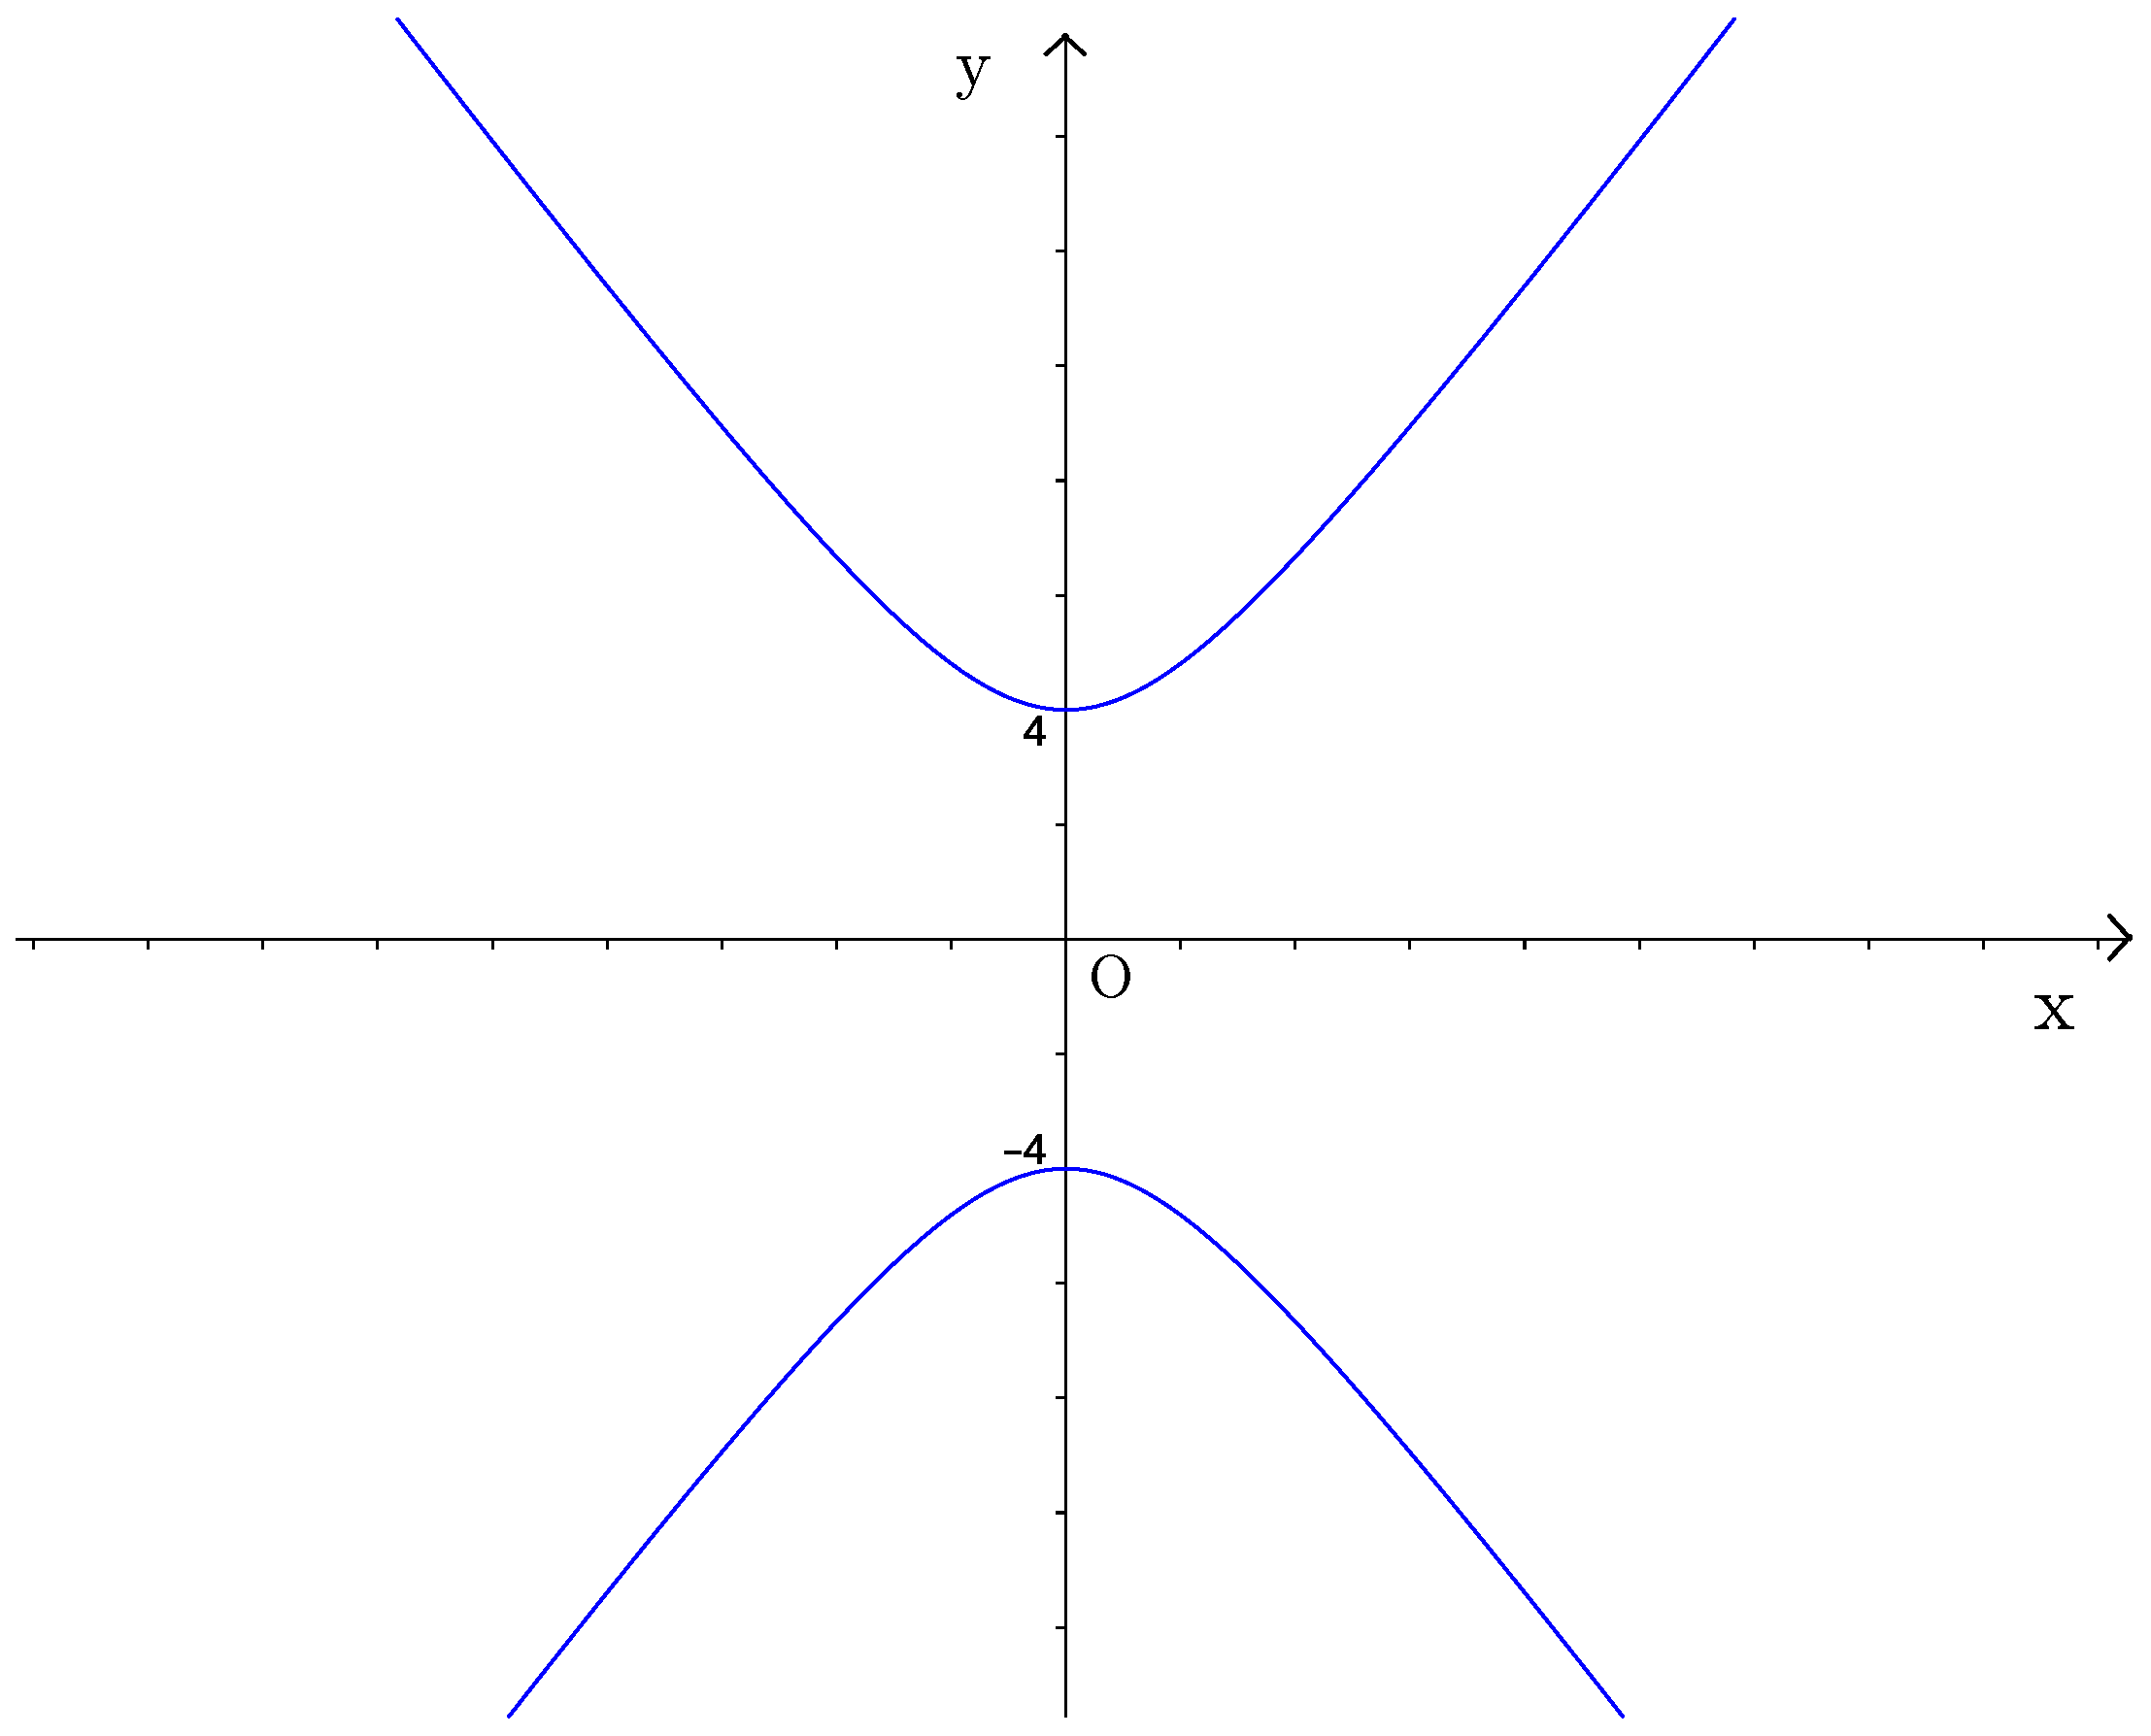
\includegraphics[width=\textwidth]{hyperbola-teorie1b.eps}
					\caption{Hyperbola $-\frac{x^2}{9}+\frac{y^2}{16}=1$}
				\end{subfigure}
				\caption{Hyperboly v základní poloze}
			\end{figure}
			Připomeňme, že může být $a>b$ i $a<b$. Je-li $a=b$, hyperbola se nazývá rovnoosá. Každá hyperbola má 2 tzv. \textit{asymptoty},
			jsou to přímky, ke kterým se tato křivka přibližuje. \\[10pt]
			Pro hyperbolu $\frac{x^2}{a^2}-\frac{y^2}{b^2}=1$ získáme asymptoty z rovnice $\frac{x^2}{a^2}-\frac{y^2}{b^2}=0$, tj.:
			$$\left(\frac{x}{a}-\frac{y}{b}\right)\cdot\left(\frac{x}{a}+\frac{y}{b}\right)=0.$$
			Rovnice asymptot ve směrnicovém tvaru jsou
			$$y=\frac{b}{a}x$$
			a
			$$y=-\frac{b}{a}x.$$
			Pro hyperbolu $-\frac{x^2}{b^2}+\frac{y^2}{a^2}=1$ získáme asymptoty z rovnice $-\frac{x^2}{b^2}+\frac{y^2}{a^2}=0$, tj.:
			$$\left(-\frac{x}{b}+\frac{y}{a}\right)\cdot\left(\frac{x}{b}+\frac{y}{a}\right)=0,$$
			$$y=\frac{a}{b}x$$
			a
			$$y=-\frac{a}{b}x.$$
			\begin{figure}[H]
				\centering
				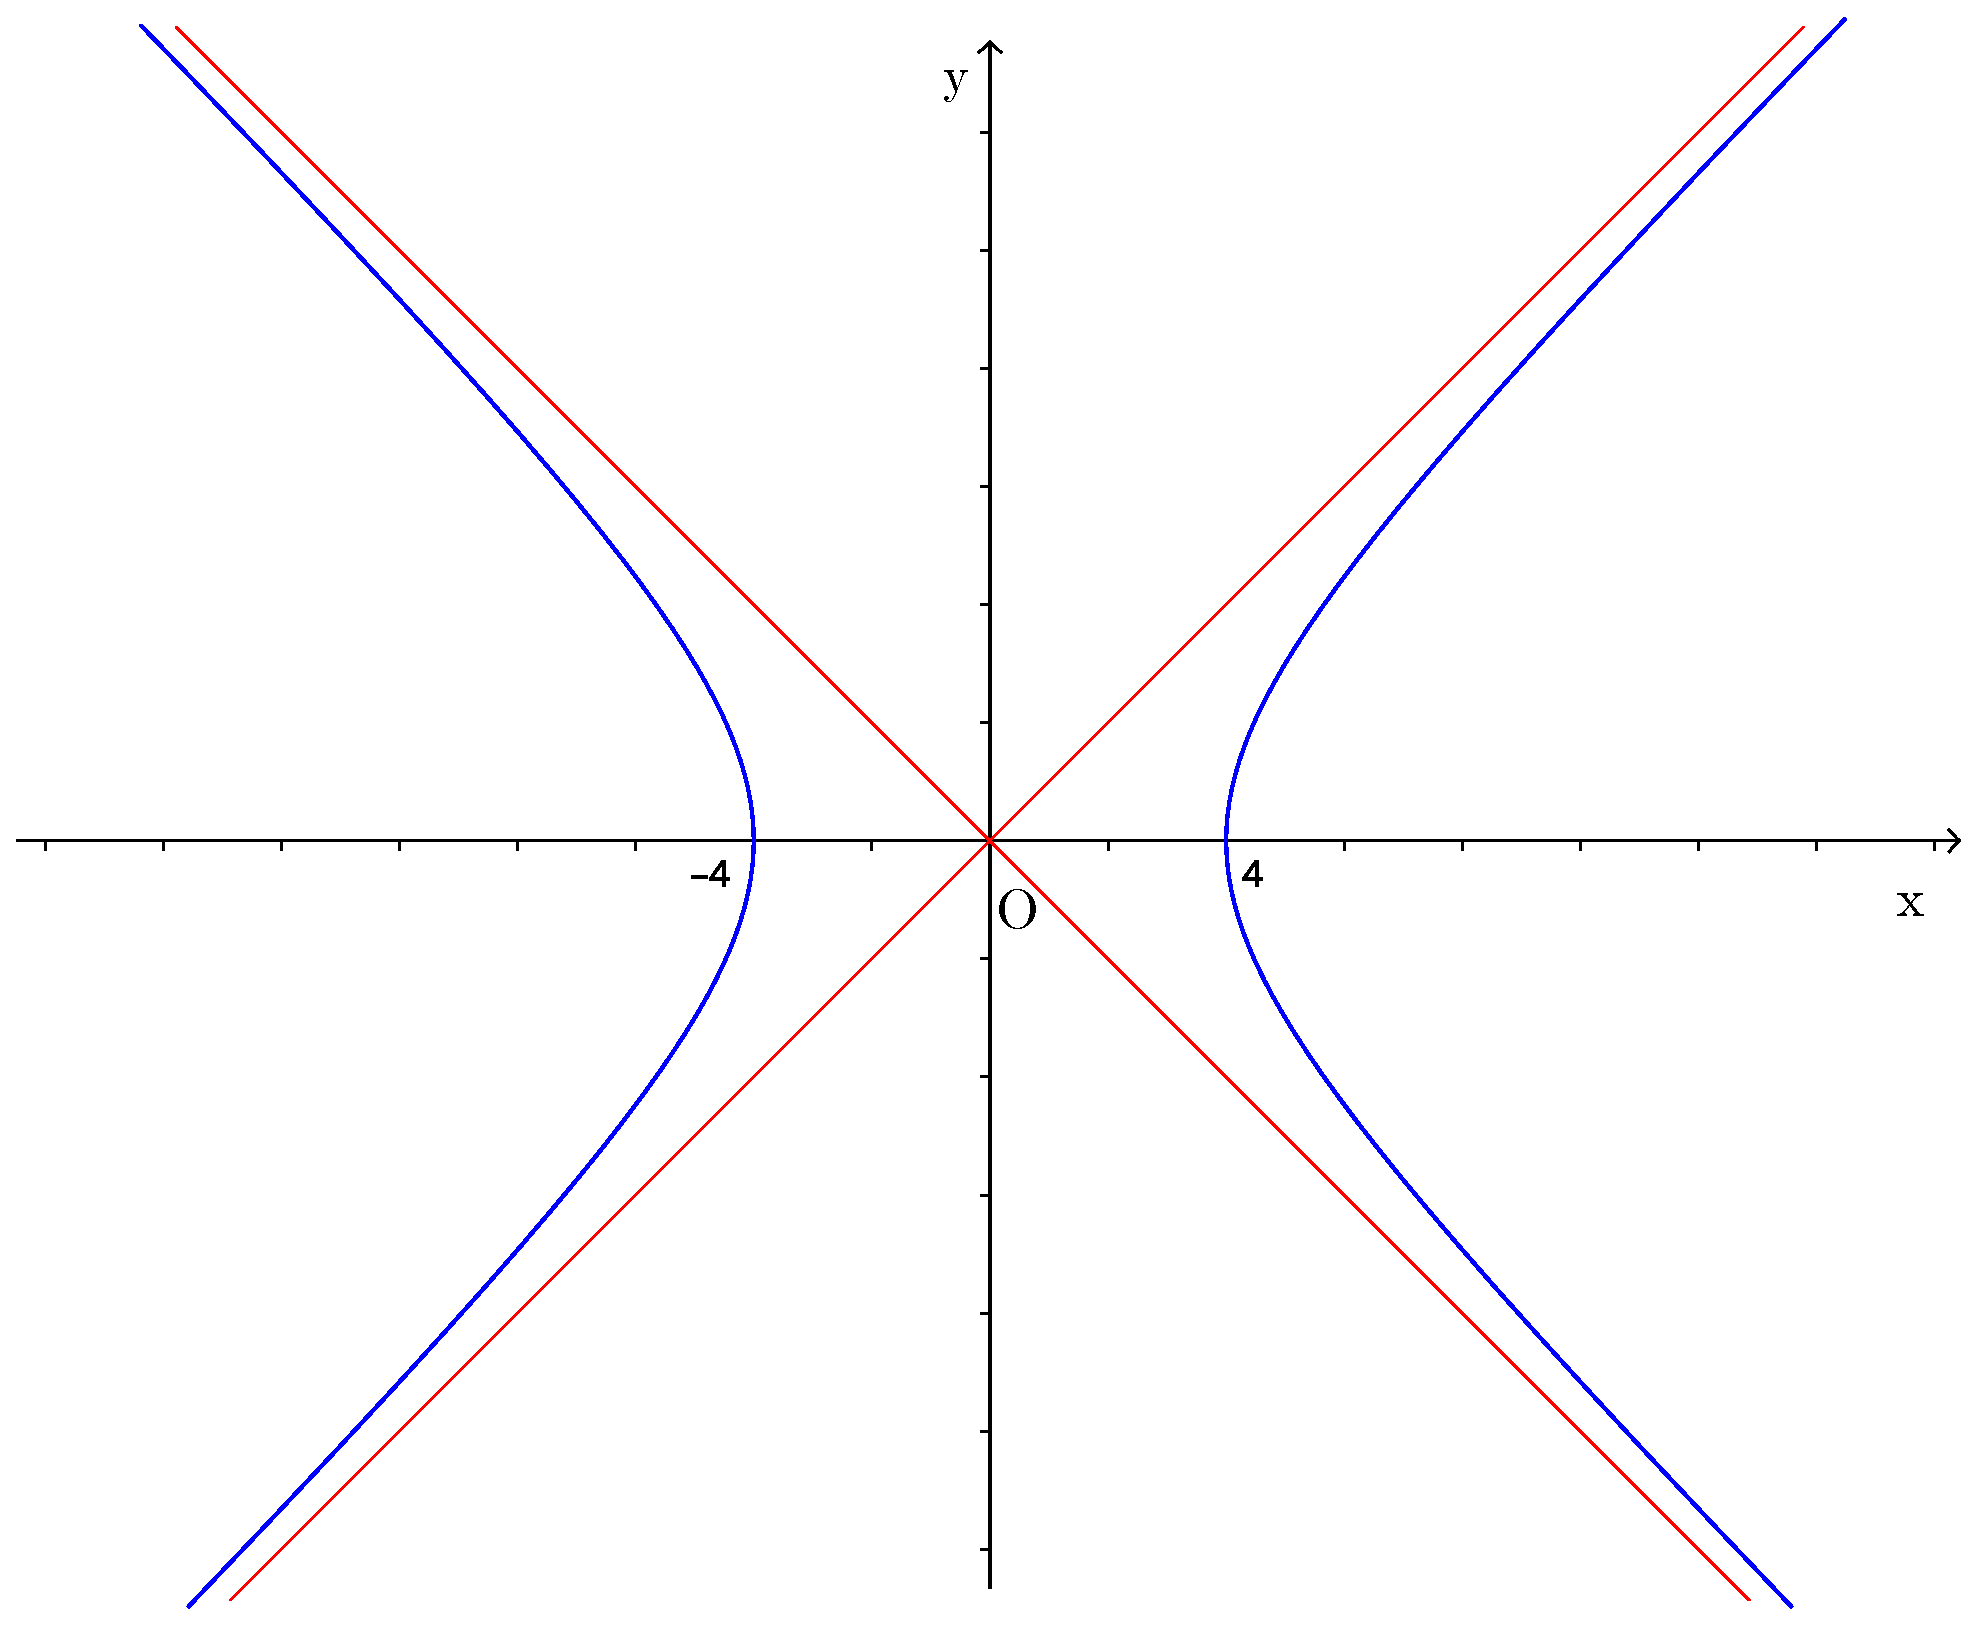
\includegraphics[width=0.75\textwidth]{hyperbola-teorie1c.eps}
				\caption{Asymptoty $y=x$ a $y=-x$ rovnoosé hyperboly $\frac{x^2}{16}-\frac{y^2}{16}=1$}					
			\end{figure}
			Vzhledem k předchozím poznatkům bychom pro parametrizaci hyperboly chtěli najít dvě funkce \textit{f} a \textit{g}, pro které
			by platilo $f^2(t)-g^2(t)=1$. \\[10pt]
			Takové funkce se nazývají hyperbolické a jsou jimi funkce
			$$f(t)=\frac{e^t+e^{-t}}{2}$$
			a
			$$g(t)=\frac{e^t-e^{-t}}{2}.$$
			$D_f=D_g=\mathbb{R}$
			\begin{figure}[H]
				\centering
				\begin{subfigure}{0.5\textwidth}
					\centering
					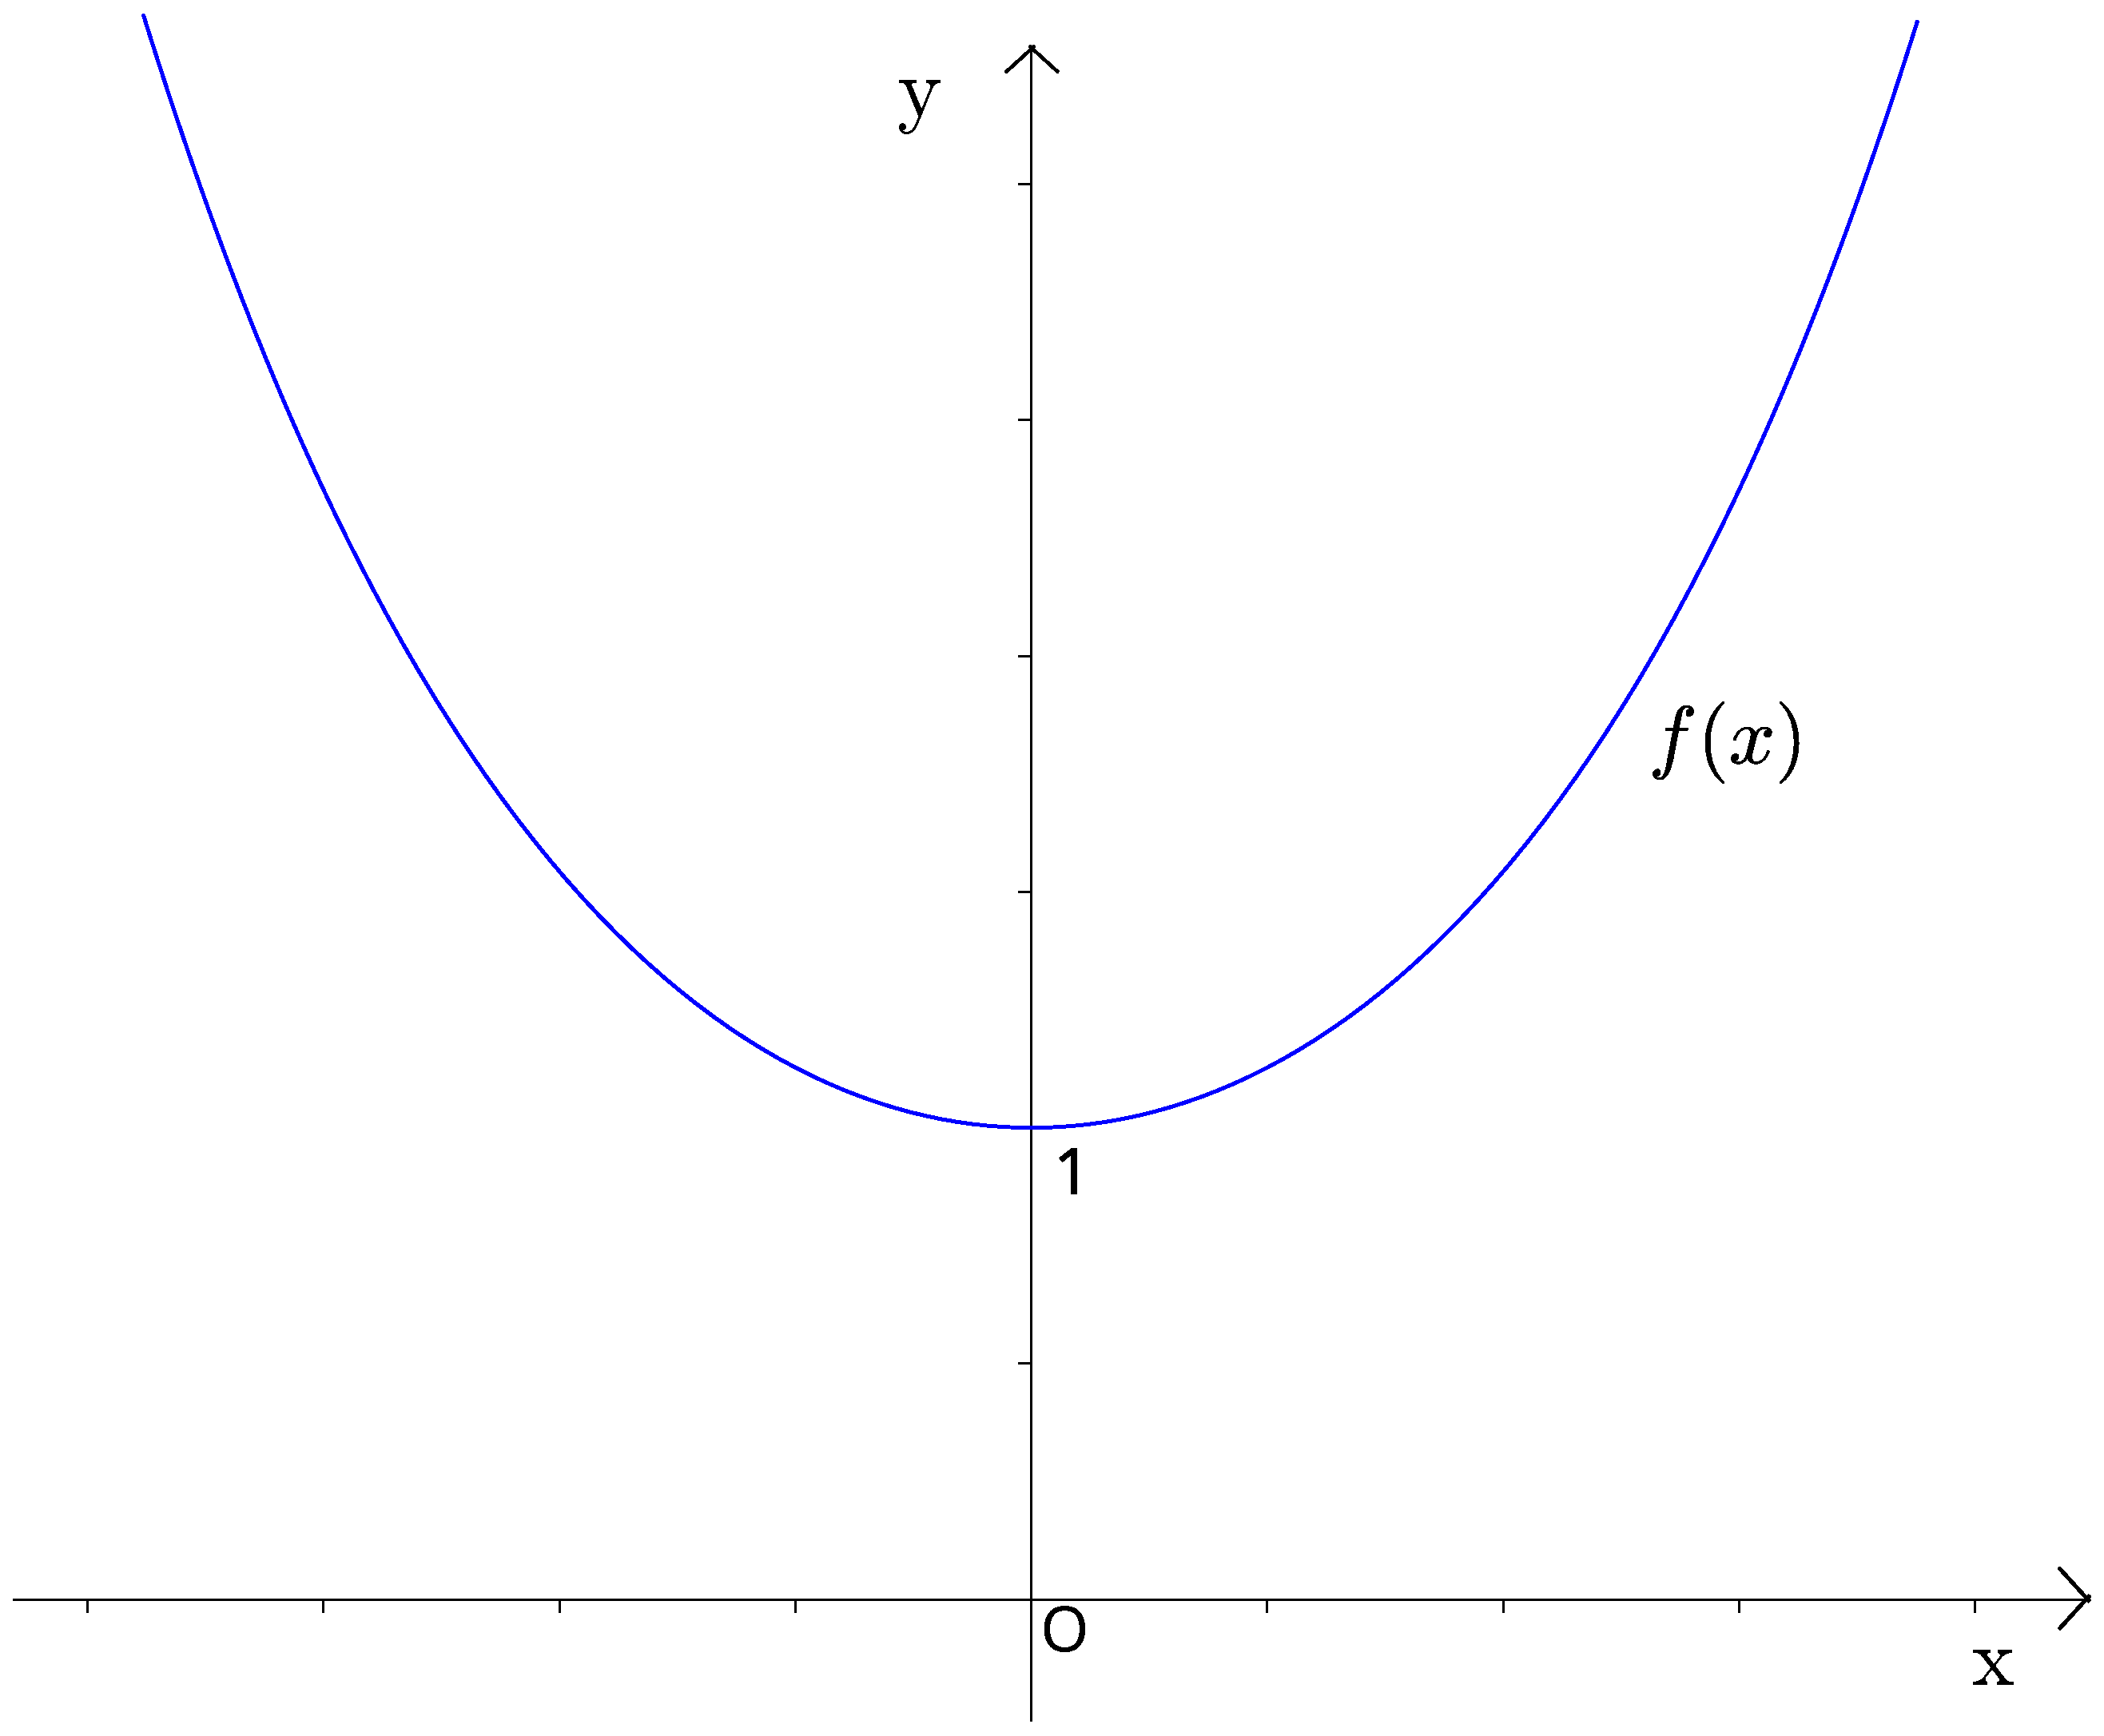
\includegraphics[width=\textwidth]{hyperbola-teorie2.eps}
					\caption{Funkce \textit{f}}
				\end{subfigure}%
				\begin{subfigure}{0.5\textwidth}
					\centering
					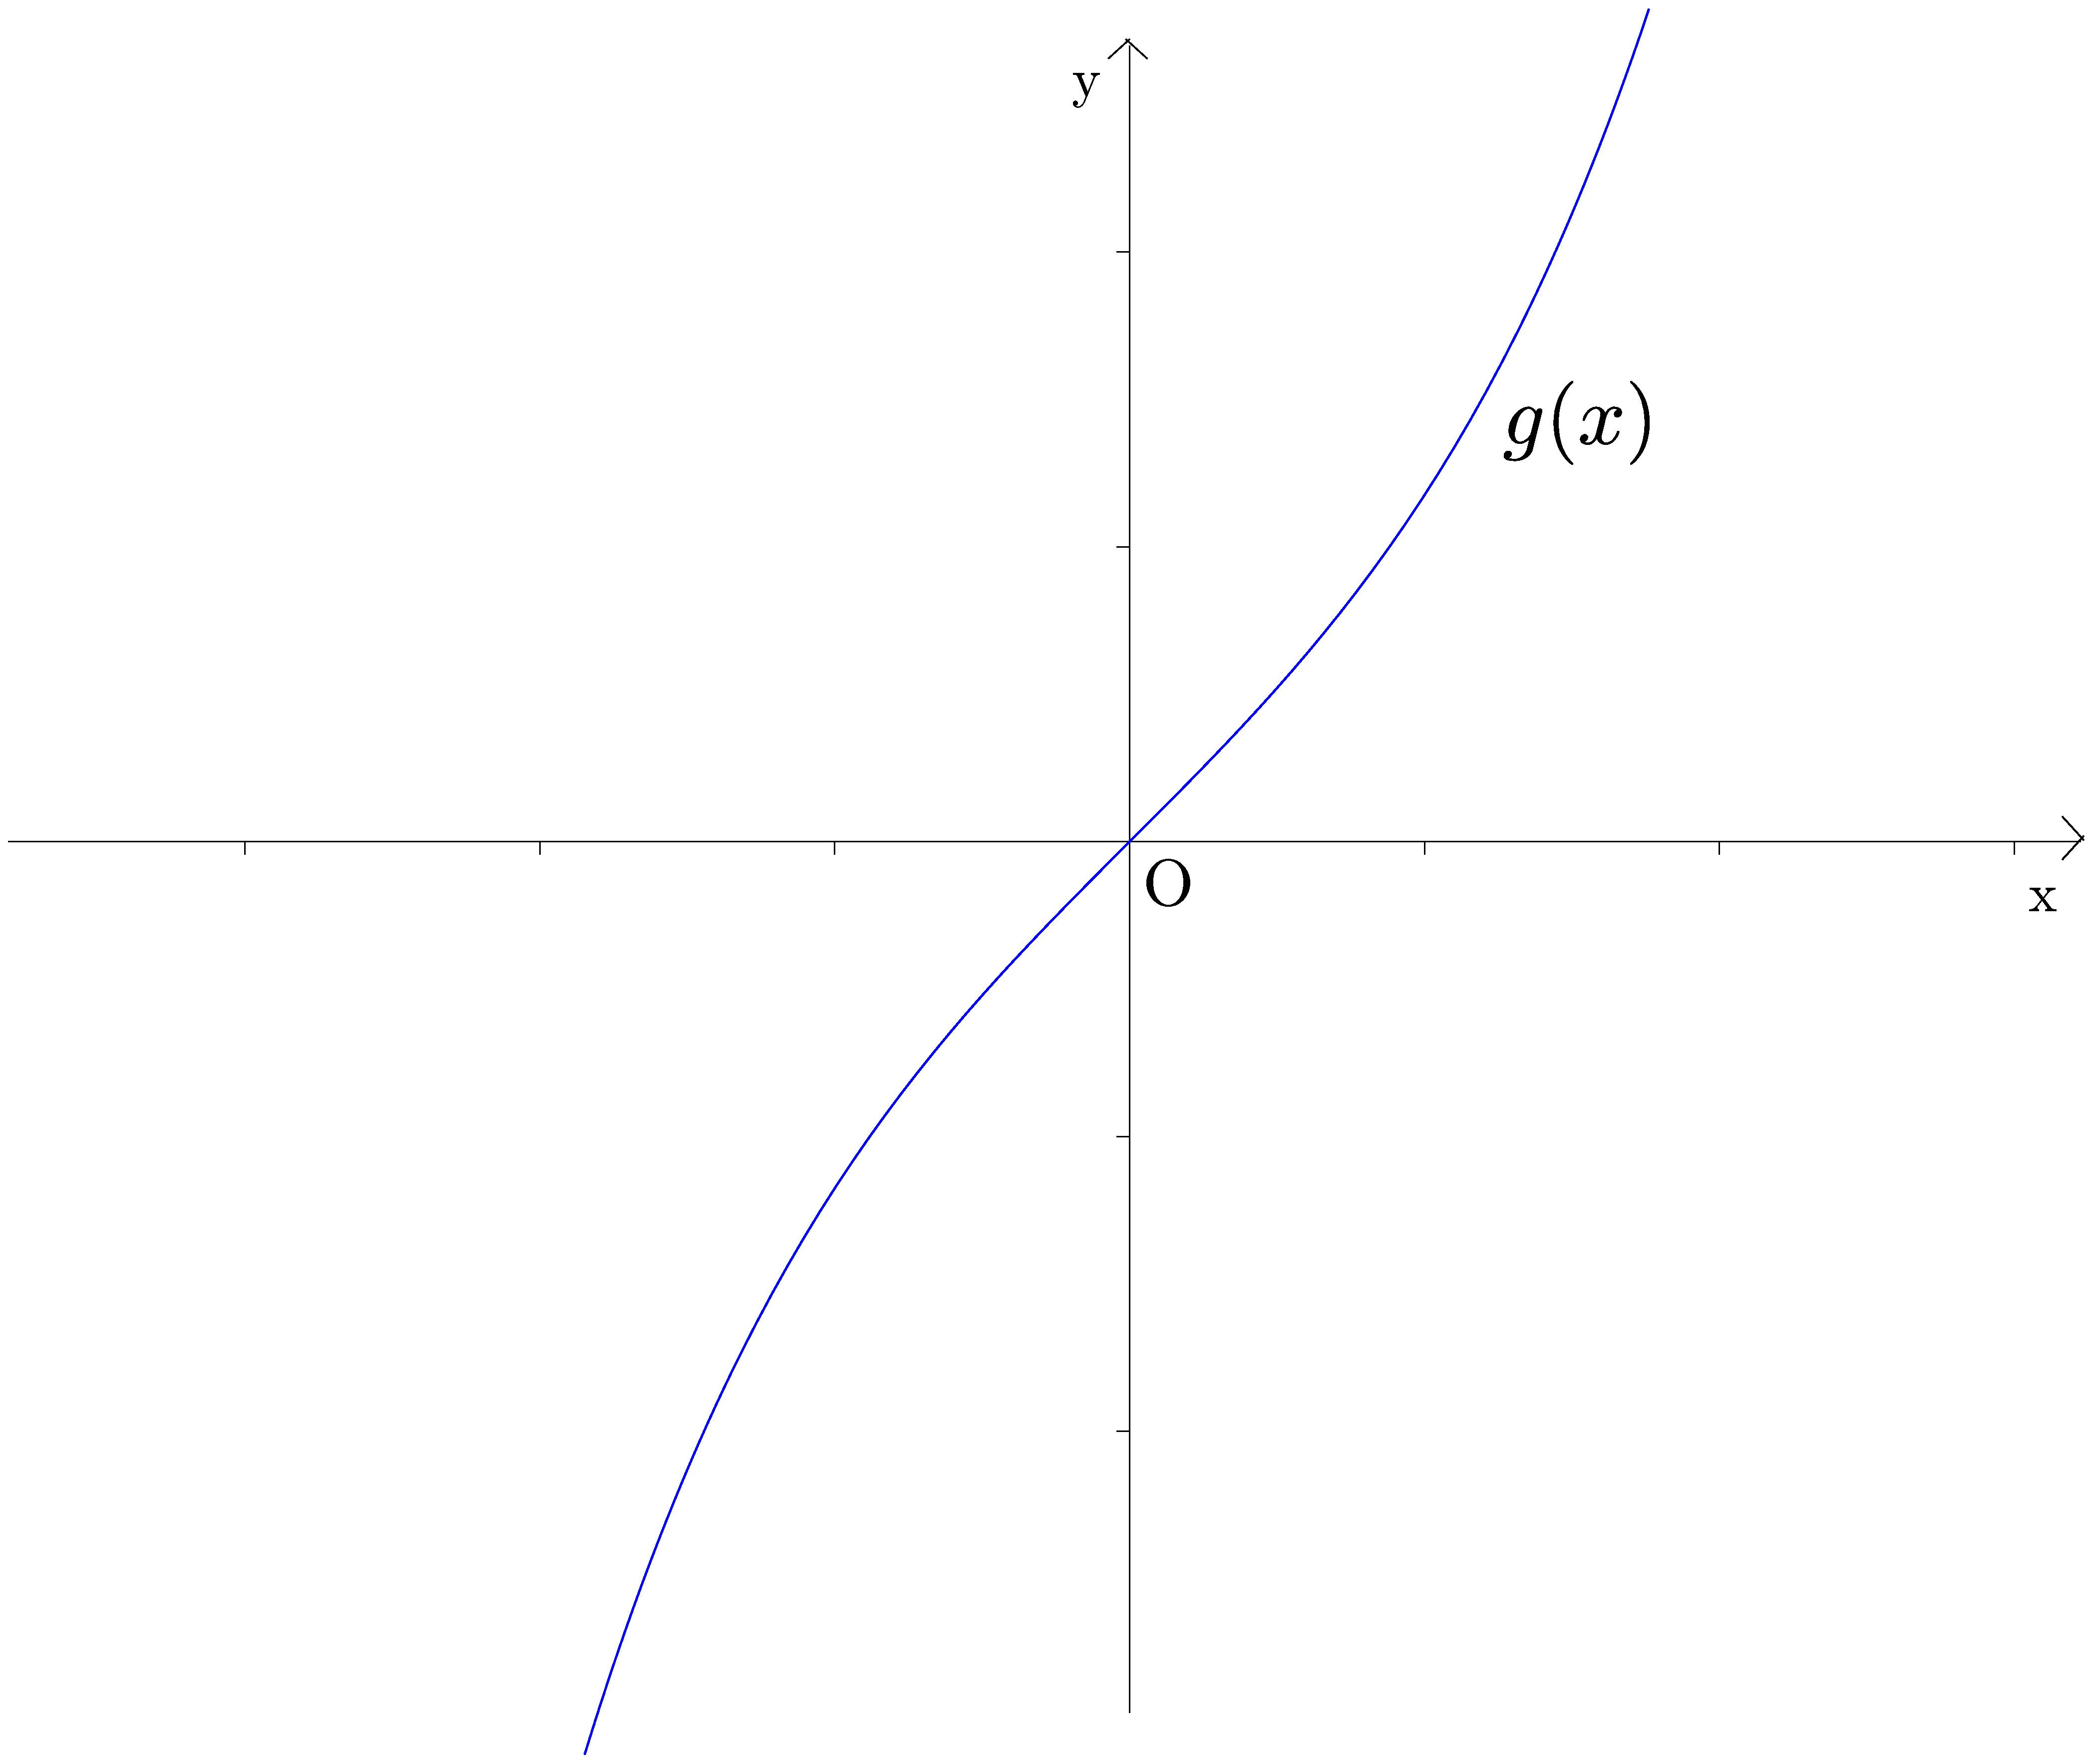
\includegraphics[width=\textwidth]{hyperbola-teorie3.eps}
					\caption{Funkce \textit{g}}
				\end{subfigure}
				\caption{Grafy hyperbolických funkcí \textit{f} a \textit{g}}
			\end{figure}
			\noindent Snadno ukážeme, že $f'(t)=g(t)$, $f''(t)=f(t)$, $g'(t)=f(t)$ a $f''(t)=g(t)$. \\[10pt]
			Něco podobného známe pro funkce  $\sin$ a $\cos$ (až na znaménka): $(cos{t})'=-\sin{t}$,\\ $(cos{t})''=-\cos{t}$
			, $(\sin{t})'=\cos{t}$ a $(sin{t})''=-\sin{t}$. \\[10pt]
			Proto se funkce $f(t)=\frac{e^t+e^{-t}}{2}$ nazývá  kosinus hyperbolický, značíme $\cosh{t}$. Funkce \\ $g(t)=\frac{e^t-e^{-t}}{2}$
			se nazývá sinus hyperbolický a značíme $\sinh{t}$. \\[10pt]
			Nyní si ověříme, že platí $\cosh^2{t}-\sinh^2{t}=1$:
			\begin{align*}
				\left(\frac{1}{2}(e^t+e^{-t})\right)^2                                             & - \left(\frac{1}{2}(e^t-e^{-t})\right)^2                                             \\
				\frac{1}{4} \left(e^{2t} + 2 e^t \cdot e^{-t} + e^{-2t}\right)                     & - \frac{1}{4} \left(e^{2t} - 2 e^t \cdot e^{-t} + e^{-2t}\right)                     \\
				\cancel{\frac{1}{4}e^{2t}}+\frac{1}{4} \cdot 2\cdot1 + \cancel{\frac{1}{4}e^{-2t}} & - \cancel{\frac{1}{4}e^{2t}}+\frac{1}{4} \cdot 2 \cdot 1-\cancel{\frac{1}{4}e^{-2t}} \\
				\frac{1}{2}+\frac{1}{2}                                                            & = 1                                                                                  
			\end{align*}
			\clearpage
			\noindent Pro parametrizaci hyperboly
			$$\frac{x^2}{a^2}-\frac{y^2}{b^2}=1$$
			dáme do rovnosti $\frac{x}{a}=\cosh{t}$ a $\frac{y}{b}=\sinh{t}$ a získáme parametrické vyjádření
			$$k(t)=\left[a\cosh{t}, b\sinh{t}\right], t \in \mathbb{R}.$$
			Toto je ovšem parametrický popis jedné větve hyperboly. \\
			Víme, že  $\cosh{t} \geq 1$ pro všechna $t \in \mathbb{R}$ (viz graf \textit{f}). Uvedený parametrický popis je popisem pravé větve hyperboly. Parametrický popis obou větví (symetrie podle osy \textit{y}) je
			$$k(t)=\left[\pm a\cosh{t}, b\sinh{t}\right], t \in \mathbb{R}.$$
			Pro parametrický popis hyperboly  $-\frac{x^2}{b^2}+\frac{y^2}{a^2}=1$ dáme do rovnosti $\frac{x}{b}=\sinh{t}$ a $\frac{y}{a}=\cosh{t}$ (zdůrazněme, že se rozhodujeme podle znamének v obecné rovnici). \\
			Parametrický popis obou větví je
			$$k(t)=\left[b\sinh{t}, \pm a\cosh{t} \right], t \in \mathbb{R}.$$
			(znaménko \textit{+} je pro horní větev, znaménko \textit{-} je pro dolní větev).
			Souřadnice vrcholů jsou $k(0)=[b\sinh{0}, \pm a\cosh{0}] = [0, \pm a \cdot 1] = [0, \pm a]$. \\
			Pro obecnější případ, kdy střed hyperboly je bod $S=[m, n]$ a rovnice ve středovém tvaru je
			$$\frac{(x-m)^2}{a^2}-\frac{(y-n)^2}{b^2}=1$$
			nebo
			$$-\frac{(x-m)^2}{b^2}+\frac{(y-n)^2}{a^2}=1$$
			změníme předchozí parametrizaci přičtením vektoru posunutí $S-O=(m, n)$. \\
			Parametrický popis hyperboly $\frac{(x-m)^2}{a^2}-\frac{(y-n)^2}{b^2}=1$ je
			$$k(t)=[m \pm a\cosh{t}, n+b\sinh{t}], t \in \mathbb{R}.$$
			parametrický popis hyperboly $-\frac{(x-m)^2}{b^2}+\frac{(y-n)^2}{a^2}=1$ je
			$$k(t)=[m+b\sinh{t}, n \pm a\cosh{t}], t \in \mathbb{R}.$$
			Při kreslení hyperboly s využitím grafického programu musíme interval pro parametr \textit{t} omezit z obou stran, např. $t \in \langle-10, 10 \rangle$
			\clearpage
			\subsection*{Příklad 1}
			Napište parametrické vyjádření hyperboly zadané obecnou rovnicí
			$$9x^2-16y^2-54x+128y-319=0.$$
			Napište souřadnice vrcholů a ohnisek hyperboly. Dále napište obecné rovnice asymptot. \\[10pt]
			\textbf{Řešení:} Obecnou rovnici upravíme na středový tvar:
			$$\frac{(x-3)^2}{16}-\frac{(y-4)^2}{9}=1.$$
			Střed hyperboly je bod $S=[3,4]$, hlavní osa je rovnoběžná s osou \textit{x}. Velikost hlavní poloosy
			je $a=4$, velikost vedlejší poloosy je $b=3$. \\
			Pro parametrizaci dáme do rovnosti \\
			\begin{align*}
				\frac{x-3}{4} & =\cosh{t}, \\ \frac{y-4}{3}&=\sinh{t}
			\end{align*}
			a získáme parametrický popis pravé větve
			$$k(t)=[3+4\cosh{t}, 4+3\sinh{t}], t \in \mathbb{R}\text{.}$$
			Parametrický popis obou větví je
			$$k(t)=[3\pm4\cosh{t}, 4+3\sinh{t}], t \in \mathbb{R}\text{.}$$
			Vrcholy můžeme vypočítat z parametrického vyjádření
			\begin{align*}
				k(0)=[3\pm4\cdot1, 4+3\cdot0] \text{,} \\
				\text{tedy }                           
				A=[7, 4], B=[-1, 4].                   
			\end{align*}
			Pro velikost excentricity \textit{e} platí vztah $e^2=a^2+b^2$. V našem případě \\ $e^2=16+9$
			a tedy $e=5$.
			\begin{align*}
				E & =[3+5, 4]=[8, 4] \\
				F & =[3-5, 4]=[-2,4] 
			\end{align*}
			Rovnice asymptot získáme z rovnice
			\begin{align*}
				\frac{(x-3)^2}{16}    & -\frac{(y-4)^2}{9}=0      \\
				\text{tj.: } 9(x-3)^2 & -16(y-4)^2=0              \\
				[3(x-3)]^2            & -[4(y-4)]^2=0             \\
				[3(x-3)-4(y-4)]       & \cdot[3(x-3)+4(y-4)] = 0. 
			\end{align*}
			Rovnice asymptot jsou
			\begin{align*}
				a_1: 3x-4y+7  & =0  \\
				\text{a}\\
				a_2: 3x+4y-25 & =0. 
			\end{align*}
			\begin{figure}[H]
				\centering
				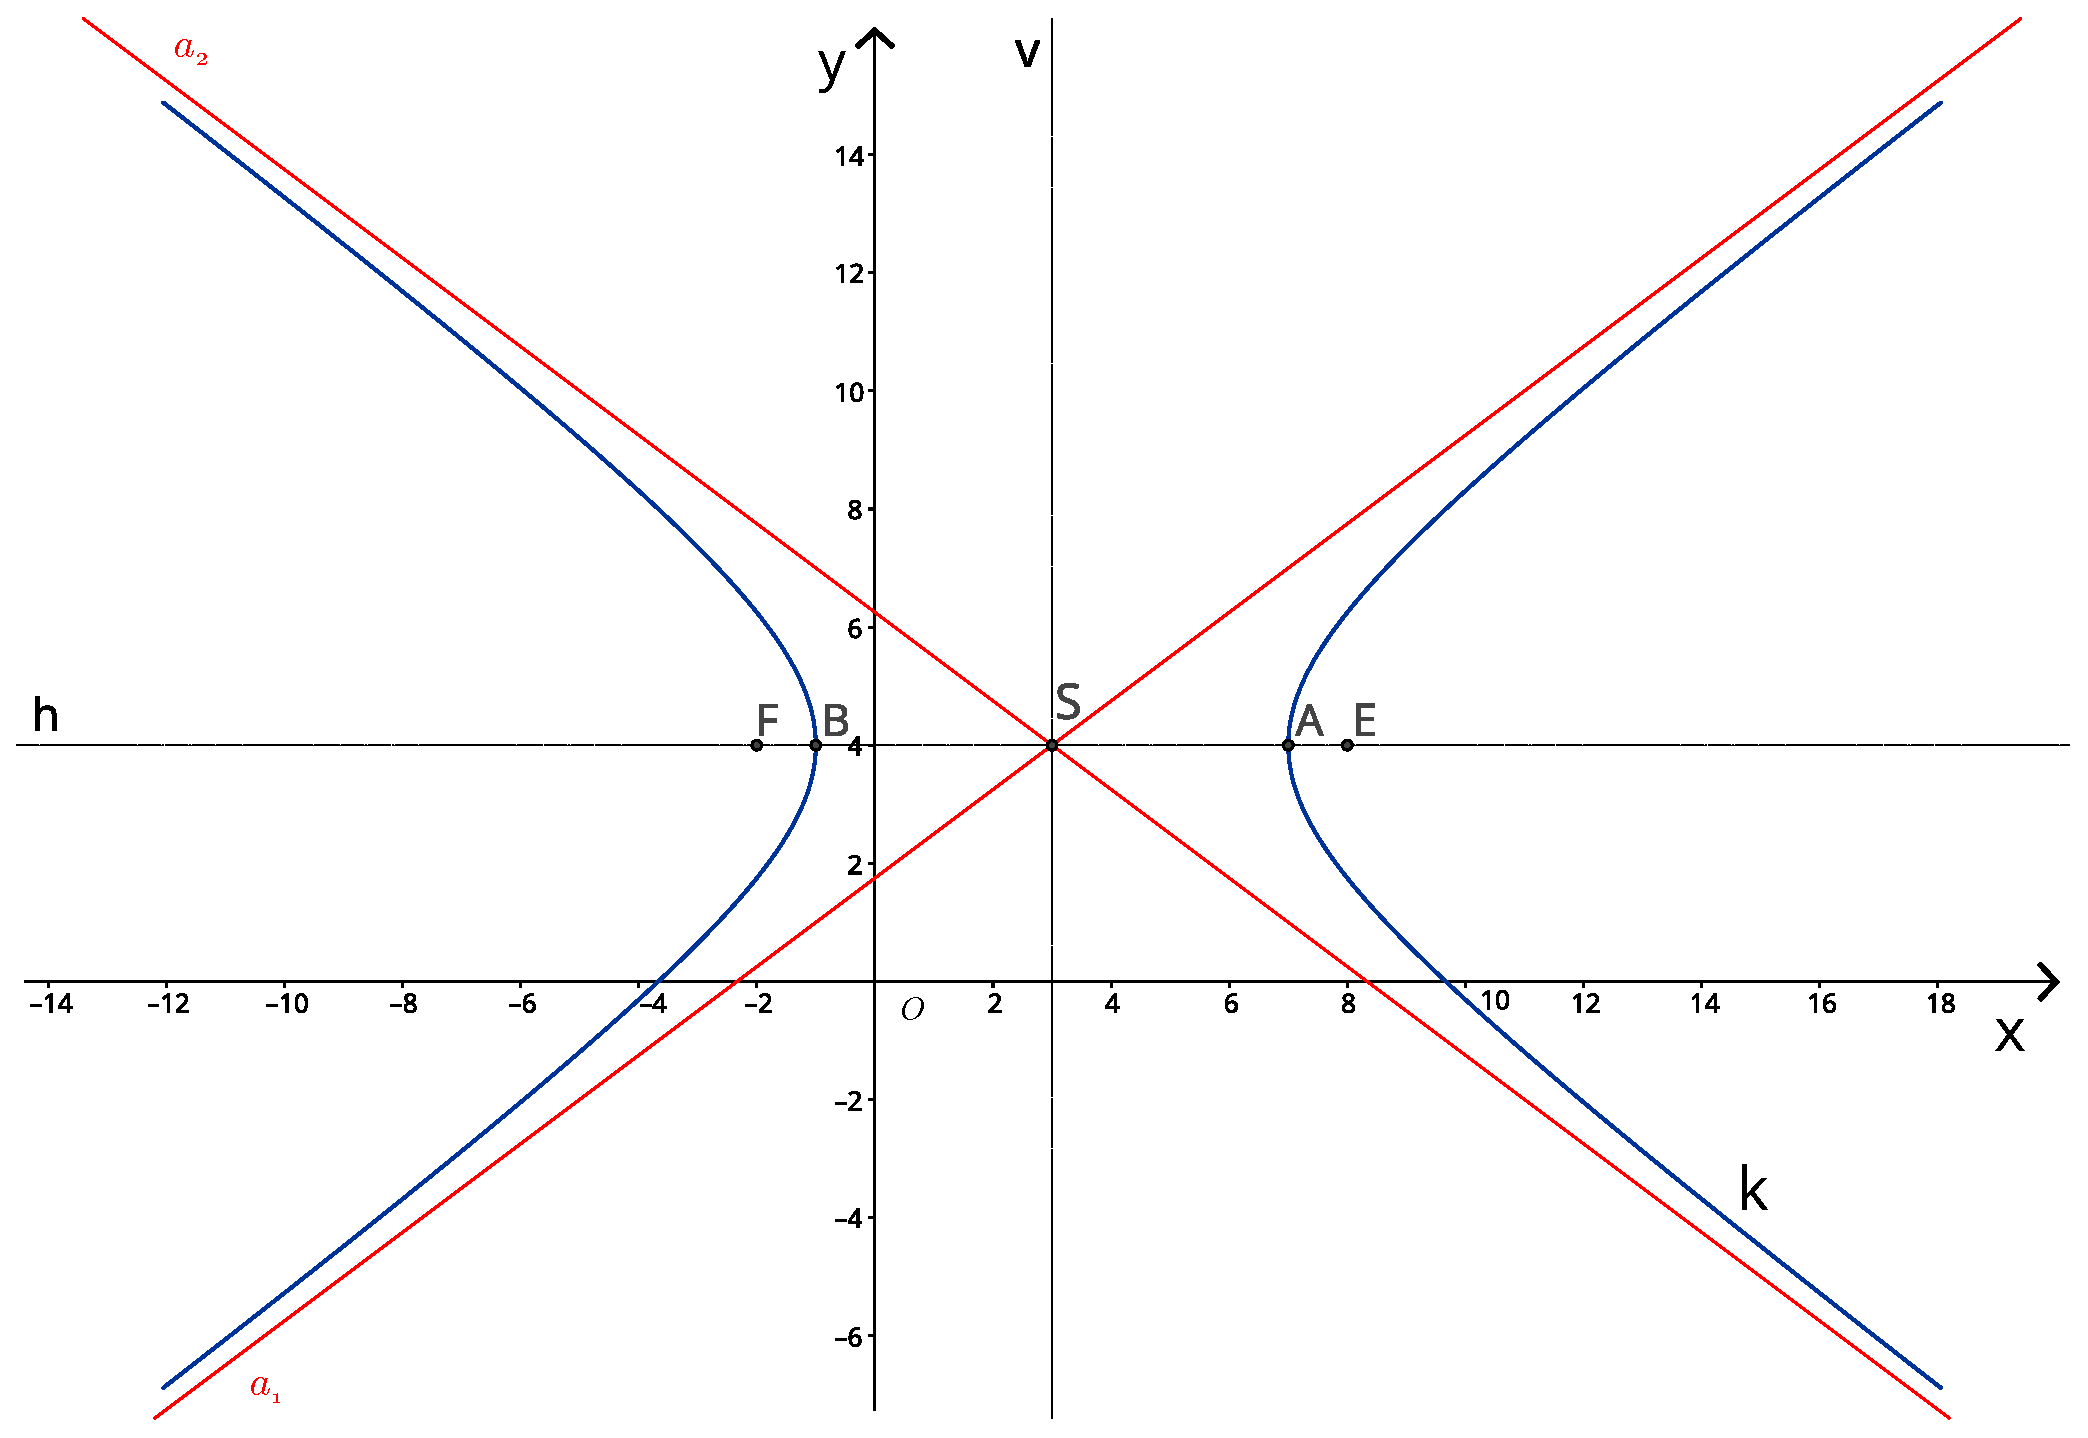
\includegraphics[width=\textwidth]{hyperbola1.eps}
				\caption{Hyperbola pro $t \in \langle-2, 2\rangle$}
									
			\end{figure}
			\clearpage
			\subsection*{Příklad 2}
			Napište parametrické vyjádření hyperboly zadané obecnou rovnicí
			$$9x^2-16y^2-54x+128y-31=0.$$
			Napište souřadnice vrcholů, ohnisek a průsečíků hyperboly se souřadnicovými osami. Dále napište obecné rovnice asymptot.\\[5pt]
			\textbf{Řešení:} Obdobně jako v minulém příkladu upravíme obecnou rovnici na středový tvar:
			$$\frac{(y-4)^2}{9}-\frac{(x-3)^2}{16}=1.$$
			Střed hyperboly je bod $S=[3,4]$, hlavní osa je rovnoběžná s osou \textit{y}. Velikosti poloos jsou $a=3$ a $b=4$. \\
			Pro parametrizaci dáme do rovnosti \\
			\begin{align*}
				\frac{y-4}{3} & =\cosh{t}, \\ \frac{x-3}{4}&=\sinh{t}
			\end{align*}
			a získáme parametrický popis horní větve
			$$k(t)=[3+4\sinh{t}, 4+3\cosh{t}], t \in \mathbb{R}\text{.}$$
			Parametrický popis obou větví je
			$$k(t)=[3+4\sinh{t}, 4\pm3\cosh{t}], t \in \mathbb{R}\text{.}$$
			Vrcholy můžeme vypočítat z parametrického vyjádření
			\begin{align*}
				k(0)=[3+4\cdot0, 4\pm3\cdot1] \text{,} \\
				\text{tedy }                           
				A=[3, 7], B=[3, 1].                    
			\end{align*}
			Pro velikost excentricity \textit{e} platí vztah $e^2=a^2+b^2$. V našem případě \\ $e^2=9+16$
			a tedy $e=5$.
			\begin{align*}
				E & =[3, 4+5]=[3, 9] \\
				F & =[3, 4-5]=[3,-1] 
			\end{align*}
			Rovnice asymptot získáme z rovnice
			\begin{align*}
				\frac{(y-4)^2}{9}-\frac{(x-3)^2}{16}=0 \\
				\text{tj.: } 16(y-4)^2-9(x-3)^2 & =0                        \\
				[4(y-4)]^2-[3(x-3)]^2           & =0                        \\
				[4(y-4)-3(x-3)]                 & \cdot[4(y-4)+3(x-3)] = 0. 
			\end{align*}
			Rovnice asymptot jsou
			\begin{align*}
				a_1 & : 3x-4y+7  =0  \\
				\text{a}\\
				a_2 & : 3x+4y-25 =0. 
			\end{align*}
			Souřadnice průsečíků hyperboly se souřadnicovými osami můžeme určit a) z obecné rovnice nebo b) z rovnice ve středovém tvaru
			nebo c) z parametrického vyjádření.
			\begin{enumerate}
				\item Průsečíky s osou \textit{x} ($y=0$) \\
				      \small
				      \begin{minipage}[t]{0.5\textwidth}
				      	a)
				      	\begin{align*}
				      		9x^2    & -54x-31=0                     \\
				      		x_{1,2} & = \frac{54\pm\sqrt{4032}}{18} \\
				      		x_{1,2} & = \frac{54\pm24\sqrt{7}}{18}  \\
				      		x_1     & = 3 + \frac{4\sqrt{7}}{3}     \\
				      		x_2     & = 3 - \frac{4\sqrt{7}}{3}     
				      	\end{align*}
				      \end{minipage}
				      \begin{minipage}[t]{0.5\textwidth}
				      	b)
				      	\begin{align*}
				      		\frac{16}{9}-\frac{(x-3)^2}{16} & = 1                       \\
				      		-\frac{(x-3)^2}{16}             & = -\frac{7}{9}            \\
				      		(x-3)^2                         & = \frac{7}{9}\cdot16      \\
				      		|x-3|                           & = \frac{4\sqrt{7}}{3}     \\
				      		x_1                             & = 3 + \frac{4\sqrt{7}}{3} \\
				      		x_2                             & = 3 - \frac{4\sqrt{7}}{3} 
				      	\end{align*}
				      \end{minipage}
				      c) průsečíky s osou \textit{x} má pouze dolní větev
				      				      
				      \begin{minipage}[t]{0.5\textwidth}
				      	\begin{align*}
				      		4-3\cosh{t}=0                       \\
				      		4-3\cdot\frac{1}{2}(e^t+e^{-t}) = 0 \\
				      		8-3\cdot(e^t+e^{-t}) = 0            \\
				      		8-3e^t-3\frac{1}{e^t} = 0           \\
				      		8e^t-3(e^t)^2-3 = 0                 \\
				      		3(e^t)^2-8e^t+3 = 0                 \\
				      		e^t = \frac{8\pm\sqrt{28}}{6}       \\
				      		e^t = \frac{4\pm\sqrt{7}}{3}        
				      	\end{align*}
				      \end{minipage}				    
				      \begin{minipage}[t]{0.5\textwidth}
				      	\vspace{10pt}
				      	pro $e^t=\frac{4+\sqrt{7}}{3}$ je $\sinh{t} = \frac{1}{2}(e^t-\frac{1}{e^t})=$
				      	\begin{align*}
				      		  & = \frac{1}{2}(\frac{4+\sqrt{7}}{3}-\frac{3}{4+\sqrt{7}}) =    \\
				      		  & = \frac{1}{2}(\frac{4+\sqrt{7}}{3}-\frac{3(4-\sqrt{7})}{9}) = \\
				      		  & = \frac{1}{2}\cdot\frac{2\sqrt{7}}{3} = \frac{\sqrt{7}}{3}    
				      	\end{align*}
				      	pro $e^t=\frac{4-\sqrt{7}}{3}$ je $\sinh{t} = \frac{1}{2}(\frac{4-\sqrt{7}}{3}-\frac{3}{4-\sqrt{7}}) = -\frac{\sqrt{7}}{3}$
				      	\begin{align*}
				      		x_1 & = 3 + \frac{4\sqrt{7}}{3} \\
				      		x_2 & = 3 - \frac{4\sqrt{7}}{3} 
				      	\end{align*}
				      \end{minipage}
				      \vspace{10pt}
				      Z výpočtu je vidět, že nejrychlejší výpočet vychází z rovnice ve středovém tvaru. Průsečíky s osou \textit{x} jsou body
				      $P_1=\left[3 + \frac{4\sqrt{7}}{3}, 0\right]$ a $P_2=\left[3-\frac{4\sqrt{7}}{3}, 0\right]$.
				      \normalsize
				\item Průsečíky s osou \textit{y} ($x=0$) vypočítáme z rovnice ve středovém tvaru:
				      \begin{align*}
				      	\frac{(y-4)^2}{9}-\frac{9}{16} & = 1                               \\
				      	\frac{(y-4)^2}{9}              & = 1+\frac{9}{16}                  \\
				      	(y-4)^2                        & = \frac{25}{16}\cdot 9            \\
				      	|y-4|                          & = \frac{5\cdot3}{4}               \\
				      	y_1                            & = 4 + \frac{15}{4} = \frac{31}{4} \\
				      	y_2                            & = 4 - \frac{15}{4} = \frac{1}{4}  
				      \end{align*}
				      Průsečíky s osou \textit{y} jsou body $P_4=\left[0, \frac{31}{4}\right]$ a $P_3=\left[0, \frac{1}{4}\right]$.
			\end{enumerate}
			\vfill
			\begin{figure}[H]
				\centering
				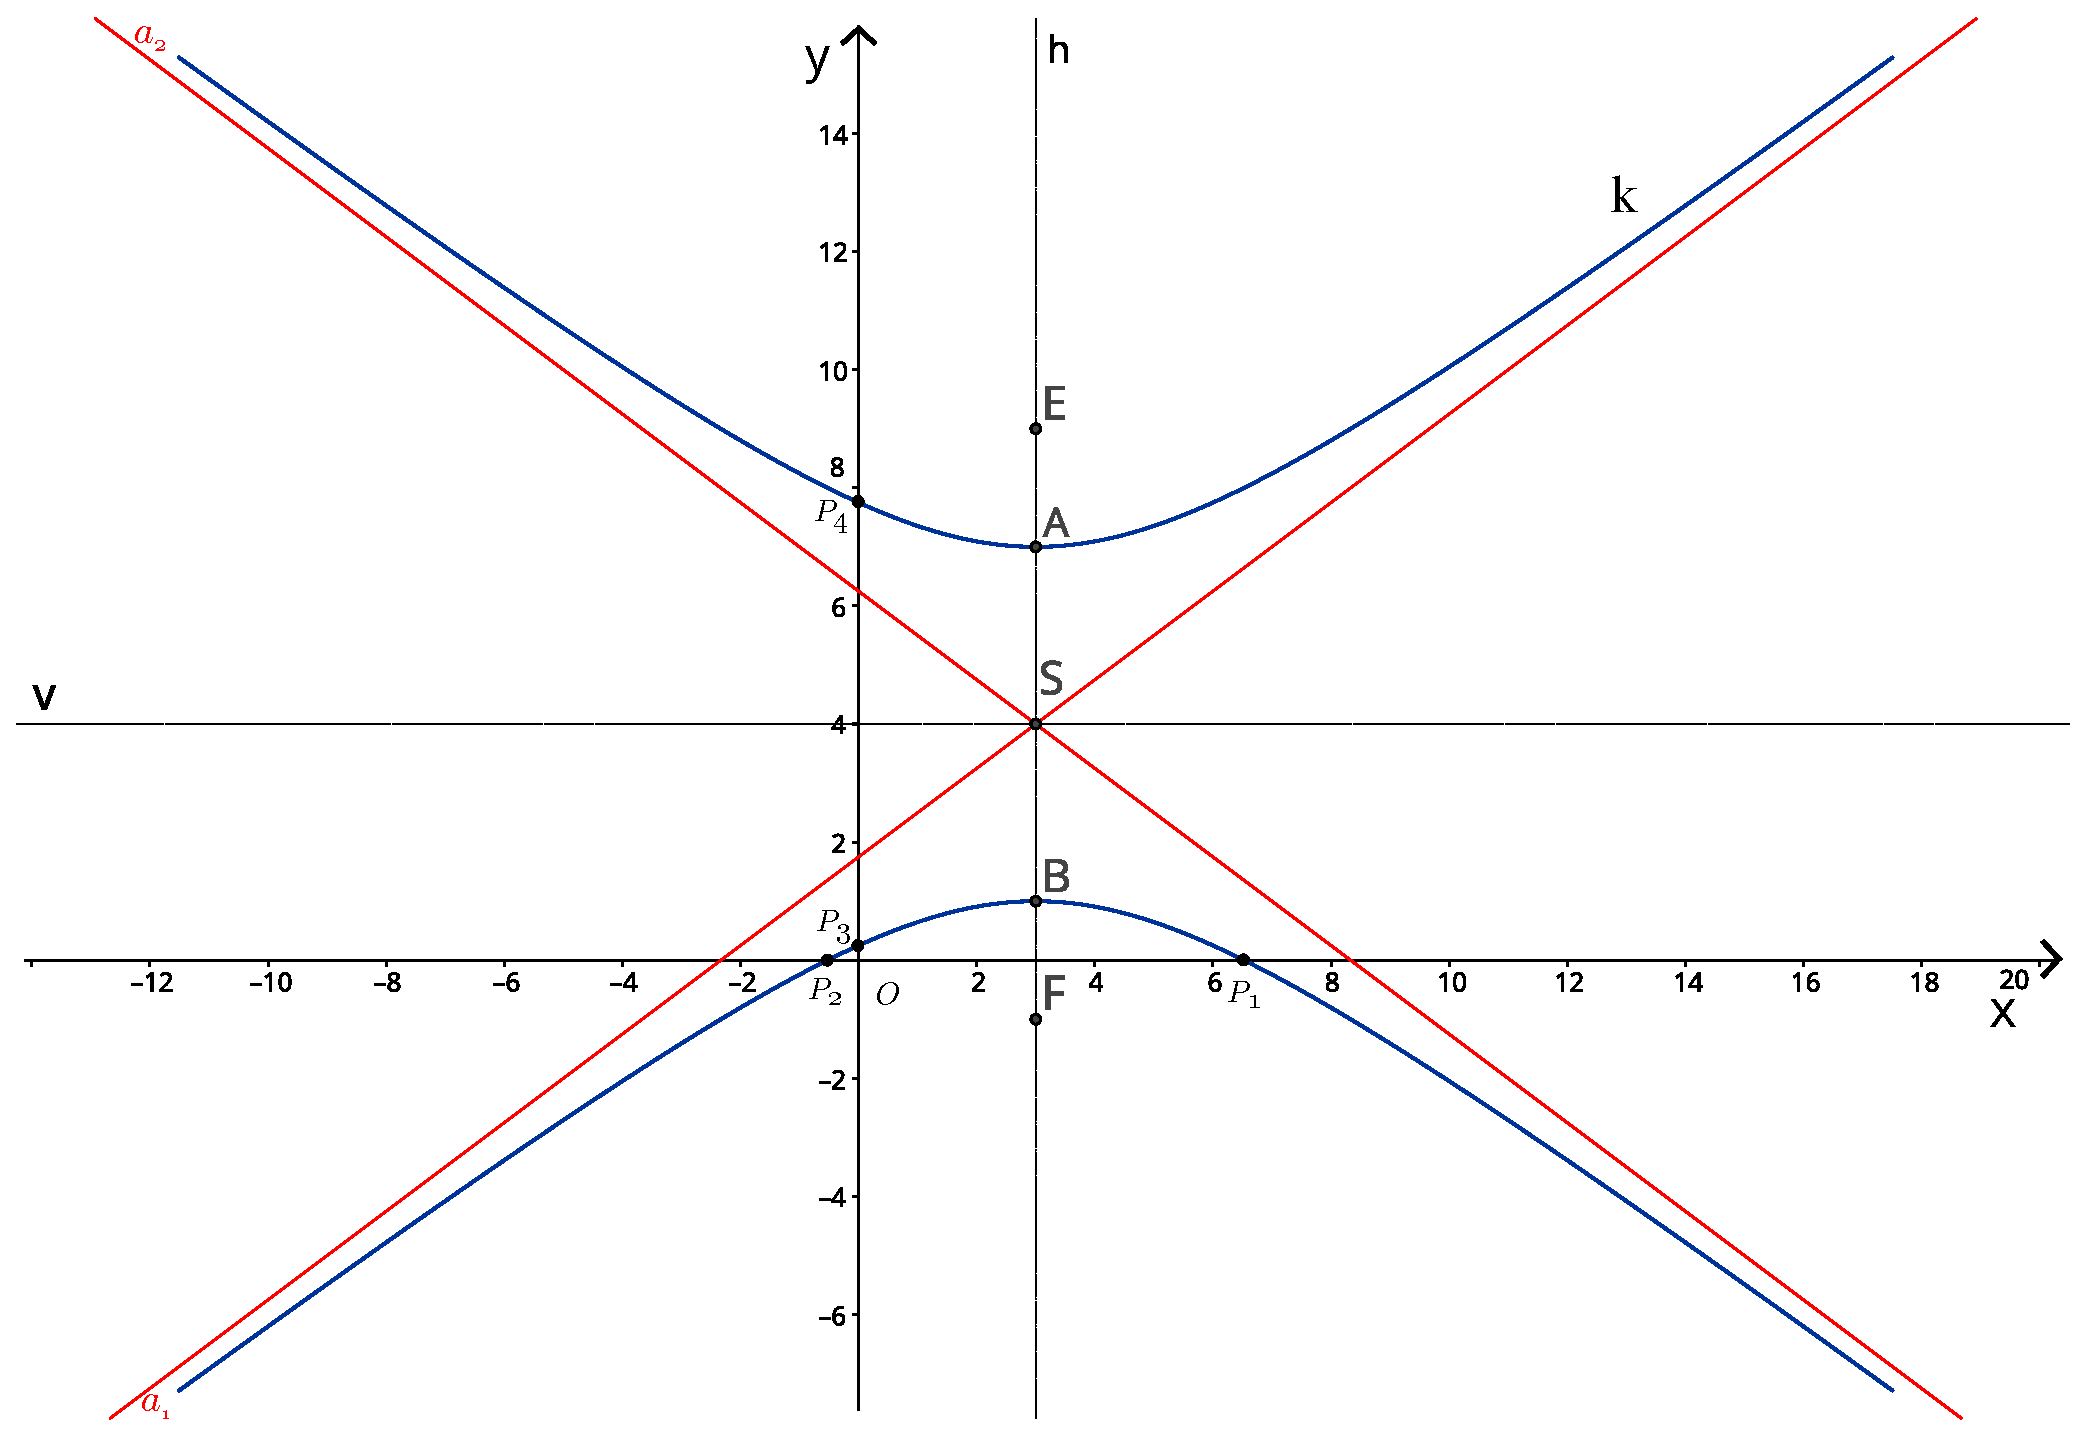
\includegraphics[width=\textwidth]{hyperbola2.eps}
				\caption{Hyperbola pro $t \in \langle-2, 2\rangle$}
									
			\end{figure}
\chapter{Další rovinné křivky}
Nyní si můžeme definovat nejrůznější křivky sami. \\
Např. $k(t)=[t, \cos{t}], t \in \langle0, 2\pi\rangle$ je část (1 perioda) grafu funkce $\cos$,  \\
$k(t)=[\cos{t}, \cos{t}], t \in \langle0, 2\pi\rangle$ je úsečka, která leží na přímce $y=x$, \\
$k(t)=\left[\frac{1}{t}, 1-t\right], t \in (-\infty, 0) \cup (0, +\infty)$ je rovnoosá hyperbola se středem $S=[0,1]$. \\[10pt]
	Mnoho křivek je známo, některé mají i své názvy a nebo se po někom jmenují. Než si některé z nich ukážeme, zavedeme si pojmy
	\textit{singulární bod křivky} a \textit{uzlový bod křivky}. \\[10pt]
	\textbf{Singulární bod křivky} je takový bod $K=k(t_0)$, ve kterém neexistuje tečna. To nastane tehdy, když neexistuje některá
	z derivací $x'(t_0)$, $y'(t_0)$ ($k'(t)=(x'(t), y'(t))$ je tečný vektor) nebo tečný vektor je nulový, tj. $k'(t_0)=(0,0)$. \\
	Už jsme poznamenali, že délka tečného vektoru vypovídá o rychlosti, s jakou je křivka v daném bodě probíhána. Pokud je $k'(t_0)=(0,0)$,
	dojde při probíhání křivky v bodě $K=k(t_0)$ k zastavení. \\[5pt]
	\textbf{Uzlový bod křivky} je bod, kterým křivka projde vícekrát a tečny v tomto bodě jsou různé.
	\begin{figure}[H]
		\centering
		\begin{subfigure}[b]{0.4\textwidth}
			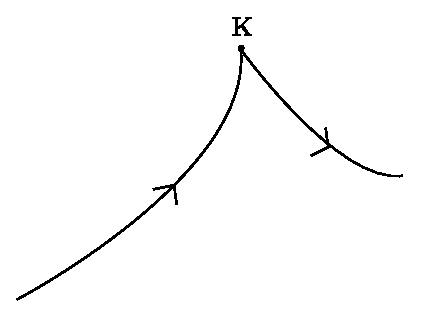
\includegraphics[width=\textwidth]{rovinnekrivky-teorie1.eps}
			\caption{Singulární bod}
		\end{subfigure}%
		\quad
		\begin{subfigure}[b]{0.4\textwidth}
			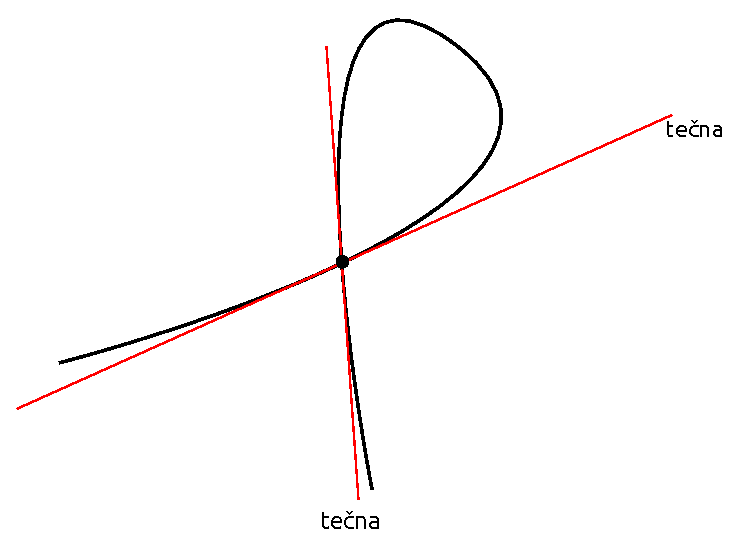
\includegraphics[width=\textwidth]{rovinnekrivky-teorie2.eps}
			\caption{Uzlový bod}
		\end{subfigure}%
	\end{figure}
	\clearpage
	\subsection*{Příklad 1}
	Je dána křivka 
	$$k(t) = \left[\cos{t} - \frac{\sqrt{2}}{2}\sin^2{t}, \cos{t}\sin{t}\right], t \in \langle0, 2\pi\rangle.$$
	Napište souřadnice singulárních bodů křivky. Dále napište parametrické i obecné rovnice tečen křivky
	v jejích průsečících s osou \textit{x}. \\[10pt]
	\textbf{Řešení:} Vypočítáme tečné vektory křivky \textit{k}, tj.:
	$$k'(t) = (-\sin{t}-\sqrt{2}\sin{t}\cos{t}, \cos^2{t}-\sin^2{t}).$$
	Abychom našli singulární body, řešíme soustavu
	$$-\sin{t}-\sqrt{2}\sin{t}\cos{t}=0$$
	a zároveň
	$$\cos^2{t}-\sin^2{t}=0.$$
	Můžeme najít všechna řešení rovnic na intervalu $\langle0,2\pi\rangle$ a pak udělat průnik.
	Nebo můžeme najít všechna řešení jedné rovnice na intervalu $\langle0,2\pi\rangle$ a vybrat
	z nich ta řešení, která splňují i druhou rovnici (ověříme dosazením).\\
	Jednodušší je použít druhý způsob. \\
	Vybereme rovnici
	\begin{align*}
		-\sin{t}-\sqrt{2}\sin{t}\cos{t} & = 0  \\
		-\sin{t}(1+\sqrt{2}\cos{t})     & = 0, 
	\end{align*}
	buď $\sin{t} = 0$ nebo $\cos{t}=-\frac{\sqrt{2}}{2}$.
	Všechna řešení na intervalu $\langle0,2\pi\rangle$ jsou
	$$t \in \left\{ 0, \frac{3\pi}{4}, \pi, \frac{5\pi}{4}, 2\pi \right\}.$$
	Dosazujeme postupně do rovnice $\cos^2{t}-\sin^2{t}=0$. Této rovnici vyhovují pouze
	$t_1 = \frac{3\pi}{4}$ a $t_2 = \frac{5\pi}{4}$. Singulární body jsou body
	\begin{align*}
		S_1 & = k\left(\frac{3\pi}{4}\right) = \left[-\frac{3\sqrt{2}}{4},-\frac{1}{2}\right]. \\
		S_2 & = k\left(\frac{5\pi}{4}\right) = \left[-\frac{3\sqrt{2}}{4},\frac{1}{2}\right].  
	\end{align*}
	Průsečíky s osou \textit{x} ($y=0$) vypočítáme z parametrického vyjádření křivky \textit{k}.
	$$\cos{t}\cdot\sin{t} = 0$$
	$$t\in\left\{0, \frac{\pi}{2}, \pi, \frac{3\pi}{2}, 2\pi\right\}$$
	Průsečíky křivky \textit{k} s osou \textit{x} jsou 3 body
	\begin{align*}
		P_1 & = k(\pi) = [-1,0],                                                                                 \\
		P_2 & = k\left(\frac{\pi}{2}\right) = k\left(\frac{3\pi}{2}\right) = \left[-\frac{\sqrt{2}}{2},0\right], \\
		P_3 & = k(0) = [1,0] = k(2\pi).                                                                          
	\end{align*}
	Vypočítáme tečné vektory a napíšeme rovnici tečen:
	\small
	\begin{flalign*}
		&k(\pi) = [-1.0], &\\
		&k'(\pi) = (0,1), &\\
		&p_1(s) = [-1, s],s \in \mathbb{R}\text{ parametrická rovnice}, &\\
		&p_1: x=-1\text{ obecná rovnice}, &\\
		&k\left(\frac{3\pi}{2}\right) = \left[-\frac{\sqrt{2}}{2},0\right], &\\
		&k'\left(\frac{3\pi}{2}\right) = (1,-1), &\\
		&p_2(s) = \left[-\frac{\sqrt{2}}{2}+s,-s\right],s \in \mathbb{R}, &\\
		&p_2: x+y+\frac{\sqrt{2}}{2}=0, &\\
		&k\left(\frac{\pi}{2}\right) = \left[-\frac{\sqrt{2}}{2},0\right], &\\
		&k'\left(\frac{\pi}{2}\right) = (-1,-1) \sim (1,1), &\\
		&q_2(s) = \left[-\frac{\sqrt{2}}{2}+s,s\right],s \in \mathbb{R}, &\\
		&q_2: x-y+\frac{\sqrt{2}}{2}=0,\\
	\end{flalign*}
	bod $\left[-\frac{\sqrt{2}}{2}, 0\right]$ je uzlový bod křivky \textit{k}, \\
	\begin{flalign*}
		&k(0) = [1,0] = k(2\pi), &\\
		&k'(0) = k'(2\pi) = (0,1), &\\
		&p_3(s) = [1, s],s \in \mathbb{R}, &\\
		&p_3: x=1. &\\
	\end{flalign*}	 
	\normalsize
	Nakreslíme-li zadanou křivku, vidíme na obrázku singulární body (špičky) i uzlový bod. Je také jasné
	proč se křivka nazývá \uv{ryba} (\textit{fish curve}).
	\begin{figure}[H]
		\centering
		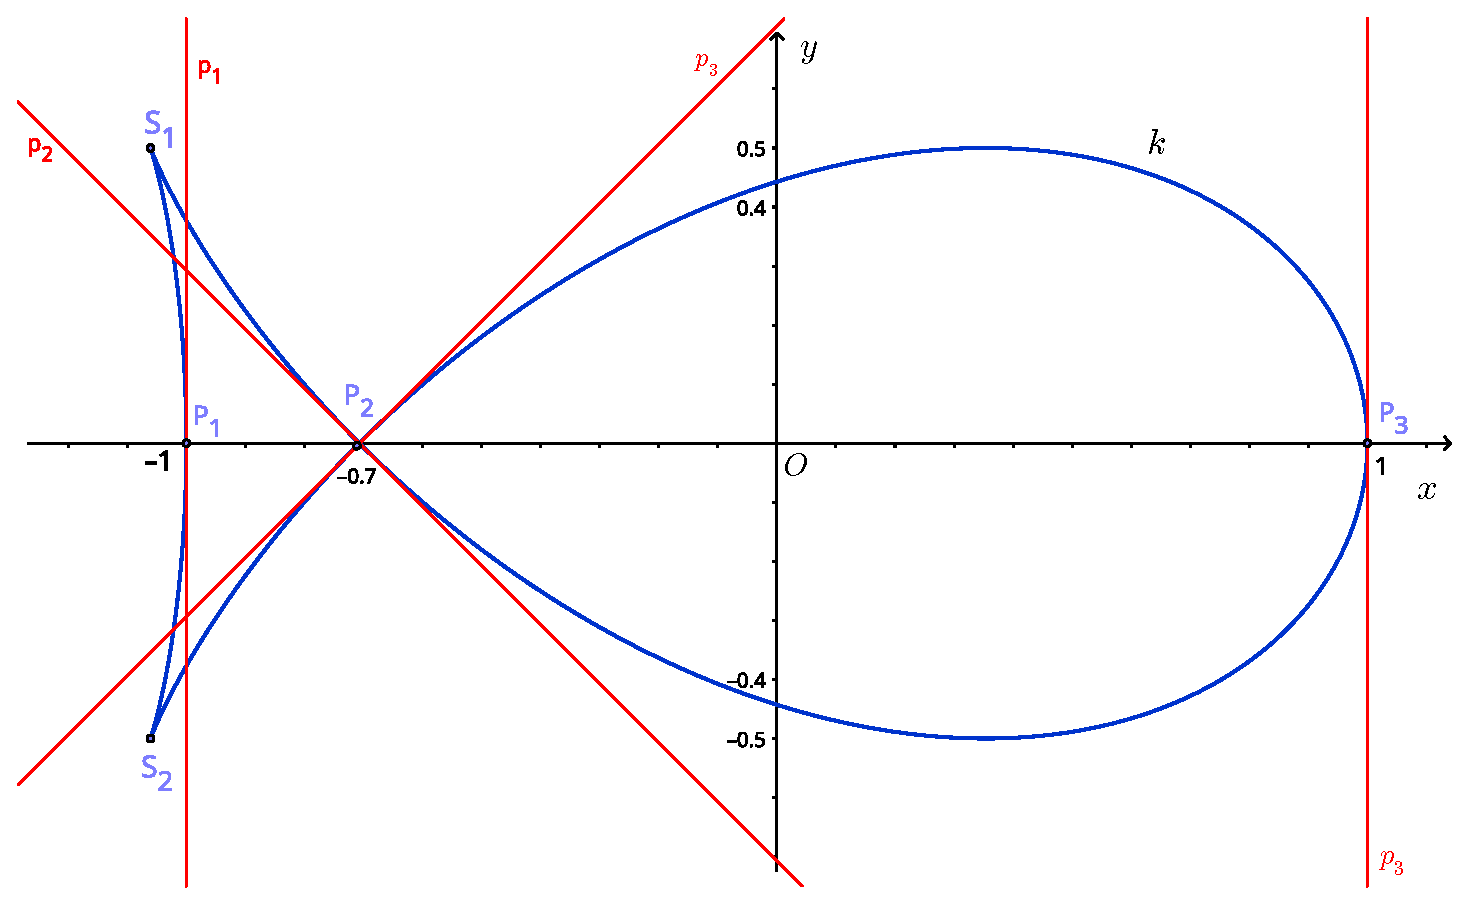
\includegraphics[width=\textwidth]{rovinnakrivka1-geo.eps}
		\caption{Fish curve pro $t \in \langle0, 2\pi\rangle$}
		
	\end{figure}
	\clearpage 		 
	\subsection*{Příklad 2}
	Je dána křivka
	$$k(t) = [16\sin^3{t}, 13\cos{t}-5\cos{2t}-2\cos{3t}-\cos{4t}], t \in \langle0, 2\pi\rangle.$$
	Napište souřadnice singulárních bodů křivky. Dále napište souřadnice bodů křivky, ve kterých
	má křivka tečny rovnoběžné s osou \textit{y}, napište obecné rovnice těchto tečen. \\[10pt]
	\textbf{Řešení:} Vypočítáme tečné vektory křivky \textit{k}, tj.:
	$$k'(t) = (48\sin^2{t}\cos{t},-13\sin{t}+10\sin{2t}+6\sin{3t}+4\sin{4t}).$$
	Abychom našli singulární body, řešíme soustavu rovnic
	$$48\sin^2{t}\cos{t}=0$$
	a zároveň
	$$-13\sin{t}+10\sin{2t}+6\sin{3t}+4\sin{4t}=0.$$
	Najdeme všechna řešení první rovnice na intervalu $\langle0, 2\pi\rangle$, jsou to
	$t \in \left\{ 0, \frac{\pi}{2}, \pi, \frac{3\pi}{2}, 2\pi \right\}$. \\
	Tato řešení dosazujeme do druhé rovnice, druhé rovnici vyhovují 3 hodnoty
	$t_1=0$, $t_2=\pi$ a $t_3=2\pi$. \\
	Křivka má dva singulární body:
	\begin{align*}
		S_1 & = k(0) = k(2\pi)=[0, 5], \\
		S_2 & = k(\pi) = [0, -17].     
	\end{align*}
	Tečný vektor je rovnoběžný s osou \textit{y}, je-li jeho první složka nulová a druhá nenulová.
	To nastane pro hodnoty $t_4=\frac{\pi}{2}$ a $t_5=\frac{3\pi}{2}$.
	Obecné rovnice tečen rovnoběžných s osou \textit{y} jsou:
	\begin{align*}
		k\left(\frac{3\pi}{2}\right)  & = [-16,4] = P_1, \\
		k'\left(\frac{3\pi}{2}\right) & = (0, 19),       \\
		p_1: x                        & = -16            
	\end{align*}
	a
	\begin{align*}
		k\left(\frac{\pi}{2}\right)  & = [16,4] = P_2, \\
		k'\left(\frac{\pi}{2}\right) & = (0, -19),     \\
		p_2: x                       & = 16.           
	\end{align*}
	\clearpage
	\noindent Nakreslíme-li zadanou křivku, vidíme na obrázku singulární body (špičky na křivce). Tato křivka se nazývá \uv{srdce} (\textit{heartcurve}) a řadíme ji mezi další křivky, které se často souhrnně označují \textit{srdcovky}.
	\begin{figure}[H]
		\centering
		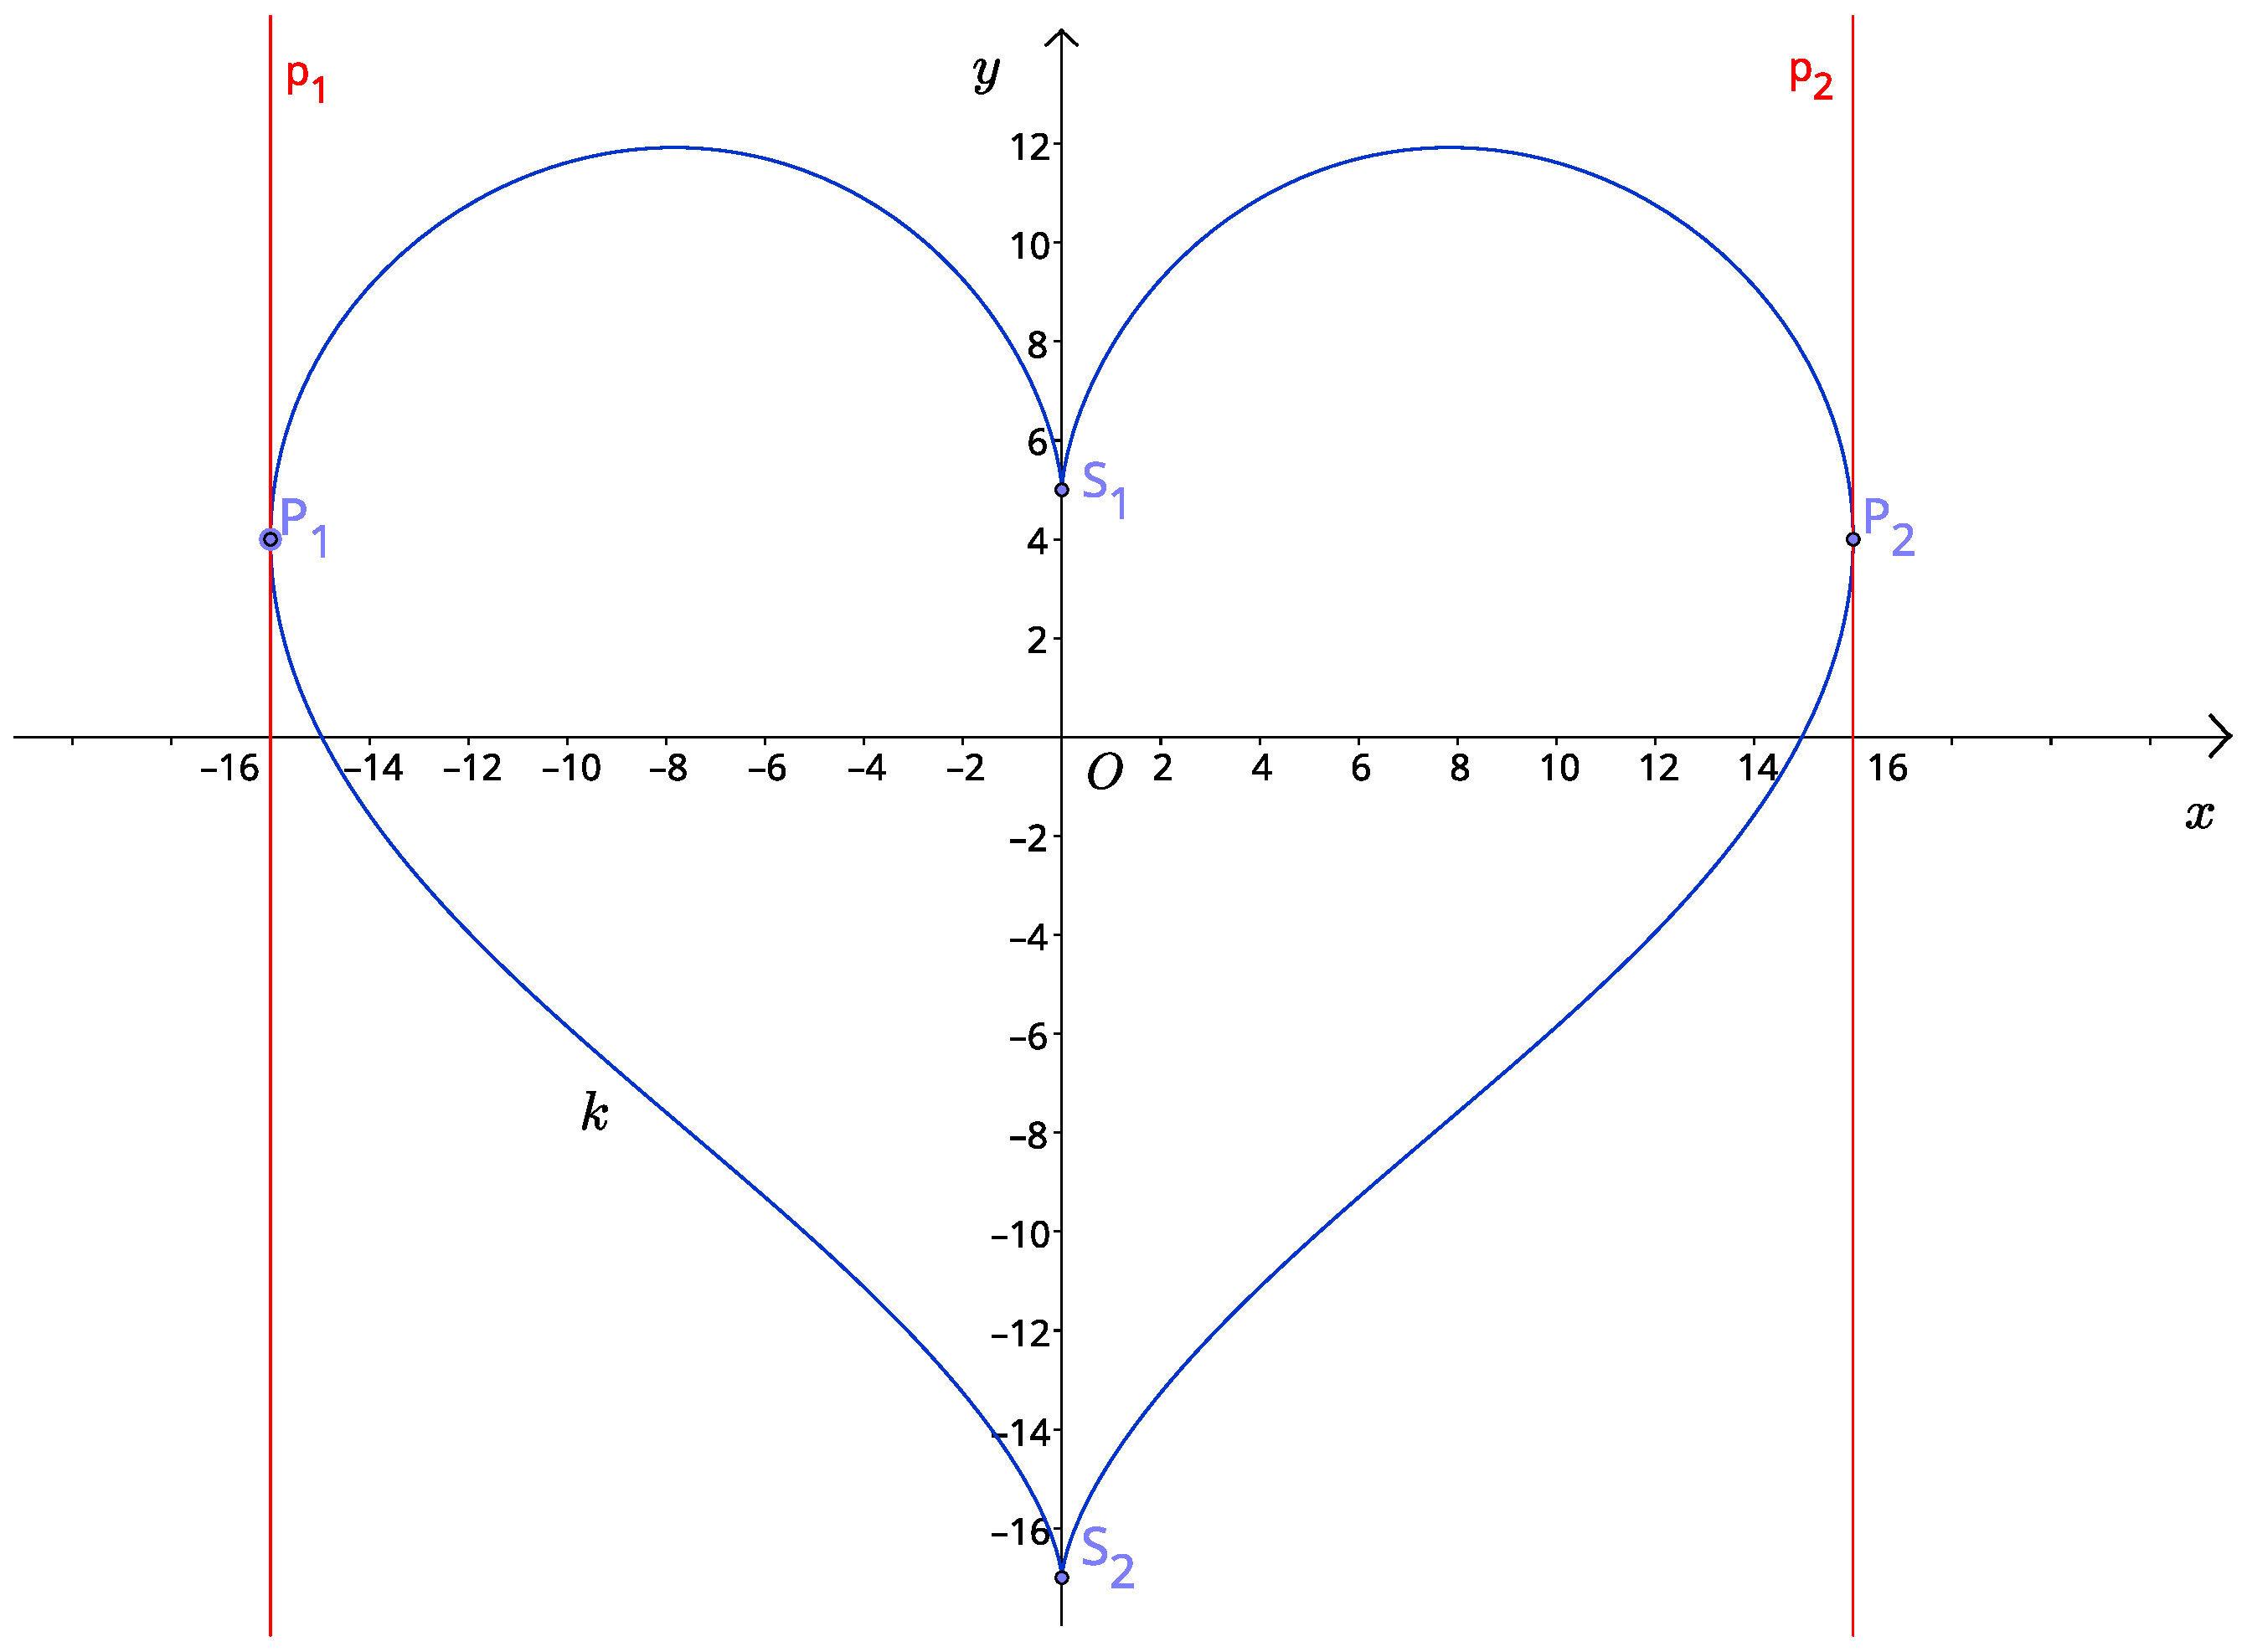
\includegraphics[width=\textwidth]{rovinnakrivka2-geo.eps}
		\caption{Rovinná křivka pro $t \in \langle0, 2\pi\rangle$}
		
	\end{figure}	
\chapter{Šroubovice}
Nyní se budeme věnovat prostorovým křivkám. Nejčastěji se v praxi používá šroubovice na válcové ploše. \\
Abychom mohli popsat šroubovici bodu, musíme zadat \textit{šroubový pohyb}. \\[5pt]
\textbf{Šroubový pohyb} je dán
\begin{enumerate}
	\item osou \textit{o},
	\item smyslem (pravotočivý a levotočivý),
	\item výškou závitu v.
\end{enumerate}
Osa šroubového pohybu může být libovolná přímka v prostoru, pro zjednodušení budeme v dalším textu používat osu \textit{z}
souřadné soustavy $(O, x, y, z)$. Používáme vždy \textit{pravotočivou} kartézskou souřadnou soustavu, kterou využívají i grafické
programy. \\
Šroubový pohyb je složením rovnoměrného rotačního pohybu a rovnoměrného translačního pohybu. \\
Pokud je rotační pohyb proti směru hodinových ručiček a translační pohyb ve směru kladné poloosy osy \textit{z} nebo rotační pohyb
ve směru hodinových ručiček a translační pohyb ve směru záporné poloosy osy \textit{z}, je šroubový pohyb pravotočivý, v opačném
případě je levotočivý.
\begin{figure}[H]
	\centering
	\begin{subfigure}[b]{0.4\textwidth}
		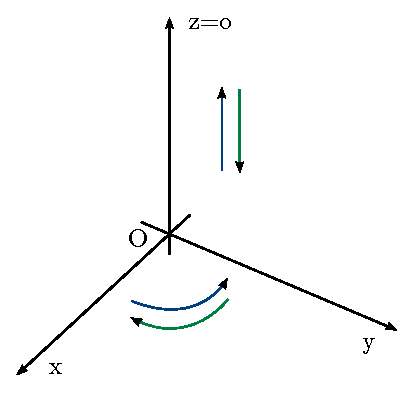
\includegraphics[width=\textwidth]{sroubovice-teorie1.eps}
		\caption{Pravotočivý šroubový pohyb}
	\end{subfigure}%
	\quad
	\begin{subfigure}[b]{0.4\textwidth}
		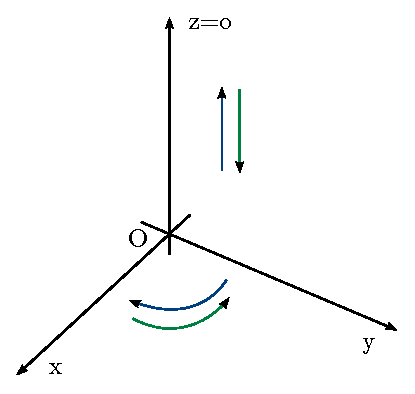
\includegraphics[width=\textwidth]{sroubovice-teorie2.eps}
		\caption{Levotočivý šroubový pohyb}
	\end{subfigure}%
\end{figure}
\clearpage
\noindent Vyberme si bod \textit{A} v prostoru, který neleží na ose šroubového
pohybu. Bod se při šroubovém pohybu rovnoměrně otáčí kolem osy \textit{o} a zároveň se rovnoměrně posunuje ve směru osy \textit{o}.
Šroubovice bodu \textit{A} leží na válcové ploše, jejíž osou je osa \textit{o} šroubového pohybu a poloměr je roven vzdáleností bodu \textit{A} od osy \textit{o}. \\
Výška závitu \textit{v} je vzdálenost bodu $A$ a bodu $A'$, kde $A$ a $A'$ jsou body na povrchové přímce \textit{p} válcové plochy
a mezi nimi není žádný jiný bod šroubovice. Část šroubovice mezi body $A$ a $A'$ je tzv. 1 závit šroubovice a odpovídá otočení o
úhel $2\pi$.
\begin{figure}[H]
	\centering
	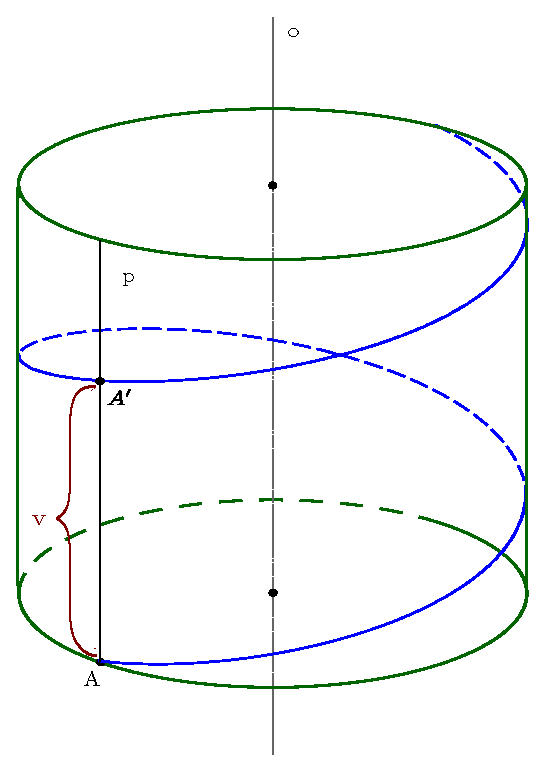
\includegraphics[width=0.3\textwidth]{sroubovice-teorie3.eps}
	\caption{Šroubovice na válcové ploše}
\end{figure}
\noindent{}Po rozstřižení válcové plochy podél \textit{p} a rozvinutí do roviny máme následující obrázek.
\begin{figure}[H]
	\centering
	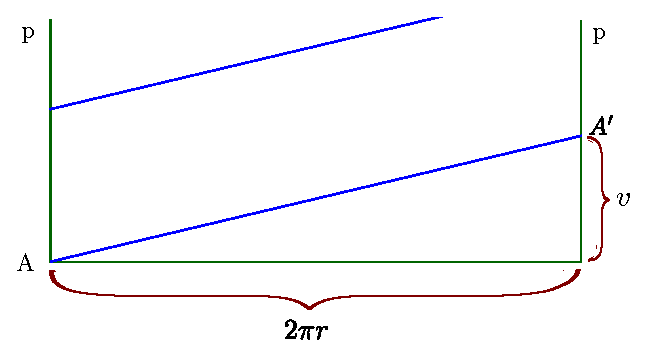
\includegraphics[width=0.8\textwidth]{sroubovice-teorie4.eps}
	\caption{Válcová plocha rozstřižená podél přímky \textit{p} a rozvinutá do roviny}
\end{figure}
\noindent{}To je také návodem, jak si snadno šroubovici \uv{vyrobit}. Stačí slepit papír, na kterém jsme narýsovali úsečku pro jeden závit nebo více
rovnoběžných úseček pro více závitů. \\
V technické praxi se často užívá místo výšky závitu tzv. \textit{redukovaná výška závitu}, kterou značíme $v_0$. Je to výška posunutí
odpovídající otočení o úhel 1 radián (přibližně $57^{\circ}17'45''$). Úhlu 1 radián odpovídá délka oblouku kružnice rovná poloměru \textit{r} kružnice. \\
Z obrázku
\begin{figure}[H]
	\centering
	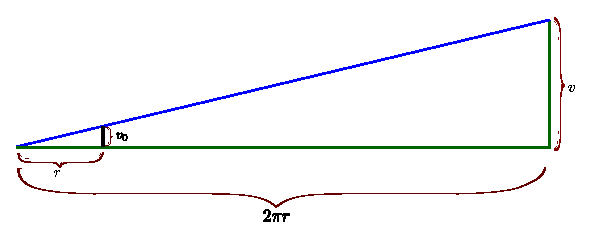
\includegraphics[width=0.8\textwidth]{sroubovice-teorie5.eps}
	\caption{Ilustrační obrázek}
\end{figure}
\noindent snadno odvodíme vztah mezi výškou \textit{v} závitu a redukovanou výškou $v_0$:
\begin{align*}
	\frac{v_0}{r} & = \frac{v}{2 \pi r} \\
	v_0           & = \frac{v}{2\pi}    
\end{align*}
Jak napsat parametrické vyjádření šroubovice bodu $A=[a_1, a_2, a_3]$? \\
Zadejme šroubový pohyb:
\begin{enumerate}
	\item osa \textit{o} je souřadnicová osa \textit{z},
	\item pravotočivý (resp. levotočivý),
	\item výškou závitu je \textit{v} (nebo redukovaná výška je $v_0$).
\end{enumerate}
Šroubovice leží na válcové ploše, jejíž osou je osa \textit{z}. Průnik této plochy s půdorysnou $(x, y)$ je kružnice.
Začneme parametrickým popisem kružnice v rovině $(x, y)$, střed kružnice je bod $[0,0]$ a kružnice prochází bodem $[a_1, a_2]$. \\
Je-li šroubový pohyb \emph{pravotočivý}, musíme kružnici popsat tak, aby byla probíhána \emph{proti} směru hodinových ručiček, tj. v kladném směru.
Navíc požadujeme, aby pro $t=0$ byl výchozí bod $[a_1, a_2]$. \\
Je-li šroubový pohyb levotočivý, musíme kružnici popsat tak, aby byla probíhána ve směru hodinových ručiček, tj. v záporném směru. Opět v čase $t=0$
jsme v bodě $[a_1, a_2]$. Tedy
\begin{align*}
	m(t) & = [a_1\cos{t}-a_2\sin{t}, a_2\cos{t}+a_1\sin{t}] \text{ pro kladný směr},   \\
	m(t) & = [a_1\cos{t}+a_2\sin{t}, a_2\cos{t}-a_1\sin{t}] \text{ pro záporný směr}. 
\end{align*}
Třetí \textit{z}-ová souřadnice se týká posunutí, parametrický popis pravotočivé šroubovice je
$$k(t) = [a_1\cos{t}-a_2\sin{t}, a_2\cos{t}+a_1\sin{t}, a_3+v_0 t], t \in \mathbb{R}.$$
Parametrický popis levotočivé šroubovice je
$$k(t) = [a_1\cos{t}+a_2\sin{t}, a_2\cos{t}-a_1\sin{t}, a_3+v_0 t], t \in \mathbb{R}.$$
Šroubovice je neomezená křivka v obou směrech. \\
Důležitý je jeden závit šroubovice, který se dále jen posunuje. Pokud chceme popsat 1 závit, bereme parametr \textit{t} z intervalu délky $2\pi$.
Použijeme-li výše uvedený parametrický popis, je $k(0)=A$ a pro jeden závit s krajním bodem \textit{A} bereme $t\in\langle0, 2\pi\rangle$.
\clearpage
\subsection*{Příklad 1}
Napište parametrické vyjádření šroubovice bodu $A=[0,4,0]$. Osa šroubového pohybu je osa \textit{z}, šroubový pohyb je
\begin{enumerate}
	\item pravotočivý
	\item levotočivý
\end{enumerate}
Výška závitu $v=12$. \\[10pt]
\textbf{Řešení: } \\
\begin{enumerate}
	\item Popíšeme kružnici \textit{m} v rovině $(x,y)$, střed je bod $[0,0]$, výchozí bod je bod $[x_A, y_A]=[0,4]$, kružnice je probíhána v kladném směru:
	      $$m(t) = \left[-4\sin{t}, 4\cos{t}\right].$$
	      Pro popis pravotočivé šroubovice doplníme \textit{z}-ovou souřadnici $z_A+v_0t$, kde $v_0=\frac{v}{2\pi}=\frac{12}{2\pi}=\frac{6}{\pi}$:
	      $$k(t) = \left[-4\sin{t}, 4\cos{t}, \frac{6}{\pi}t\right], t \in \mathbb{R},$$
	      (nebo $t \in \langle0, 2\pi\rangle$ pro 1 závit šroubovice).
	\item Parametrický popis levotočivé šroubovice získáme z předchozího popisu změnou znaménka u funkce $\sin$ (oběh kružnice v záporném směru):
	      $$k(t) = \left[4\sin{t}, 4\cos{t}, \frac{6}{\pi}t\right], t \in \mathbb{R},$$
	      (nebo $t \in \langle0, 2\pi\rangle$ pro 1 závit). 	
	      \clearpage
	      \begin{figure}[H]
	      	\centering
	      	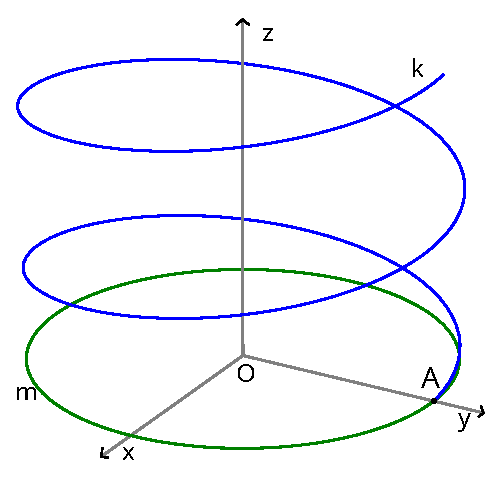
\includegraphics[width=0.5\textwidth]{sroubovice1.eps}
	      	\caption{Pravotočivá šroubovice pro $t \in \langle0, 4\pi\rangle$}
	      \end{figure}	
	      \begin{figure}[H]
	      	\centering
	      	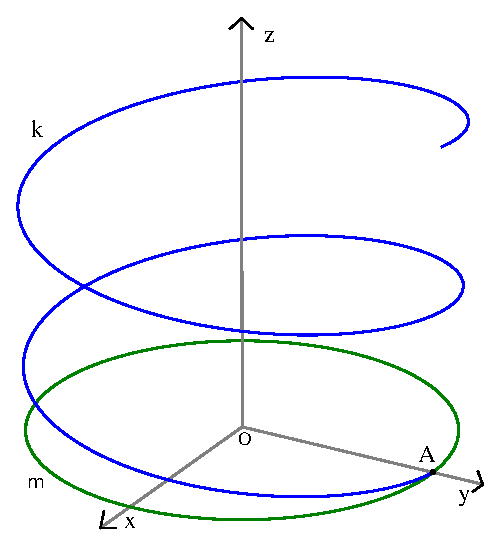
\includegraphics[width=0.5\textwidth]{sroubovice2.eps}
	      	\caption{Levotočivá šroubovice pro $t \in \langle0, 4\pi\rangle$}
	      	
	      \end{figure}	 	
\end{enumerate}
\clearpage
\subsection*{Příklad 2}
Napište parametrické vyjádření šroubovice bodu $A=[-4,0,0]$. Osa šroubového pohybu je osa \textit{z},
šroubový pohyb je
\begin{enumerate}
	\item pravotočivý
	\item levotočivý
\end{enumerate}
Výška závitu je $v=18$. \\[10pt]
\textbf{Řešení: } 
\begin{enumerate}
	\item Popíšeme kružnici v rovině $(x,y)$, střed je bod $[0,0]$, výchozí bod je bod $[x_A, y_A]=[-4,0]$, kružnice je probíhána v kladném směru:
	      $$m(t) = \left[-4\cos{t}, -4\sin{t}\right].$$
	      Pro popis pravotočivé šroubovice doplníme \textit{z}-ovou souřadnici $z_A+v_0t$, kde $v_0=\frac{v}{2\pi}=\frac{18}{2\pi}=\frac{9}{\pi}$:
	      $$k(t) = \left[-4\cos{t}, -4\sin{t}, \frac{9}{\pi}t\right], t \in \mathbb{R},$$
	      (nebo $t \in \langle0, 2\pi\rangle$ pro 1 závit šroubovice).
	      \begin{figure}[H]
	      	\centering
	      	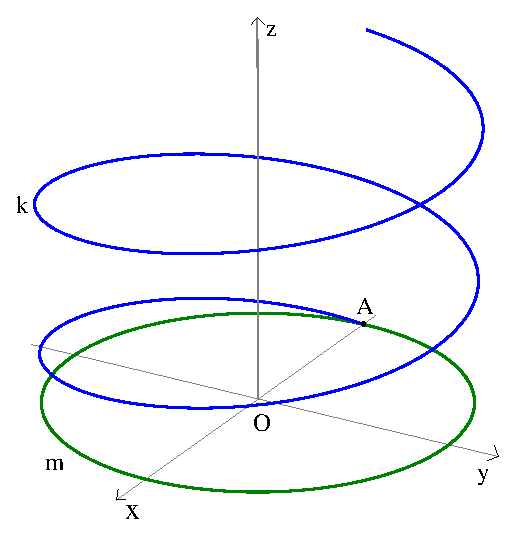
\includegraphics[width=0.5\textwidth]{sroubovice3.eps}
	      	\caption{Pravotočivá šroubovice pro $t \in \langle0, 4\pi\rangle$}
	      	
	      \end{figure}	 	
	\item Parametrický popis levotočivé šroubovice získáme z předchozího popisu změnou znaménka u funkce $\sin$ (oběh kružnice v záporném směru):
	      $$k(t) = \left[-4\cos{t}, 4\sin{t}, \frac{9}{\pi}t\right], t \in \mathbb{R},$$
	      (nebo $t \in \langle0, 2\pi\rangle$ pro 1 závit). 	
	      \begin{figure}[H]
	      	\centering
	      	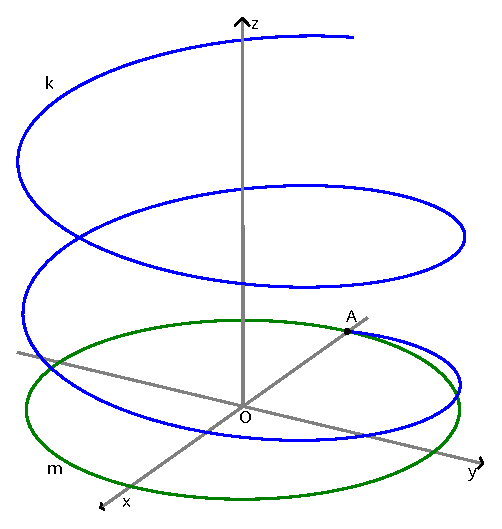
\includegraphics[width=0.5\textwidth]{sroubovice4.eps}
	      	\caption{Levotočivá šroubovice pro $t \in \langle0, 4\pi\rangle$}
	      	
	      \end{figure}	 	
\end{enumerate}
\clearpage
\subsection*{Příklad 3}
Napište parametrické vyjádření šroubovice bodu $A=[0,-4,0]$. Osa šroubového pohybu je osa \textit{z},
šroubový pohyb je
\begin{enumerate}
	\item pravotočivý
	\item levotočivý
\end{enumerate}
Redukovaná výška závitu je $v_0=3$. \\[10pt]
\textbf{Řešení: } 
\begin{enumerate}
	\item Popíšeme kružnici v rovině $(x,y)$, střed je bod $[0,0]$, výchozí bod je bod $[x_A, y_A]=[0,-4]$, kružnice je probíhána v kladném směru:
	      $$m(t) = \left[4\sin{t}, -4\cos{t}\right].$$
	      Pro popis pravotočivé šroubovice doplníme \textit{z}-ovou souřadnici $z_A+v_0t$:
	      $$k(t) = \left[4\sin{t}, -4\cos{t}, 3t\right], t \in \mathbb{R},$$
	      (nebo $t \in \langle0, 2\pi\rangle$ pro 1 závit šroubovice).
	      \begin{figure}[H]
	      	\centering
	      	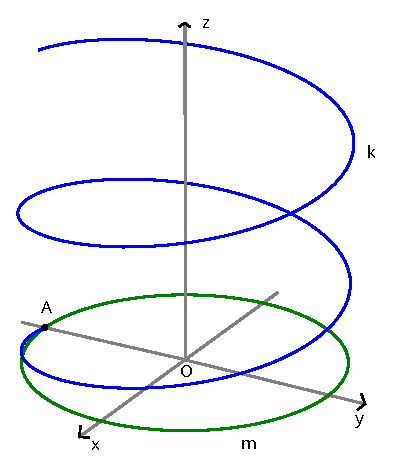
\includegraphics[width=0.5\textwidth]{sroubovice5.eps}
	      	\caption{Pravotočivá šroubovice pro $t \in \langle0, 4\pi\rangle$}
	      	
	      \end{figure}	 	
	      \clearpage
	\item Parametrický popis levotočivé šroubovice získáme z předchozího popisu změnou znaménka u funkce $\sin$ (oběh kružnice v záporném směru):
	      $$k(t) = \left[-4\sin{t}, -4\cos{t}, 3t\right], t \in \mathbb{R},$$
	      (nebo $t \in \langle0, 2\pi\rangle$ pro 1 závit). 	
	      \begin{figure}[H]
	      	\centering
	      	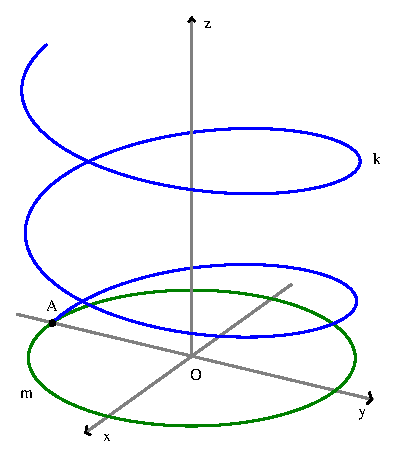
\includegraphics[width=0.5\textwidth]{sroubovice6.eps}
	      	\caption{Levotočivá šroubovice pro $t \in \langle0, 4\pi\rangle$}
	      	
	      \end{figure}	 	
\end{enumerate}
\clearpage
\subsection*{Příklad 4}
Napište parametrické vyjádření šroubovice bodu $A=[4,0,3]$. Osa šroubového pohybu je osa \textit{z},
šroubový pohyb je
\begin{enumerate}
	\item pravotočivý
	\item levotočivý
\end{enumerate}
Redukovaná výška závitu je $v_0=2$. \\
Dále popište tečnu šroubovice v bodě \textit{A}. \\[10pt]
\textbf{Řešení: } 
\begin{enumerate}
	\item Popíšeme kružnici v rovině $(x,y)$, střed je bod $[0,0]$, výchozí bod je bod $[x_A, y_A]=[4,0]$, kružnice je probíhána v kladném směru:
	      $$m(t) = \left[4\cos{t}, 4\sin{t}\right].$$
	      Pro popis pravotočivé šroubovice doplníme \textit{z}-ovou souřadnici $z_A+v_0t$:
	      $$k(t) = \left[4\cos{t}, 4\sin{t}, 2t+3\right], t \in \mathbb{R},$$
	      (nebo $t \in \langle0, 2\pi\rangle$ pro 1 závit šroubovice). \\
	      Tečné vektory získáme derivováním
	      $$k'(t)=(-4\sin{t}, 4\cos{t}, 2).$$
	      Pro bod $A=k(0)$ je tečný vektor
	      $$k'(0)=(0,4,2)$$
	      a parametrický popis tečny \textit{p} je
	      $$p(s)=[4,4s,3+2s], s \in \mathbb{R}.$$
	\item Parametrický popis levotočivé šroubovice získáme z předchozího popisu změnou znaménka u funkce $\sin$ (oběh kružnice v záporném směru):
	      $$k(t) = \left[4\cos{t}, -4\sin{t}, 2t+3\right], t \in \mathbb{R},$$
	      (nebo $t \in \langle0, 2\pi\rangle$ pro 1 závit). 	\\
	      Tečné vektory získáme derivováním
	      $$k'(t)=(-4\sin{t}, -4\cos{t}, 2).$$
	      Pro bod $A=k(0)$ je tečný vektor
	      $$k'(0)=(0,-4,2)$$
	      a parametrický popis tečny \textit{p} je
	      $$p(s)=[4,-4s,3+2s], s \in \mathbb{R}.$$
	      \begin{figure}[H]
	      	\centering
	      	\includegraphics[width=0.5\textwidth]{sroubovice7.eps}
	      	\caption{Pravotočivá šroubovice pro $t \in \langle0, 2\pi\rangle$}
	      \end{figure}	 	
	      \begin{figure}[H]
	      	\centering
	      	\includegraphics[width=0.5\textwidth]{sroubovice8.eps}
	      	\caption{Levotočivá šroubovice pro $t \in \langle0, 2\pi\rangle$}
	      	
	      \end{figure}	 	
\end{enumerate}
\clearpage

\subsection*{Příklad 5}
Napište parametrické vyjádření šroubovice bodu $A=[3,4,2]$. Osa pravotočivého šroubového pohybu je osa \textit{z},
výška závitu je $v=20$. \\
Dále popište tečny šroubovice v bodech \textit{A}, $k\left(\frac{\pi}{2}\right)$, $k(\pi)$ a $k(2\pi)$.\\[10pt]
\textbf{Řešení: } 
Popíšeme kružnici v rovině $(x,y)$, střed je bod $[0,0]$, výchozí bod je bod $[x_A, y_A]=[3,4]$, kružnice je probíhána v kladném směru:
$$m(t) = \left[3\cos{t}-4\sin{t}, 4\cos{t}+3\sin{t}\right].$$
Pro popis pravotočivé šroubovice doplníme \textit{z}-ovou souřadnici $z_A+v_0t$, kde $v_0=\frac{v}{2\pi}=\frac{20}{2\pi}=\frac{10}{\pi}$:
$$k(t) = \left[3\cos{t}-4\sin{t}, 4\cos{t}+3\sin{t}, \frac{10}{\pi}t+2\right], t \in \mathbb{R},$$
(nebo $t \in \langle0, 2\pi\rangle$ pro 1 závit šroubovice). \\
Tečné vektory získáme derivováním
$$k'(t)=\left(-3\sin{t}-4\cos{t}, 3\cos{t}-4\sin{t}, \frac{10}{\pi}\right).$$
Konkrétní tečné vektory jsou tedy:
\begin{align*}
	k'(0)                        & =\left(-4,3,\frac{10}{\pi}\right),   \\
	k'\left(\frac{\pi}{2}\right) & = \left(-3,-4,\frac{10}{\pi}\right), \\
	k'(\pi)                      & = \left(4,-3,\frac{10}{\pi}\right),  \\
	k'(2\pi)                     & = \left(-4,3,\frac{10}{\pi}\right).  
\end{align*}
V bodech:
\begin{align*}
	k(0)                        & =A=\left[3,4,2\right],   \\
	k\left(\frac{\pi}{2}\right) & = \left[-4,3,7\right],   \\
	k(\pi)                      & = \left[-3,-4,12\right], \\
	k(2\pi)                     & = \left[3,4,22\right]    
\end{align*} 	
je parametrický popis tečen:
\begin{align*}
	p_1(s) & = \left[3-4s,4+3s,2+\frac{10}{\pi}s\right], s \in \mathbb{R},    \\
	p_2(s) & = \left[-4-3s,3-4s,7+\frac{10}{\pi}s\right], s \in \mathbb{R},   \\
	p_3(s) & = \left[-3+4s,-4-3s,12+\frac{10}{\pi}s\right], s \in \mathbb{R}, \\
	p_4(s) & = \left[3-4s,4+3s,22+\frac{10}{\pi}s\right], s \in \mathbb{R}.   
\end{align*} 	
\begin{figure}[H]
	\centering
	\includegraphics[width=0.7\textwidth]{sroubovice9-oprava.eps}
	\caption{Pravotočivá šroubovice pro $t \in \langle0, \frac{5\pi}{2}\rangle$}
	
\end{figure}	 	
\chapter{Další prostorové křivky}
Nyní si můžeme definovat nejrůznější křivky sami. Například
$$k(t)=[\cos{t}, \ln{t}\cdot\sin{t}, \ln{t}], t \in (0, +\infty),$$
\begin{figure}[H]
	\centering
	\includegraphics[width=0.275\textwidth]{prostorovekrivky-teorie1.eps}
	\caption{Křivka \textit{k} pro $t \in \left\langle\frac{1}{10}, 10\right\rangle$}
\end{figure}
$$k(t)=\left[\frac{1}{t^2+1}, \frac{t}{t^2+1}, \frac{t^2}{t^2+1}\right], t \in \mathbb{R},$$
\begin{figure}[H]
	\centering
	\includegraphics[width=0.28\textwidth]{prostorovekrivky-teorie2.eps}
	\caption{Křivka \textit{k} pro $t \in \langle-10,10\rangle$}
\end{figure}
(je to elipsa v rovině $x+z-1=0$), \clearpage{}
\noindent{}$$k(t)=[\sinh{t}, \cosh{t}, \sin{6t}], t \in \langle-\pi, \pi\rangle.$$
\begin{figure}[H]
	\centering
	\includegraphics[width=0.8\textwidth]{prostorovekrivky-teorie3.eps}
	\caption{Křivka \textit{k} pro $t \in \langle-\pi, \pi\rangle$}
\end{figure}
\noindent Stejně jako u rovinných křivek mohou na prostorových křivkách být singulární body nebo uzlové body. Tečný vektor v singulárním bodě $K(t_0)$ buď neexistuje nebo je nulový, tj.:
$$k'(t_0)=(0,0,0).$$
\clearpage
\subsection*{Příklad 1}
Je dána křivka
$$k(t) = [\cos^3{t}, \sin^3{t}, \cos{2t}], t \in \langle0, 2\pi\rangle.$$
Napište souřadnice singulárních bodů. Dále popište tečnu křivky v bodě $T=k\left(\frac{\pi}{6}\right)$. \\[10pt]
\textbf{Řešení:} Vypočítáme tečné vektory
$$k'(t)=(-3 \cos^2{t} \cdot \sin{t}, 3 \sin^2{t} \cdot \cos{t}, -2\sin{2t}).$$
Má-li být nějaký bod singulární, musí být tečný vektor nulový. \\
Řešíme soustavu rovnic na intervalu $\langle0,2\pi\rangle$:
\begin{align*}
	-3\cos^2{t}\sin{t} & = 0, \\
	3\sin^2{t}\cos{t}  & = 0, \\
	-2\sin{2t}         & = 0. 
\end{align*}
Můžeme najít řešení všech tří rovnic na intervalu $\langle0,2\pi\rangle$ a pak udělat průnik řešení. Výhodnější je
najít všechna řešení jedné rovnice na intervalu $\langle0,2\pi\rangle$ a do zbývajících 2 rovnic tato řešení dosadit.
Vybereme ta řešení, která vyhovují pro všechny rovnice. \\
Vybereme si poslední rovnici
\begin{align*}
	\sin{2t} & = 0              \\
	2t       & = k\pi           \\
	t        & = k\frac{\pi}{2} 
\end{align*}
Na intervalu $\langle0,2\pi\rangle$ máme 5 řešení
$$t \in \left\{0, \frac{\pi}{2}, \pi, \frac{3\pi}{2}, 2\pi\right\}$$
Všech 5 řešení vyhovuje i zbývajícím rovnicím. Máme 4 singulární body
\begin{align*}
	S_1 & = k(0) = k(2\pi)=[1,0,1],                   \\
	S_2 & = k\left(\frac{\pi}{2}\right) = [0,1,-1],   \\
	S_3 & = k(\pi) = [-1,0,1],                        \\
	S_4 & = k\left(\frac{3\pi}{2}\right) = [0,-1,-1]. 
\end{align*}
Tečný vektor v bodě $T=k\left(\frac{\pi}{6}\right)=\left[\frac{3\sqrt{3}}{8}, \frac{1}{8}, \frac{1}{2}\right]$
je $k'\left(\frac{\pi}{6}\right)=\left(-\frac{9}{8},\frac{3\sqrt{3}}{8},-\sqrt{3}\right)$, ten můžeme nahradit vektorem $(3\sqrt{3}, -3, 8)$. \\
Tečna \textit{p} křivky \textit{k} v bodě \textit{T} je
$$p(s)=\left[\frac{3\sqrt{3}}{8}+3\sqrt{3}s, \frac{1}{8}-3s, \frac{1}{2}+8s\right], s \in \mathbb{R}.$$
\begin{figure}[H]
	\centering
	\includegraphics[width=0.8\textwidth]{prostorovakrivka1.eps}
	\caption{Prostorová křivka  pro $t \in \langle0, 2\pi\rangle$}
	\label{overflow}
\end{figure}
\clearpage
\subsection*{Příklad 2}
Je dána křivka
$$k(t) = \left[\frac{1}{2}\sin{2t}, \sin{t}, \cos{t}\right], t \in \langle0, 2\pi\rangle.$$
Napište souřadnice singulárních bodů. Dále popište tečnu křivky v bodě $T=k\left(0\right)$
a napište rovnici normálové roviny v bodě \textit{T}. \\
\textbf{Poznámka:} Normálová rovina v bodě \textit{T} je množina všech přímek (normál), které procházejí
bodem \textit{T} a jsou kolmé k tečně v bodě \textit{T}. \\[10pt]
\textbf{Řešení:} Vypočítáme tečné vektory
$$k'(t)=(\cos{2t}, \cos{t}, -\sin{t}).$$
Pro singulární body řešíme soustavu rovnic na intervalu $\langle0,2\pi\rangle$:
\begin{align*}
	\cos{2t} & = 0, \\
	\cos{t}  & = 0, \\
	-\sin{t} & = 0. 
\end{align*}
Druhá a třetí rovnice nejsou splněny zároveň pro žádné \textit{t}. Křivka nemá singulární body. \\
Tečný vektor v bodě $T=k(0)=[0,0,1]$ je vektor $k'(0)=(1,1,0)$.
Tečna \textit{p} křivky \textit{k}\\ v bodě \textit{T} je
$$p(s)=[s,s,1], s \in \mathbb{R}.$$
Tečný vektor $(1,1,0)$ je vektor kolmý k hledané normálové rovině $\alpha$. \\
Rovina $\alpha$ má rovnici $x+y+d=0$, číslo \textit{d} určíme dosazením bodu \textit{T}, $d=0$, 
$$\alpha: x+y=0.$$
\begin{figure}[ht!]
	\centering
	\includegraphics[width=0.8\textwidth]{prostorovakrivka2.eps}
	\caption{Prostorová křivka  pro $t \in \langle0, 2\pi\rangle$}
	\label{overflow}
\end{figure}
\clearpage
\subsection*{Příklad 3}
Je dána křivka
$$k(t) = [\cos{3t}, \sin{2t}, \cos{4t}], t \in \langle0, 2\pi\rangle.$$
Popište tečnu křivky v bodě $T=k\left(0\right)$
a napište rovnici normálové roviny v bodě \textit{T}. \\[10pt]
\begin{figure}
	\centering
	\begin{subfigure}[b]{0.3\textwidth}
		\includegraphics[width=\textwidth]{prostorovakrivka3-pi4.eps}
		\caption{$t \in \left\langle0, \frac{\pi}{4}\right\rangle$}
	\end{subfigure}%
	\begin{subfigure}[b]{0.3\textwidth}
		\includegraphics[width=\textwidth]{prostorovakrivka3-pi2.eps}
		\caption{$t \in \left\langle0, \frac{\pi}{2}\right\rangle$}
	\end{subfigure}
	\begin{subfigure}[b]{0.3\textwidth}
		\includegraphics[width=\textwidth]{prostorovakrivka3-3pi4.eps}
		\caption{$t \in \left\langle0, \frac{3\pi}{4}\right\rangle$}
	\end{subfigure}
	\begin{subfigure}[b]{0.3\textwidth}
		\includegraphics[width=\textwidth]{prostorovakrivka3-pi.eps}
		\caption{$t \in \langle0, \pi\rangle$}
	\end{subfigure}%
	\begin{subfigure}[b]{0.3\textwidth}
		\includegraphics[width=\textwidth]{prostorovakrivka3-5pi4.eps}
		\caption{$t \in \left\langle0, \frac{5\pi}{4}\right\rangle$}
	\end{subfigure}
	\begin{subfigure}[b]{0.3\textwidth}
		\includegraphics[width=\textwidth]{prostorovakrivka3-3pi2.eps}
		\caption{$t \in \left\langle0, \frac{3\pi}{2}\right\rangle$}
	\end{subfigure}
	\begin{subfigure}[b]{0.3\textwidth}
		\includegraphics[width=\textwidth]{prostorovakrivka3-7pi4.eps}
		\caption{$t \in \left\langle0, \frac{7\pi}{4}\right\rangle$}
	\end{subfigure}
	\begin{subfigure}[b]{0.3\textwidth}
		\includegraphics[width=\textwidth]{prostorovakrivka3-2pi.eps}
		\caption{$t \in \langle0, 2\pi\rangle$}
	\end{subfigure}
	\caption{Prostorová křivka \textit{k} pro různé intervaly parametru \textit{t}}
\end{figure}
\textbf{Řešení:} Vypočítáme tečné vektory
$$k'(t)=(-3\sin{3t}, 2\cos{2t}, -4\sin{4t}).$$
Tečný vektor v bodě $T=k(0)=[1,0,1]$ je vektor $k'(0)=(0,2,0)$ (ten můžeme v popisu tečny nahradit vektorem $(0,1,0)$).
Tečna \textit{p} křivky \textit{k} v bodě \textit{T} je
$$p(s)=[1,s,1], s \in \mathbb{R}.$$
Tečný vektor $(0,1,0)$ je vektor kolmý k hledané normálové rovině $\alpha$. \\
Rovina $\alpha$ má rovnici $y+d=0$, číslo \textit{d} určíme dosazením bodu \textit{T}, $d=0$, 
$$\alpha: y=0,$$
Je to rovina $(x, z)$.
\begin{figure}[ht!]
	\centering
	\includegraphics[width=0.8\textwidth]{prostorovakrivka3.eps}
	\caption{Tečna a normálová rovina křivky \textit{k} ($t \in \langle0, 2\pi\rangle$)}
	\label{overflow}
\end{figure}
\clearpage
\subsection*{Příklad 4}
Je dána křivka
$$k(t) = [\sin{2t}, 1 - \cos{2t}, 2\cos{t}], t \in \langle0, 2\pi\rangle.$$
Zjistěte, zda má křivka uzlový bod. Pokud ano, popište všechny tečny v tomto bodě.
Pokud všechny tečny v uzlovém bodě leží v jedné rovině, napište obecnou rovnici této roviny. \\[10pt]
\textbf{Řešení:} Z předpisu křivky $k(t) = [\sin{2t}, 1 - \cos{2t}, 2\cos{t}]$ můžeme získat 3 rovinné křivky. \\
Křivka \textit{l} v rovině $(x, y)$
$$l(t) = [\sin{2t}, 1 - \cos{2t}, 0], t \in \langle0, 2\pi\rangle.$$
je pravoúhlý průmět křivky \textit{k} do roviny $(x,y)$ (tzv. půdorys křivky \textit{k}). \\
Křivka \textit{m} v rovině $(y, z)$
$$m(t) = [0, 1 - \cos{2t}, 2\cos{t}], t \in \langle0, 2\pi\rangle$$
je pravoúhlý průmět křivky \textit{k} do roviny $(y,z)$ (tzv. bokorys křivky \textit{k}). \\
Křivka \textit{n} v rovině $(x, z)$
$$n(t) = [\sin{2t}, 0, 2\cos{t}], t \in \langle0, 2\pi\rangle$$
je pravoúhlý průmět křivky \textit{k} do roviny $(y,z)$ (tzv. nárys křivky \textit{k}). \\
Zajímavá je pro nás křivka \textit{l}, ve které snadno rozpoznáme kružnici o středu $S=[0,1,0]$
a poloměru $r=1$.Tato kružnice je při $t \in \langle0, 2\pi\rangle$ oběhnuta dvakrát. \\
\begin{figure}[H]
	\centering
	\includegraphics[width=0.4\textwidth]{prostorovakrivka3-l.eps}
	\caption{Půdorys křivky \textit{k} pro $t \in \langle0, 2\pi\rangle$}
	\label{overflow}
\end{figure}
Křivka \textit{k} leží na rotační válcové ploše, kružnice \textit{l} je její řídící kružnice, 
osa válcové plochy je přímka \textit{o} rovnoběžná s osou \textit{z}. \\
Třetí \textit{z}-ové souřadnice křivky \textit{k} jsou kladné pro $t \in \left\langle0, \frac{\pi}{2}\right)$,
záporné pro $t \in \left(\frac{\pi}{2}, \frac{3\pi}{2}\right)$ a kladné pro $t \in \left(\frac{3\pi}{2}, 2\pi\right\rangle)$.\\
Pro intervaly $\left\langle0, \frac{\pi}{2}\right)$ a $\left\langle\pi, \frac{3\pi}{2}\right)$ (pravá polovina kružnice \textit{l})
má křivka \textit{k} různě \textit{z}-ové souřadnice. Stejně je tomu tak pro intervaly $\left(\frac{\pi}{2}, \pi\right\rangle$ a
$\left(\frac{3\pi}{2}, 2\pi\right\rangle$ (levá polovina kružnice \textit{l}). \\
Stejné souřadnice při různých hodnotách parametru \textit{t} jsou pouze
\begin{align*}
	k(0)                        & = k(2\pi) = [0,0,2] = T,                      \\
	k\left(\frac{\pi}{2}\right) & = k\left(\frac{3\pi}{2}\right) = [0,2,0] = U. 
\end{align*}
Vypočteme tečné vektory
$$k'(t) = (2\cos{2t}, 2\sin{2t}, -2\sin{t}).$$
a dosadíme
\begin{align*}
	k'(0)                         & = k'(2\pi) = (2,0,0),     \\
	k'\left(\frac{\pi}{2}\right)  & = (-2,0,-2) \sim (1,0,1), \\
	k'\left(\frac{3\pi}{2}\right) & = (-2,0,2) \sim (1,0,-1). 
\end{align*}
V bodě \textit{T} je jen jedna tečna rovnoběžná s osou \textit{x}. Křivka začíná a končí v jednom bodě \textit{T},
křivka je uzavřená. V uzlovém bodě \textit{U} má křivka dvě různé tečny:
\begin{align*}
	p(s) & = [s,2,s], s \in \mathbb{R},  \\
	q(u) & = [u,2,-u], u \in \mathbb{R}. 
\end{align*}
Tyto tečny určují rovinu:
$$\alpha: y-2=0.$$
Podívejme se ještě na křivky \textit{m} a \textit{n}, tedy na bokorys a nárys křivky \textit{k}. \\
Křivku $m(t) = [0, 1 - \cos{2t}, 2\cos{t}], t \in \langle0, 2\pi\rangle$ upravme
$$m(t) = [0, 1 - \cos^2{t}+\sin^2{t}, 2\cos{t}] = [0, 2-2\cos^2{t}, 2\cos{t}].$$
a provedeme substituci $v=\cos{t}$. Dostaneme jinou parametrizaci křivky \textit{m}:
$$m(v) = [0, 2-2v^2, 2v], v \in \langle-1, 1\rangle.$$
Odsud již vidíme, že bokorysem křivky \textit{k} je část paraboly. \\
\begin{figure}[H]
	\centering
	\includegraphics[width=0.4\textwidth]{prostorovakrivka3-m.eps}
	\caption{Bokorys křivky \textit{k} pro $t \in \langle0, 2\pi\rangle$}
	\label{overflow}
\end{figure}
Křivku $n(t) = [\sin{2t}, 0, 2\cos{t}], t \in \langle0, 2\pi\rangle$ nakreslíme s využitím grafického programu.
Z tohoto obrázku je již zřejmé, že křivka má uzlový bod. \\
\begin{figure}[H]
	\centering
	\includegraphics[width=0.4\textwidth]{prostorovakrivka3-n.eps}
	\caption{Nárys křivky \textit{k} pro $t \in \langle0, 2\pi\rangle$}
	\label{overflow}
\end{figure}
Křivka \textit{k} se nazývá \textit{Vivianiho křivka} (nebo také \textit{Vivianiho okénko}) a je průnikem
válcové plochy $x^2+(y-1)^2=1$ a kulové plochy $x^2+y^2+z^2=4$. Viz práce studenta Michala Šestáka: Parametrické
vyjádření rotačních a šroubových ploch.
\begin{figure}[H]
	\centering
	\includegraphics[width=\textwidth]{prostorovakrivka4.eps}
	\caption{Křivka \textit{k} pro $t \in \langle0, 2\pi\rangle$}
	\label{overflow}
\end{figure} 

\chapter{Příklady na procvičení}
\subsection*{Příklad 1}
Je dána křivka
$$k(t) = [3\cos^3{t}, 3\sin^3{t}], t \in \langle0, 2\pi\rangle.$$
Napište souřadnice singulárních bodů. Pokud tyto body leží na jedné kružnici, napište její
parametrické vyjádření. \\
Napište souřadnice průsečíků křivky \textit{k} a přímek $y=x$ a $y=-x$. Napište obecné
rovnice tečen křivky v těchto průsečících. Křivku nakreslete.
\subsection*{Příklad 2}
Je dána křivka
$$k(t) = [3\cos{t}-\cos{3t}, 3\sin{t}-\sin{3t}], t \in \langle0; 2\pi\rangle.$$	
Napište souřadnice průsečíků křivky \textit{k} se souřadnicovými osami. Napište obecné rovnice
tečen v těchto průsečících. \\
Křivku nakreslete.	
\subsection*{Příklad 3}
Napište parametrické vyjádření 1 závitu ($t \in \langle0; 2\pi\rangle$) šroubovice bodu $A=[-3,4,5]$.
Osa levotočivého šroubového pohybu je osa \textit{z}. Redukovaná výška $v_0=2$. \\
Popište tečnu šroubovice v bodě $T=k\left(\frac{\pi}{2}\right)$ a napište obecnou rovnici normálové
roviny křivky v tomto bodě.
\subsection*{Příklad 4}
Je dána křivka
$$k(t) = [t^2+2t, -3t, t^3-t], t \in \mathbb{R}.$$
Popište tečny křivky, které jsou rovnoběžné s rovinou $\alpha: 2y+3z=0$.
\clearpage
\section{Výsledky}
\subsection*{Příklad 1}
\begin{figure}[H]
	\centering
	\includegraphics[height=330pt]{sam1.eps}
	\caption{Křivka \textit{k} pro $t \in \langle0, 2\pi\rangle$}
\end{figure} 
Křivka se nazývá \textit{astroida}. \\
Singulární body jsou
\begin{align*}
	S_1 & = k\left(\pi\right) = [-3, 0],                   \\
	S_2 & = k\left(\frac{\pi}{2}\right) = [0, 3],          \\
	S_3 & = k\left(\frac{3\pi}{2}\right) = [0, -3],        \\
	S_4 & = k\left(0\right) = k\left(2\pi\right) = [3, 0]. 
\end{align*}
Kružnice procházející singulárními body je
$$m(s) = [3\cos{t}, 3\sin{t}], s \in \langle0, 2\pi\rangle.$$
Průsečíky přímek $y=x$ a $y=-x$ s křivkou \textit{k} jsou
\begin{align*}
	T_1 & = \left[-\frac{3\sqrt{2}}{4}, \frac{3\sqrt{2}}{4}\right] = k\left(\frac{3\pi}{4}\right),  \\
	T_2 & = \left[-\frac{3\sqrt{2}}{4}, -\frac{3\sqrt{2}}{4}\right] = k\left(\frac{5\pi}{4}\right), \\
	T_3 & = \left[\frac{3\sqrt{2}}{4}, -\frac{3\sqrt{2}}{4}\right] = k\left(\frac{7\pi}{4}\right),  \\
	T_4 & = \left[\frac{3\sqrt{2}}{4}, \frac{3\sqrt{2}}{4}\right] = k\left(\frac{\pi}{4}\right).    
\end{align*}
Rovnice tečen v těchto bodech jsou
\begin{align*}
	p_1 & : x - y + \frac{3\sqrt{2}}{2} = 0, \\
	p_2 & : x + y + \frac{3\sqrt{2}}{2} = 0, \\
	p_3 & : x - y - \frac{3\sqrt{2}}{2} = 0, \\
	p_4 & : x + y - \frac{3\sqrt{2}}{2} = 0. 
\end{align*} 
\clearpage	  
\subsection*{Příklad 2}
\begin{figure}[H]
	\centering
	\includegraphics[height=330pt]{sam2.eps}
	\caption{Křivka \textit{k} pro $t \in \langle0, 2\pi\rangle$}
	
\end{figure} 
Průsečíky křivky \textit{k} se souřadnicovými osami jsou
\begin{align*}
	P_1 & = k(\pi) = [-2, 0],                       \\
	P_2 & = k\left(\frac{\pi}{2}\right) = [0, 4],   \\
	P_3 & = k\left(\frac{3\pi}{2}\right) = [0, -4], \\
	P_4 & = k(0) = k(2\pi) = [2, 0].                
\end{align*}
Body $P_1$ a $P_4$ jsou singulární body, neboť $k'(0)=k'(\pi)=k'(2\pi)=(0,0)$. \\
Tečny v bodech $P_2$ a $P_3$ jsou
\begin{align*}
	p_2: y & = 4  \\
	p_3: y & = -4 
\end{align*}  	
\clearpage
\subsection*{Příklad 3}	
\begin{figure}[H]
	\centering
	\includegraphics[height=330pt]{sam3.eps}
	\caption{Levotočivá šroubovice pro $t \in \langle0, 2\pi\rangle$}
	
\end{figure} 
Parametrické vyjádření jednoho závitu šroubovice \textit{k} je
$$k(t)=[-3\cos{t}+4\sin{t}, 4\cos{t}+3\sin{t}, 5+2t], t \in \langle0, 2\pi\rangle.$$
Tečna v bodě $T=k\left(\frac{\pi}{2}\right)=[4,3,5+\pi]$ je
$$p(s)=[4+3s, 3-4s, 5+\pi+2s], s \in \mathbb{R}.$$
Normálová rovina v bodě \textit{T} je
$$\alpha: 3x-4y+2z-10-2\pi=0.$$
\subsection*{Příklad 4}	
\begin{figure}[H]
	\centering
	\includegraphics[height=300pt]{sam4b.eps}
	\caption{Křivka \textit{k} pro $t \in \langle-10, 10\rangle$}
	
\end{figure} 
Tečné vektory křivky \textit{k} jsou
$$k'(t)=(2t+2,-3,3t^2-1).$$
a vektor kolmý k $\alpha$ je $(0,2,3)$. \\
Aby byla tečna rovnoběžná s rovinou $\alpha$, musí být
$$(2t+2,-3,3t^2-1) \cdot (0,2,3)=0,$$
\begin{center}
	tj. $-6+9t^2-3=0$. \\
\end{center}
Tato rovnice má 2 řešení $t=1$ a $t=-1$. \\
Tečna v bodě $T_1=k(1)=[3,-3,0]$ je 
$$p_1(s)=k(1)+s \cdot k'(1), \quad p_1(s)=[3+4s,-3-3s, 2s], s \in \mathbb{R}.$$
Tečna v bodě $T_2=k(-1)=[-1,3,0]$ je 
$$p_2(u)=k(-1)+u \cdot k'(-1), \quad p_2(u)=[-1,3-3u, 2u], u \in \mathbb{R}.$$
\chapter{Křivky v praxi}
Pokud se pozorně porozhlédnete kolem sebe, jistě někde uvidíte kružnici nebo kruh, ať už je to okraj hrnečku, prstýnek na ruce
nebo kruhová značka. \\
Kruhová okna (rozety) pak můžeme vidět na gotických chrámech. \\
\begin{figure}[H]
	\centering
	\includegraphics[height=0.3\textheight]{rozeta.jpg}
	\caption{Rozeta v kostele svatého Matyáše v Richmondu v Anglii}
	\label{overflow}
\end{figure}
Velmi často se setkáme také s elipsou. Stačí vzít válcovou skleničku s vodou (ne úplně plnou) a tu trochu naklonit.
Povrch vodní hladiny je ohraničen elipsou. Nebo ukrojte našikmo válcovou šišku salámu. Elipsu můžeme vidět i v architektuře,
zejména v barokní architektuře (půdorysy staveb aj.). \\
Kovová vrata u metra Malostranská v Praze jsou sestaveny z mnoha nejrůznějších elips. \\
Svítí-li vhodně Slunce, jsou stíny na zdech zase elipsy (jiné než na vratech). \\
\begin{figure}[H]
	\centering
	\includegraphics[height=0.3\textheight]{malostranska.jpg}
	\caption{Elipsy na vratech u stanice metra Malostranská v Praze}
	\label{overflow}
\end{figure}
V architektuře najdeme také části parabol, jsou to často mostní oblouky. \\
\begin{figure}[H]
	\centering
	\includegraphics[height=0.3\textheight]{bachyne.jpg}
	\caption{Mostní oblouk v Bechyni tvořen částí paraboly}
	\label{overflow}
\end{figure}
U administrativní budovy v Českých Budějovicích je využita parabola pro ohraničení oken. Válcová věž
je zastřešena šikmou střechou, hraniční mnohoúhelník je náhradou elipsy. \\
\begin{figure}[H]
	\centering
	\includegraphics[height=0.3\textheight]{cb.jpg}
	\caption{Administrativní budova v Českých Budějovicích}
	\label{overflow}
\end{figure}
Co se týče hyperboly, můžete mít pocit, že tu hned neuvidíme. Ale vezměte si lampu se stínítkem
zakončeným kružnicí v rovině rovnoběžné s podlahou. Lampu postavte blízko zdi. Hranice mezi stínem
a světlem je část hyperboly.
\begin{figure}[H]
	\centering
	\includegraphics[height=0.3\textheight]{lampa.jpg}
	\caption{Hranice mezi stínem a světlem je část hyperboly}
	\label{overflow}
\end{figure}
Jistě dokážete naklonit lampu tak, aby hranicí byla elipsa nebo část paraboly. \\[5pt]
Co se týče prostorových křivek, nejčastěji uvidíme šroubovici. Bývá to zábradlí točitých schodišť.
Na obrázcích jsou schodiště z Lorettské kaple a z Vatikánského muzea.
\begin{figure}[H]
	\centering
	\includegraphics[height=0.3\textheight]{schodiste.jpg}
	\caption{Točité schodiště v Lorettské kapli v Santa Fe v Novém Mexiku}
	\label{overflow}
\end{figure}
\begin{figure}[H]
	\centering
	\includegraphics[height=0.3\textheight]{schodiste2.jpg}
	\caption{Točité schodiště tvořené dvoušroubovicí ve Vatikánském muzeu}
	\label{overflow}
\end{figure}
Jistě si ještě vzpomenete na šrouby, vývrtky aj. V neposlední řadě si připomeneme molekulu \textit{DNA}
(deoxyribonukleové kyseliny), ačkoliv tu vidět pouhým okem nemůžeme vzhledem k jejím rozměrům. \textit{DNA}
má tvar pravotočivé dvoušroubovice (ale může být i levotočivá). Dvě šroubovice mají společnou osu a stejnou výšku
závitu \textit{v}, jen jsou vzájemně posunuty (posunutí ve směru společné osy). Poznamenejme, že existují i jiné
způsoby uspořádání.
\begin{figure}[H]
	\centering
	\includegraphics[height=0.3\textheight]{dna.png}
	\caption{DNA má tvar pravotočivé šroubovice}
	\label{overflow}
\end{figure}
\begin{figure}[H]
	\centering
	\includegraphics[height=0.3\textheight]{dna2.png}
	\caption{Další struktury DNA}
	\label{overflow}
\end{figure}
	
\begin{thebibliography}{99}
	\raggedright
	\bibitem{fyz}
	Miroslava Jarešová, Ivo Volf,
	\textit{Matematika křivek}.
	http://fyzikalniolympiada.cz/texty/matematika/mkrivek.pdf
	\bibitem{history}
	http://www-history.mcs.st-andrews.ac.uk/Curves/Curves.html
	\bibitem{plz}
	F. Ježek, 
	\textit{Numerické a geometrické modelování (kapitola Popis křivek a ploch pro geometrické modelování)}.
	září 2005
	http://geometrie.kma.zcu.cz/index.php/www/content/download/299/856/file/ngm-all-FJ.pdf
	\bibitem{vscht}
	http://www.vscht.cz/mat/El\_pom/sbirka/Kapitola6.pdf
	\bibitem{mw}
	Weisstein, Eric W.,
	\textit{Singular Point}.
	http://mathworld.wolfram.com/SingularPoint.html 
	\bibitem{cur}
	http://www.cs.iastate.edu/~cs577/handouts/curves.pdf
	\bibitem{cur2}
	http://facstaff.bloomu.edu/skokoska/curves.pdf
	\bibitem{cal}
	http://cims.nyu.edu/$\sim$kiryl/teaching/c1
\end{thebibliography}
\end{document}